% !TEX root = ../main.tex

\chapter{Additional Analysis and Experiments for iPMCMC}
\label{sec:app:ipmcmc}

\section{Choosing $P$}
\label{sec:supp-choosep}
For the purposes of this study we assume, without loss of generality, that the indices for the conditional nodes are always $c_{1:P} = \{1,\ldots,P\}$. Then we can show that the probability of the event that at least one conditional nodes switches with an unconditional is given by
\begin{align}
\label{eq:switchingprob-supp}
\Prb(\{\text{switch}\}) = 1 - \E\left[\prod_{j=1}^P \frac{\hat Z_{j}}{\hat Z_{j} +\sum_{m=P+1}^M \hat Z_{m}}\right].
\end{align}
%Since the normalisation constant estimates $\hat Z_{\pi_T}^i$'s are random variables, this probability is of course also a random.

Now, there are some asymptotic (and experimental) results \citep{pitt2012some,berard2014lognormal,doucet2015efficient} that indicate that a decent approximation for the distribution of the log of the normalisation constant estimates is Gaussian. This would mean the distributions of the conditional and unconditional normalisation constant estimates with variance $\sigma^2$ can be well-approximated as follows
\begin{align}
\log \left(\frac{\hat Z_{j}}{Z}\right) &\sim \N(\frac{\sigma^2}{2},\sigma^2),\quad j = 1,\ldots,P,\\
\log \left(\frac{\hat Z_{m}}{Z}\right) &\sim \N(-\frac{\sigma^2}{2},\sigma^2),\quad m = P+1,\ldots,M.
\end{align}
A straight-forward Monte Carlo estimation of the switching probability, \ie $\Prb(\{\text{switch}\})$, can be seen in Figure~\ref{fig:supp-expectedswitch} for various settings of $\sigma$ and $M$. These results seem to indicate that letting $P \approx M/2$ maximises the probability of switching.

\begin{figure}
	\centering
	\begin{subfigure}[b]{0.48\textwidth}
		\includegraphics[width=\textwidth,trim={0.3cm 0 0.9cm 0},clip]{Sigma1}
		\caption{$\sigma=1$}
	\end{subfigure}
	~~ %add desired spacing between images, e. g. ~, \quad, \qquad, \hfill etc. 
	%(or a blank line to force the subfigure onto a new line)
	\begin{subfigure}[b]{0.48\textwidth}
		\includegraphics[width=\textwidth,trim={0.3cm 0 0.9cm 0},clip]{Sigma2}
		\caption{$\sigma=2$}
	\end{subfigure}
	
	\begin{subfigure}[b]{0.48\textwidth}
		\includegraphics[width=\textwidth,trim={0.3cm 0 0.9cm 0},clip]{Sigma3}
		\caption{$\sigma=3$}
	\end{subfigure}
	~~ %add desired spacing between images, e. g. ~, \quad, \qquad, \hfill etc. 
	%(or a blank line to force the subfigure onto a new line)
	\begin{subfigure}[b]{0.48\textwidth}
		\includegraphics[width=\textwidth,trim={0.3cm 0 0.9cm 0},clip]{Sigma4}
		\caption{$\sigma=4$}
	\end{subfigure}
	
	\begin{subfigure}[b]{0.48\textwidth}
		\includegraphics[width=\textwidth,trim={0.3cm 0 0.9cm 0},clip]{Sigma5}
		\caption{$\sigma=5$}
	\end{subfigure}
	~~ %add desired spacing between images, e. g. ~, \quad, \qquad, \hfill etc. 
	%(or a blank line to force the subfigure onto a new line)
	\begin{subfigure}[b]{0.48\textwidth}
		\includegraphics[width=\textwidth,trim={0.3cm 0 0.9cm 0},clip]{Sigma6}
		\caption{$\sigma=6$}
	\end{subfigure}
	\caption{Estimation of switching probability for various settings of $\sigma$ and $M$.}\label{fig:supp-expectedswitch}
\end{figure}

%The crucial quantity in \eqref{eq:switchingprob} is the expectation with respect to all the random variables. By a slight change in notation, \ie by setting $Z_i \eqdef \hat Z_{\pi_T}^i$, we get
%\begin{align}
%\label{eq:condexp}
%\E\left[\prod_{j=1}^P \frac{Z_j}{Z_j +\sum_{i=P+1}^M Z_i}\right] = \E_{Z_{P+1:M}}\left[ \prod_{j=1}^P \int \frac{z_j}{z_j +\sum_{i=P+1}^M Z_i} p(z_j) \myd z_j\right],
%\end{align}
%where $p(z) = \frac{1}{z\sqrt{2\pi \sigma^2}} \exp{\left(-\frac{1}{2\sigma^2}\left(\log z - \frac{\sigma^2}{2}\right)^2\right)}$ for the conditional \smc methods according to the assumption above. Since these are all identically distributed it is enough that we start by considering the following integral
%\begin{align}
%\int \frac{z}{z +a} p(z) \myd z,
%\end{align}
%where we let $a\eqdef\sum_{i=P+1}^M Z_i$ for convenience.

%\begin{align}
%\int \frac{z}{z +a} p(z) \myd z &\leq \int g_a(z) p(z) \myd z = \frac{1}{a}\int_0^a zp(z)\myd z + \int_a^\infty p(z) \myd z =  \frac{1}{a}\int_0^a zp(z)\myd z + \Prb(Z \geq a) \nonumber\\
%&= \frac{1}{a}\int_0^a zp(z)\myd z + 1-\Phi\left(\frac{\log a - \frac{\sigma^2}{2}}{\sigma}\right)%= \left(1-\frac{1}{a}\right)\Prb(Z \geq a) + \frac{1}{a}\E[Z],
%\end{align}
%where $g_a(z) = a^{-1}z, ~0\leq z \leq a$ and $g_a(z) = 1$ otherwise.

%This gives us
%\begin{align*}
%\int \frac{z}{z +a} p(z) \myd z \leq \left(1-\frac{1}{a}\right)\left(1-\Phi\left(\frac{\log a - \frac{\sigma^2}{2}}{\sigma}\right)\right) + \frac{1}{a} e^{\sigma^2} \defeq f(a).
%\end{align*}
%By using the above expression and \eqref{eq:condexp} we can show the following
%\begin{align}
%\label{eq:condexpInequality}
%\E\left[\prod_{j=1}^P \frac{Z_j}{Z_j +\sum_{i=P+1}^M Z_i}\right] \leq \E_{Z_{P+1:M}}\left[ f\left(\sum_{i=P+1}^M Z_i\right)^P\right].
%\end{align}




%From this we can run a Gibbs sampler by first sampling which workers will be the next to retain particles
%\begin{align}
%\label{eq:nodeJoint}
%\tilde \pi(J_P|\xb_{1:M}^{1:N}, \ab_{1:M}^{1:N}) = \frac{\prod_{j=1}^P \hat Z_{\pi_T}^{J_P(j)} \mathbbm{1}_{J_P(j) \neq J_P(1:j-1)}}{\sum_{J_P \in [M]^{\otimes P}} \prod_{m=1}^P \hat Z_{\pi_T}^{J_P(m)} \mathbbm{1}_{J_P(m) \neq J_P(1:m-1)}}.
%\end{align}
%I HAVE THE PROOF FOR THIS AND THAT Z IS THAT AS IF THE RUN WERE A SMC RUN RATHER THAN THE MARGINAL WEIGHT OF THE PARTICLES.  NEED TO WRITE IT UP

%Note that normally this is a $\mathcal{O}(M^P)$ operation, but can be done significantly faster using the method derived in section \ref{sec:SamplingNode}. The next step is to sample the retained particles
%\begin{align*}
%\tilde \pi(K_P|\xb_{1:M}^{1:N}, \ab_{1:M}^{1:N}, J_P) = \prod_{j =1 }^P \frac{w_T(\xb_{J_P(j)}^{K_P(j)})}{\sum_{i=1}^N w_T(\xb_{J_P(j)}^i)},
%\end{align*}
%or by running a backward sampler for better results. Finally, the \smc and \csmc algorithms are run:
%\begin{align*}
%&\tilde \pi(\xb_{1:M}^{1:N}, \ab_{1:M}^{1:N} \backslash \{\xb_{J_P(j)}^{K_P(j)}, \ab_{J_P(j)}^{K_P(j)}\}_{j=1}^P | \{\xb_{J_P(j)}^{K_P(j)}, \ab_{J_P(j)}^{K_P(j)}\}_{j=1}^P, J_P, K_P)\\
%&= \prod_{m=1,m\notin J_P}^M \bar q_{\text{SMC}}\left(\xb_m^{1:N},\ab_m^{1:N}\right) \times \prod_{j = 1}^P \bar q_{\text{CSMC}}\left(\xb_{J_P(j)}^{1:N},\ab_{J_P(j)}^{1:N} \backslash \{\xb_{J_P(j)}^{K_P(j)}, \ab_{J_P(j)}^{K_P(j)}\} \mid \xb_{J_P(j)}^{K_P(j)}, \ab_{J_P(j)}^{K_P(j)}, J_P(j), K_P(j) \right),
%\end{align*}
%\ie we simply run $M-P$ standard independent \smc methods and $P$ \csmc methods.

%Note that $P=M$ essentially reduces to $M$ independent \csmc algorithms and $P=1$ becomes the algorithm we implemented in Anglican during my visit. My guess is that the number of \csmc algorithms should be fairly small compared to the number of independent \smc. - TOM: I think it is actually the other way around in general as the more \csmc then the more particles can be retained and the more "memory" the system has in terms of having nodes converging the true distribution while the \smc nodes are still operating without information gained from previous simulation.  The job of the \smc seems to be more to stop the \csmc getting "stuck".

%Furthermore, I quickly discussed with Fredrik regarding having just the \csmc algorithms run synchronous and the \smc algorithms totally asynchronous, which we felt might work. This means that at each iteration for the \csmc algorithms, they consider whatever amount of independent \smc methods that have already finished. The total number $M$, \ie not $P$ which is still fix, would be random number.

%\subsection{Derivation Details Based on Extended Target}
%Here we provide the details on how we derive the conditionals to simulate from based on \eqref{eq:dmc-smc} above. Let us start by re-writing \eqref{eq:dmc-smc}
%\begin{align*}
%&\tilde \pi(\xb_{1:M}^{1:N}, \ab_{1:M}^{1:N}, J_P, K_P) = \frac{1}{\binom{M}{P}} \prod_{m=1}^M \bar q_{\text{SMC}}\left(\xb_m^{1:N},\ab_m^{1:N}\right)  \times \prod_{j = 1}^P \mathbbm{1}_{J_P(j) \neq J_P(1:j-1)} \frac{w_T(\xb_{J_P(j)}^{K_P(j)})}{\sum_{i=1}^N w_T(\xb_{J_P(j)}^i)}  \\
%&\times \prod_{j = 1}^P \bar\pi_T\left(\xb_{J_P(j)}^{K_P(j)}\right) \frac{\bar q_{\text{CSMC}}\left(\xb_{J_P(j)}^{1:N},\ab_{J_P(j)}^{1:N} \backslash \{\xb_{J_P(j)}^{K_P(j)}, \ab_{J_P(j)}^{K_P(j)}\} \mid \xb_{J_P(j)}^{K_P(j)}, \ab_{J_P(j)}^{K_P(j)}, J_P(j), K_P(j) \right)}{N^{T} \frac{w_T(\xb_{J_P(j)}^{K_P(j)})}{\sum_{i=1}^N w_T(\xb_{J_P(j)}^i)} \bar q_{\text{SMC}}\left(\xb_{J_P(j)}^{1:N},\ab_{J_P(j)}^{1:N}\right)}\\
%&= \frac{1}{\binom{M}{P}} \prod_{m=1}^M \bar q_{\text{SMC}}\left(\xb_m^{1:N},\ab_m^{1:N}\right)  \times \prod_{j = 1}^P \frac{\hat Z_{\pi_T}^{J_P(j)}}{Z_{\pi_T}}\mathbbm{1}_{J_P(j) \neq J_P(1:j-1)} \frac{w_T(\xb_{J_P(j)}^{K_P(j)})}{\sum_{i=1}^N w_T(\xb_{J_P(j)}^i)}.
%\end{align*}
%%\cnnote{Double-check the above re-write!}

%Now, by first marginalising over $K_P$ we get
%\begin{align*}
%&\tilde \pi(\xb_{1:M}^{1:N}, \ab_{1:M}^{1:N}, J_P) = \frac{1}{\binom{M}{P}} \prod_{m=1}^M \bar q_{\text{SMC}}\left(\xb_m^{1:N},\ab_m^{1:N}\right)  \times \prod_{j = 1}^P \frac{\hat Z_{\pi_T}^{J_P(j)}}{Z_{\pi_T}}\mathbbm{1}_{J_P(j) \neq J_P(1:j-1)},
%\end{align*}
%and thus to sample $J_P$ (the worker indices with retained particles) we simulate from
%\begin{align*}
%&\tilde \pi(J_P \mid \xb_{1:M}^{1:N}, \ab_{1:M}^{1:N}) \propto \prod_{j = 1}^P \hat Z_{\pi_T}^{J_P(j)} \mathbbm{1}_{J_P(j) \neq J_P(1:j-1)}.
%\end{align*}
%How this can be done efficiently is detailed in section \ref{sec:SamplingNode}.  Then to simulate the corresponding retained particles
%\begin{align*}
%&\tilde \pi(K_P \mid \xb_{1:M}^{1:N}, \ab_{1:M}^{1:N}, J_P) = \prod_{j = 1}^P \frac{w_T(\xb_{J_P(j)}^{K_P(j)})}{\sum_{i=1}^N w_T(\xb_{J_P(j)}^i)},
%\end{align*}
%and finally given these we can run the \smc and \csmc algorithms
%\begin{align*}
%&\tilde \pi(\xb_{1:M}^{1:N}, \ab_{1:M}^{1:N} \backslash \{\xb_{J_P(j)}^{K_P(j)}, \ab_{J_P(j)}^{K_P(j)}\}_{j=1}^P | \{\xb_{J_P(j)}^{K_P(j)}, \ab_{J_P(j)}^{K_P(j)}\}_{j=1}^P, J_P, K_P)\\
%&= \prod_{m=1,m\notin J_P}^M \bar q_{\text{SMC}}\left(\xb_m^{1:N},\ab_m^{1:N}\right) \times \prod_{j = 1}^P \bar q_{\text{CSMC}}\left(\xb_{J_P(j)}^{1:N},\ab_{J_P(j)}^{1:N} \backslash \{\xb_{J_P(j)}^{K_P(j)}, \ab_{J_P(j)}^{K_P(j)}\} \mid \xb_{J_P(j)}^{K_P(j)}, \ab_{J_P(j)}^{K_P(j)}, J_P(j), K_P(j) \right).
%\end{align*}
%We have now shown that running a (partially collapsed) Gibbs sampler for \eqref{eq:dmc-smc} results in the proposed algorithm. This means our samples $\{\xb_{J_P(j)}^{K_P(j)}, \ab_{J_P(j)}^{K_P(j)}\}_{j=1}^P$ will be marginally distributed as the distribution of interest $\bar \pi_T$! (\ie in stationarity).

%% USING ALL PARTICLES
%\subsection{Using All Particles}
%Typically our estimator for a test function $f$ based on $R$ iterations of the above algorithm would be
%\begin{align}
%\E[f(\xb)] \approx \frac{1}{RP} \sum_{r=1}^R \sum_{j=1}^P f(\xb_{J_P(j)}^{K_P(j)}[r]).
%\end{align}
%However, below we show that we can re-use all the generated particles by marginalising over the indices $J_P$ and $K_P$.
%\begin{align}
%&\E[f(\xb)] \approx \frac{1}{RP} \sum_{r=1}^R \sum_{j=1}^P \E_{J_P}\E_{K_P}\left[ f(\xb_{J_P(j)}^{K_P(j)}[r]) \right] = \frac{1}{RP} \sum_{r=1}^R \sum_{j=1}^P \E_{J_P} \left[ \sum_{i=1}^N \bar w_T(\xb_{J_P(j)}^{i}[r]) f(\xb_{J_P(j)}^{i}[r]) \right] \nonumber \\
%&= \frac{1}{RP} \sum_{r=1}^R \sum_{j=1}^P \E_{J_P(j)} \left[ \sum_{i=1}^N \bar w_T(\xb_{J_P(j)}^{i}[r]) f(\xb_{J_P(j)}^{i}[r]) \right] = \frac{1}{R} \sum_{r=1}^R \E_{J_P(1)} \left[ \sum_{i=1}^N \bar w_T(\xb_{J_P(1)}^{i}[r]) f(\xb_{J_P(1)}^{i}[r]) \right] \nonumber \\
%&= \frac{1}{R} \sum_{r=1}^R \sum_{m=1}^M \beta_m[r] \sum_{i=1}^N \bar w_T(\xb_{m}^{i}[r]) f(\xb_{m}^{i}[r]),
%\end{align}
%where $\bar w_T(\xb_{J_P(j)}^{i}) = \frac{w_T(\xb_{J_P(j)}^{i})}{\sum_{\ell=1}^N w_T(\xb_{J_P(j)}^\ell)}$ and $\beta_m[r]$ is defined as the probability $\tilde\pi(m)$ in \eqref{eq:singleNode} calculated at each iteration $r$.

%Alternative when we sample $J_P$ using a one-at-the-time Gibbs we should probably marginalise as follows instead:
%\begin{align}
%\label{eq:gibbsRB}
%&\E[f(\xb)] \approx \frac{1}{RP} \sum_{r=1}^R \sum_{j=1}^P \E_{J_P(j)|J_P\backslash\{J_P(j)\}}\E_{K_P | J_P}\left[ f(\xb_{J_P(j)}^{K_P(j)}[r]) \right] = \frac{1}{RP} \sum_{r=1}^R \sum_{j=1}^P \E_{J_P(j)|J_P\backslash\{J_P(j)\}} \left[ \sum_{i=1}^N \bar w_T(\xb_{J_P(j)}^{i}[r]) f(\xb_{J_P(j)}^{i}[r]) \right]\nonumber \\
%&  = \frac{1}{RP} \sum_{r=1}^R \sum_{j=1}^P \sum_{m=1}^M \beta_m^j[r] \sum_{i=1}^N \bar w_T(\xb_{m}^{i}[r]) f(\xb_m^{i}[r]) = \frac{1}{R} \sum_{r=1}^R \sum_{m=1}^M \tilde \beta_m[r] \sum_{i=1}^N \bar w_T(\xb_{m}^{i}[r]) f(\xb_m^{i}[r]),
%\end{align}
%where $\beta_m^j[r] = \frac{\hat Z_{\pi_T}^m \mathbbm{1}_{m \neq J_P\backslash \{J_P(j)\}}}{\sum_\ell \hat Z_{\pi_T}^\ell \mathbbm{1}_{\ell \neq J_P\backslash \{J_P(j)\}}}$ for each iteration $r$. The last equality is just a simplification where $\tilde \beta_m[r] = P^{-1}\sum_{j=1}^P \beta_m^j[r] $ is the weights assigned to each node. That means if sample conditional nodes for $j=1,\ldots,P$ like follows
%\begin{align}
%\tilde \pi(J_P(j) \mid J_P\backslash\{J_P(j)\}, \xb_{1:M}^{1:N}, \ab_{1:M}^{1:N}) \propto \hat Z_{\pi_T}^{J_P(j)} \mathbbm{1}_{J_P(j) \neq J_P\backslash\{J_P(j)\}},
%\end{align}
%these probabilities are actually the $\beta_m^j[r]$ that we input above in \eqref{eq:gibbsRB}.

% % % % % % % % % % % % % % % OTHER FIGURES % % % % % % % % % %
\newpage
\section{Additional Results Figures}
\label{sec:supp-additionalFigures}

%In this section we provide figures to support those in the main paper.
\vspace{-10pt}
\begin{figure*}[h!]
	\centering
	\begin{subfigure}[t]{0.48\textwidth}
		\includegraphics[width=\textwidth,trim={4cm 0 6cm 0},clip]{mean_P_over_M_sweep}
		\caption{Mean}
		\label{fig:supp-meanConv}
	\end{subfigure}
	~~~ %add desired spacing between images, e. g. ~, \quad, \qquad, \hfill etc. 
	%(or a blank line to force the subfigure onto a new line)
	\begin{subfigure}[t]{0.48\textwidth}
		\includegraphics[width=\textwidth,trim={4cm 0 6cm 0},clip]{std_P_over_M_sweep}
		\caption{Standard Deviation}
		\label{fig:supp-meanPos}
	\end{subfigure}
	
	\begin{subfigure}[t]{0.48\textwidth}
		\includegraphics[width=\textwidth,trim={4cm 0 6cm 0},clip]{skewness_P_over_M_sweep}
		\caption{Skewness}
		\label{fig:supp-stdConv}
	\end{subfigure}
	~~~ %add desired spacing between images, e. g. ~, \quad, \qquad, \hfill etc. 
	%(or a blank line to force the subfigure onto a new line)
	\begin{subfigure}[t]{0.48\textwidth}
		\includegraphics[width=\textwidth,trim={4cm 0 6cm 0},clip]{kurtosis_P_over_M_sweep}
		\caption{Kurtosis}
		\label{fig:supp-stdPos}
	\end{subfigure}	
	\caption{Median error in marginal moment estimates with different choices of P and M over 10 different synthetic datasets of the linear Gaussian state space model given in (10) after 1000 MCMC iterations. Errors are normalized by the error of a multi-start PG sampler which is a special case of iPMCMC for which $P=M$ (see Section 4).  Error bars show the lower and upper quartiles for the errors.  It can be seen that for all the moments then $P/M\approx1/2$ give the best performance. For the mean and standard deviation estimates, the accuracy relative to the non-interacting distribution case $P=M$ shows a clear increase with $M$. This effect is also seen for the skewness and excess kurtosis estimates except for the distinction between the $M=32$ and $M=64$ cases.  This may be because these metric are the same for the prior and the posterior such that good results for these metric might be achievable even when the samples give a poor match to the true posterior. \label{fig:supp-pSweepErrorBar}}
\end{figure*}

\begin{figure*}[p]
	\centering
	\begin{subfigure}[t]{0.49\textwidth}
		\makebox[\textwidth][r]{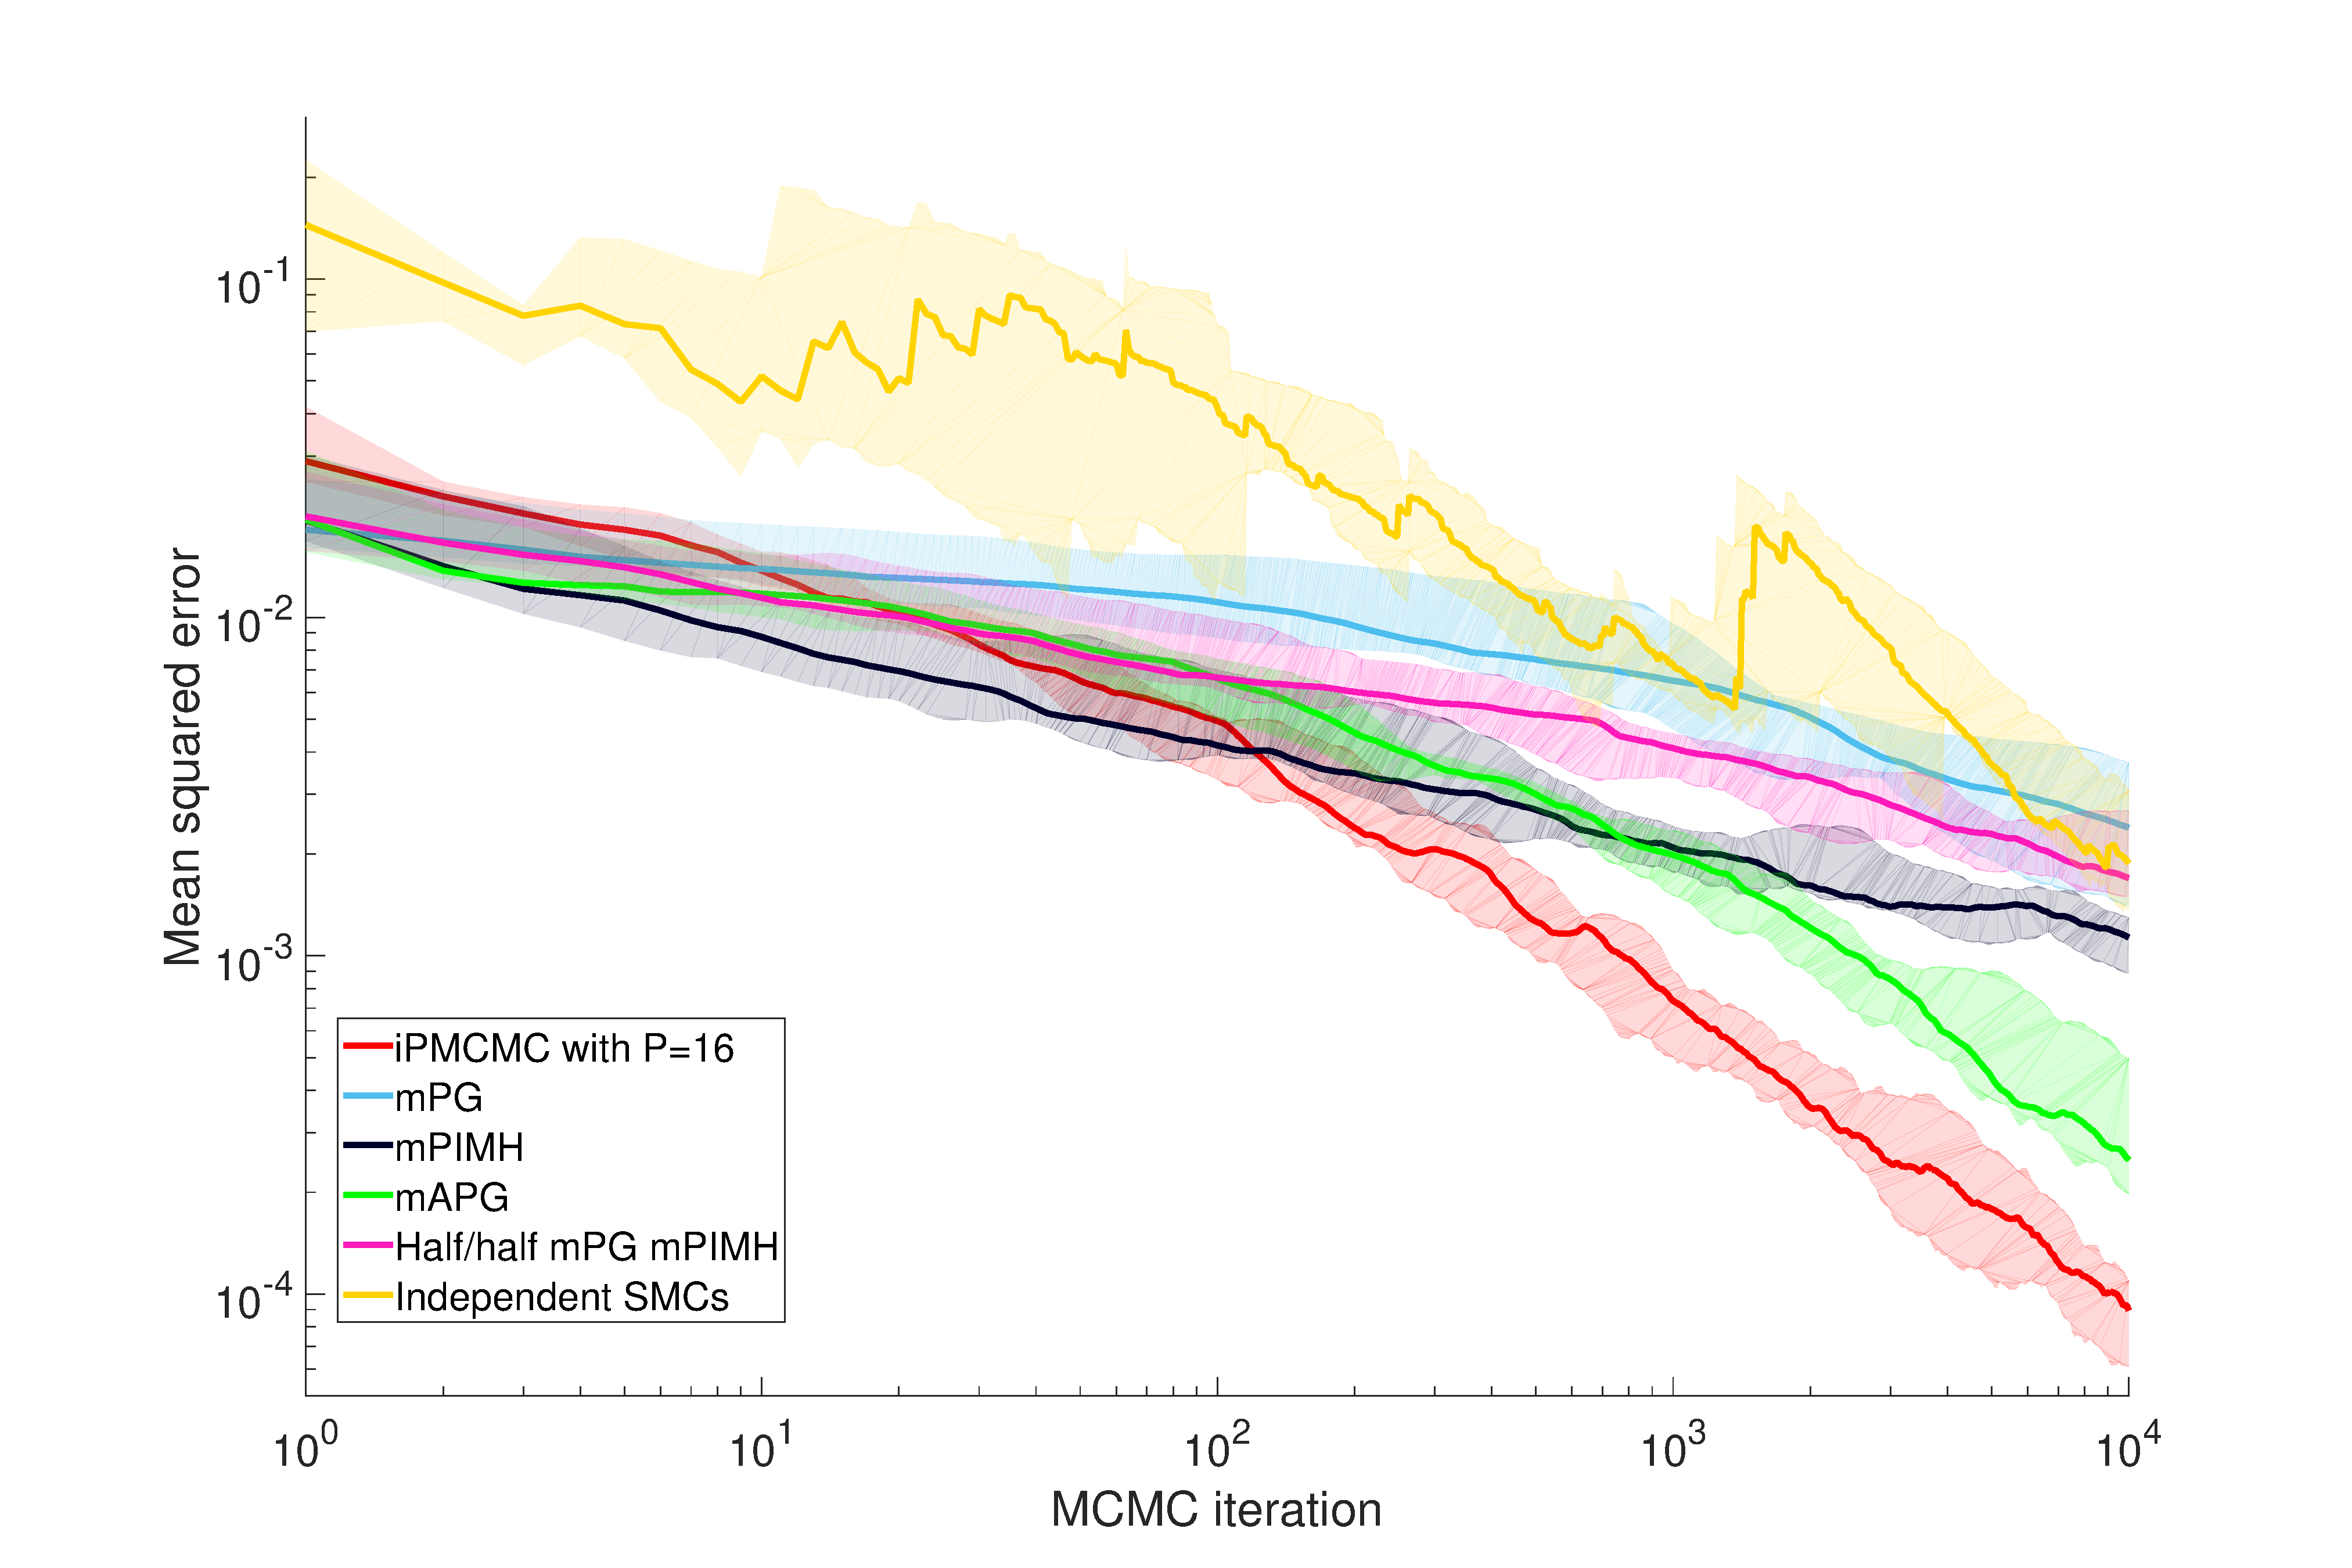
\includegraphics[width=1.1\textwidth,trim={4cm 0 5cm 0},clip]{mean_conv_distributable_lss}}
		\caption{Convergence in mean}
		\label{fig:supp-mean_dist_conv}
	\end{subfigure}
	~ %add desired spacing between images, e. g. ~, \quad, \qquad, \hfill etc. 
	%(or a blank line to force the subfigure onto a new line)
	\begin{subfigure}[t]{0.49\textwidth}
		\makebox[\textwidth][l]{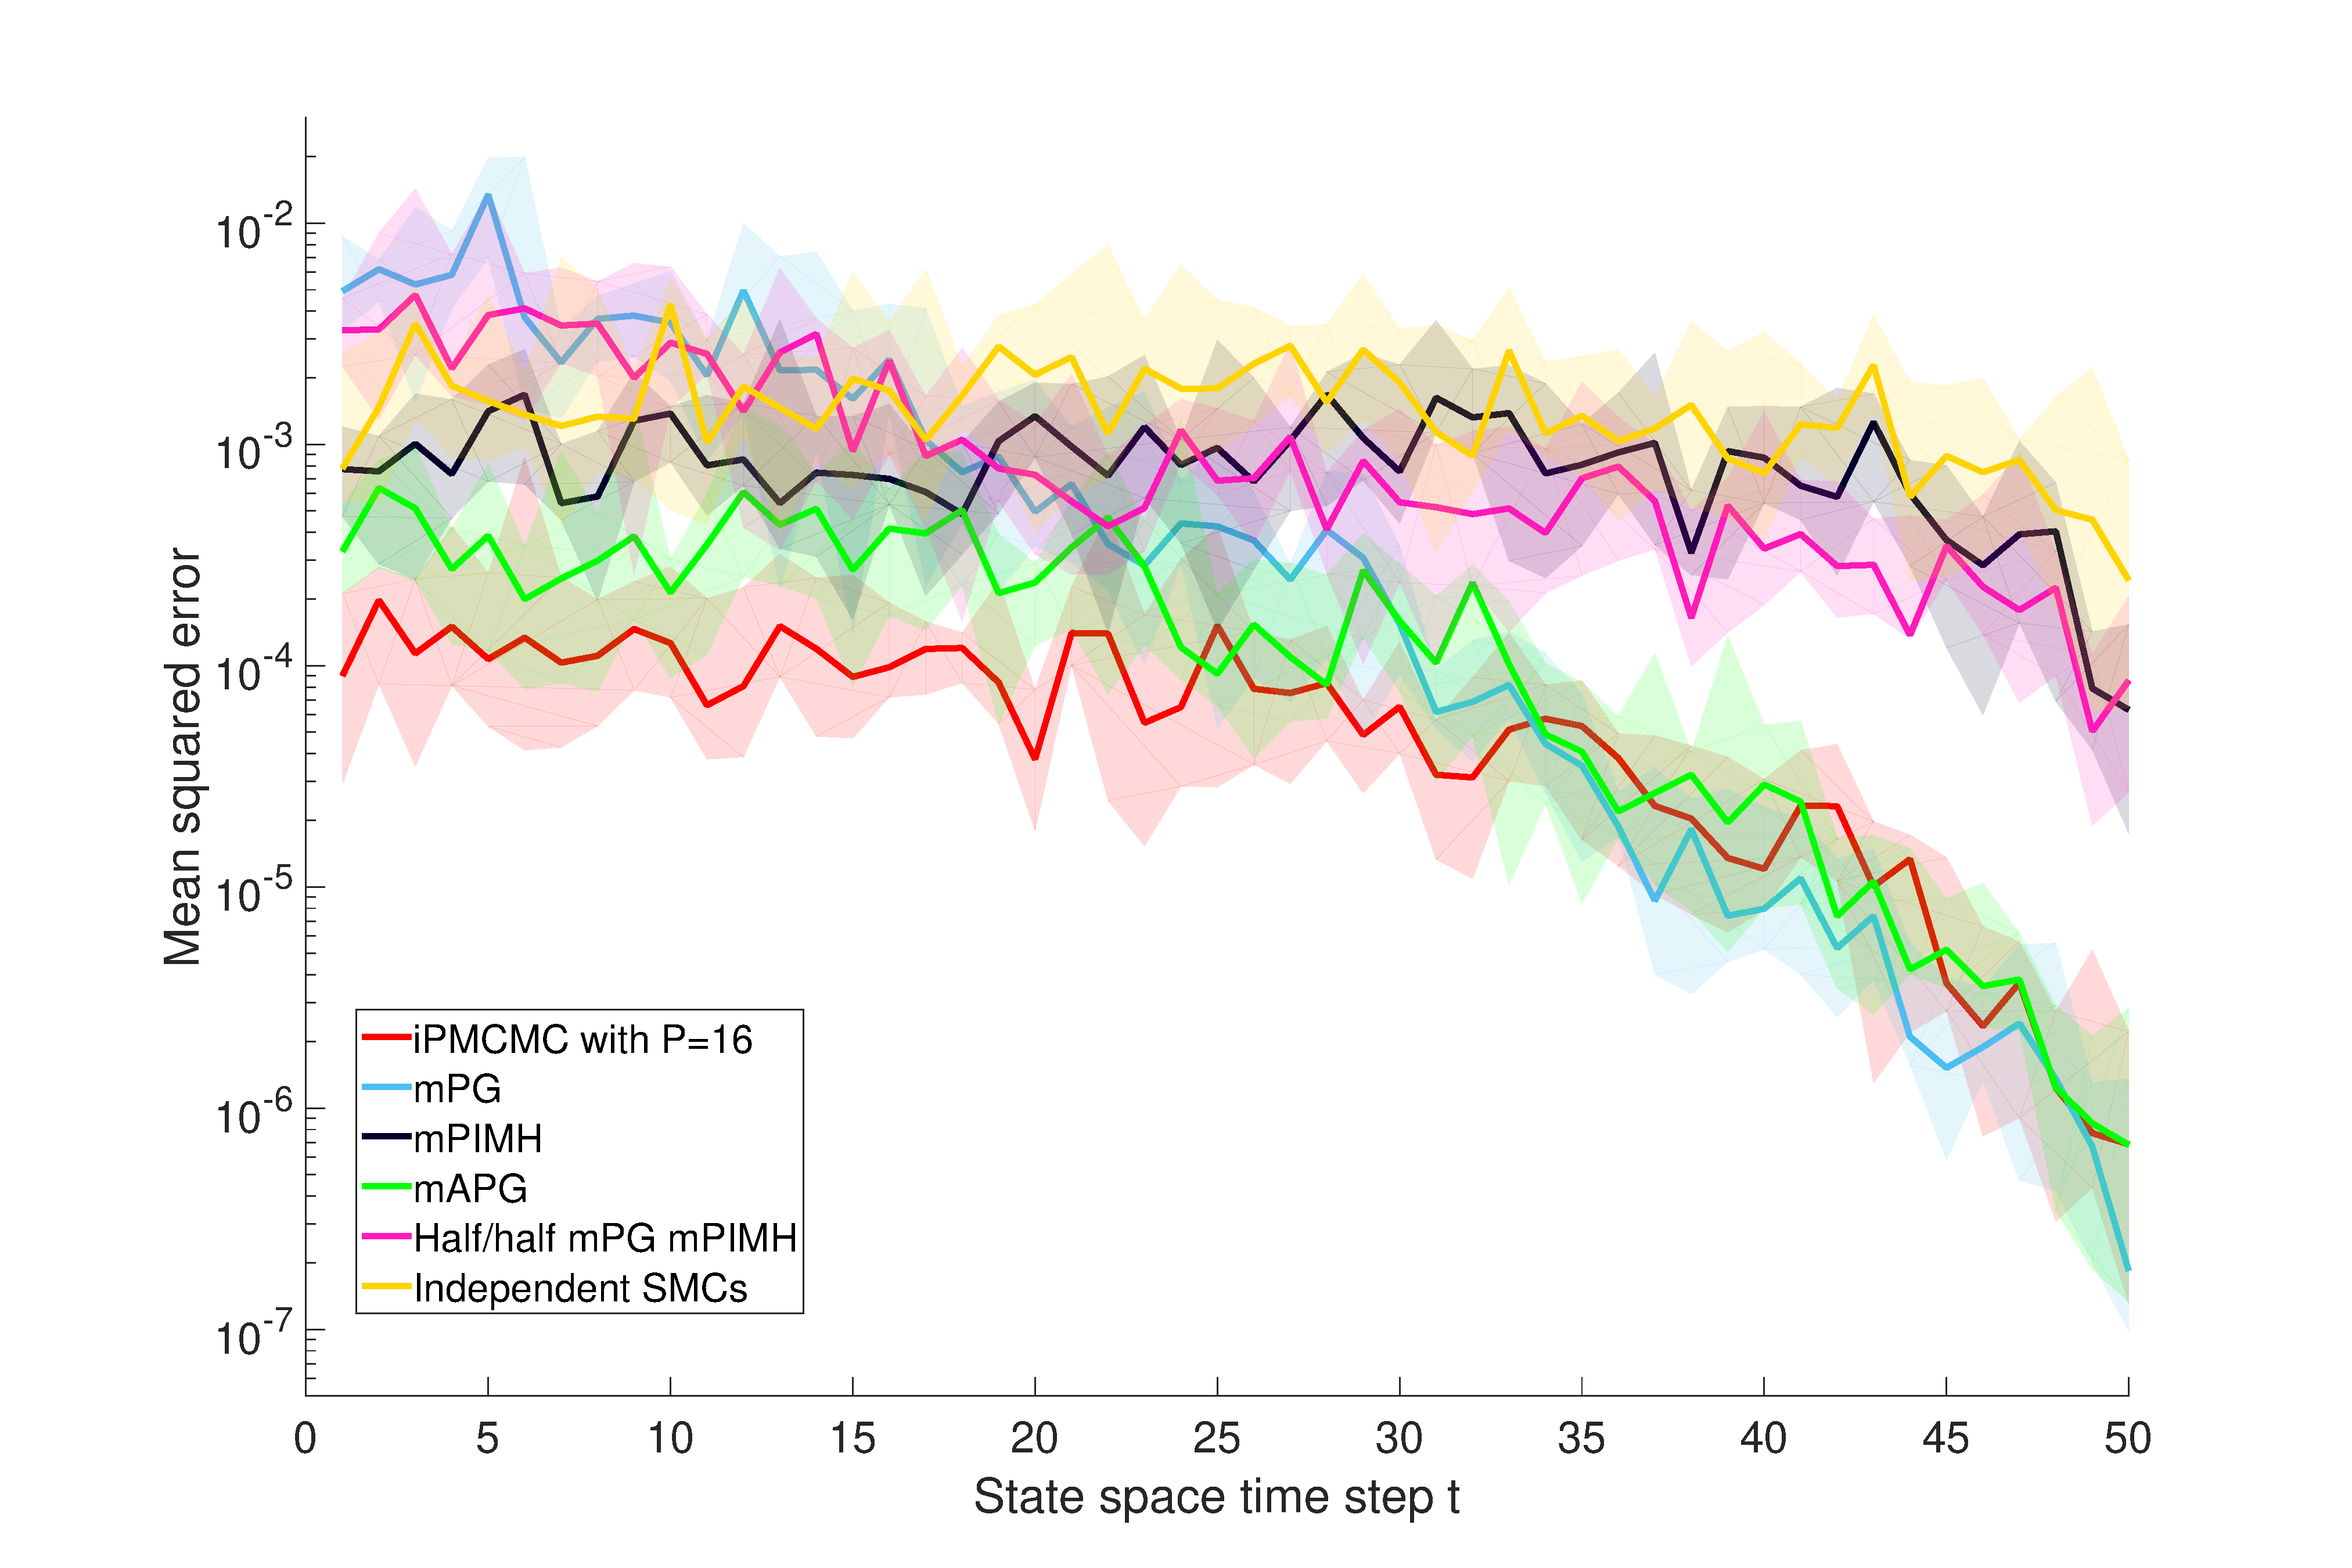
\includegraphics[width=1.1\textwidth,trim={4cm 0 5cm 0},clip]{mean_pos_distributable_lss}}
		\caption{Final error in mean}
		\label{fig:supp-mean_dist_pos}
	\end{subfigure}
	
	\begin{subfigure}[t]{0.49\textwidth}
		\makebox[\textwidth][r]{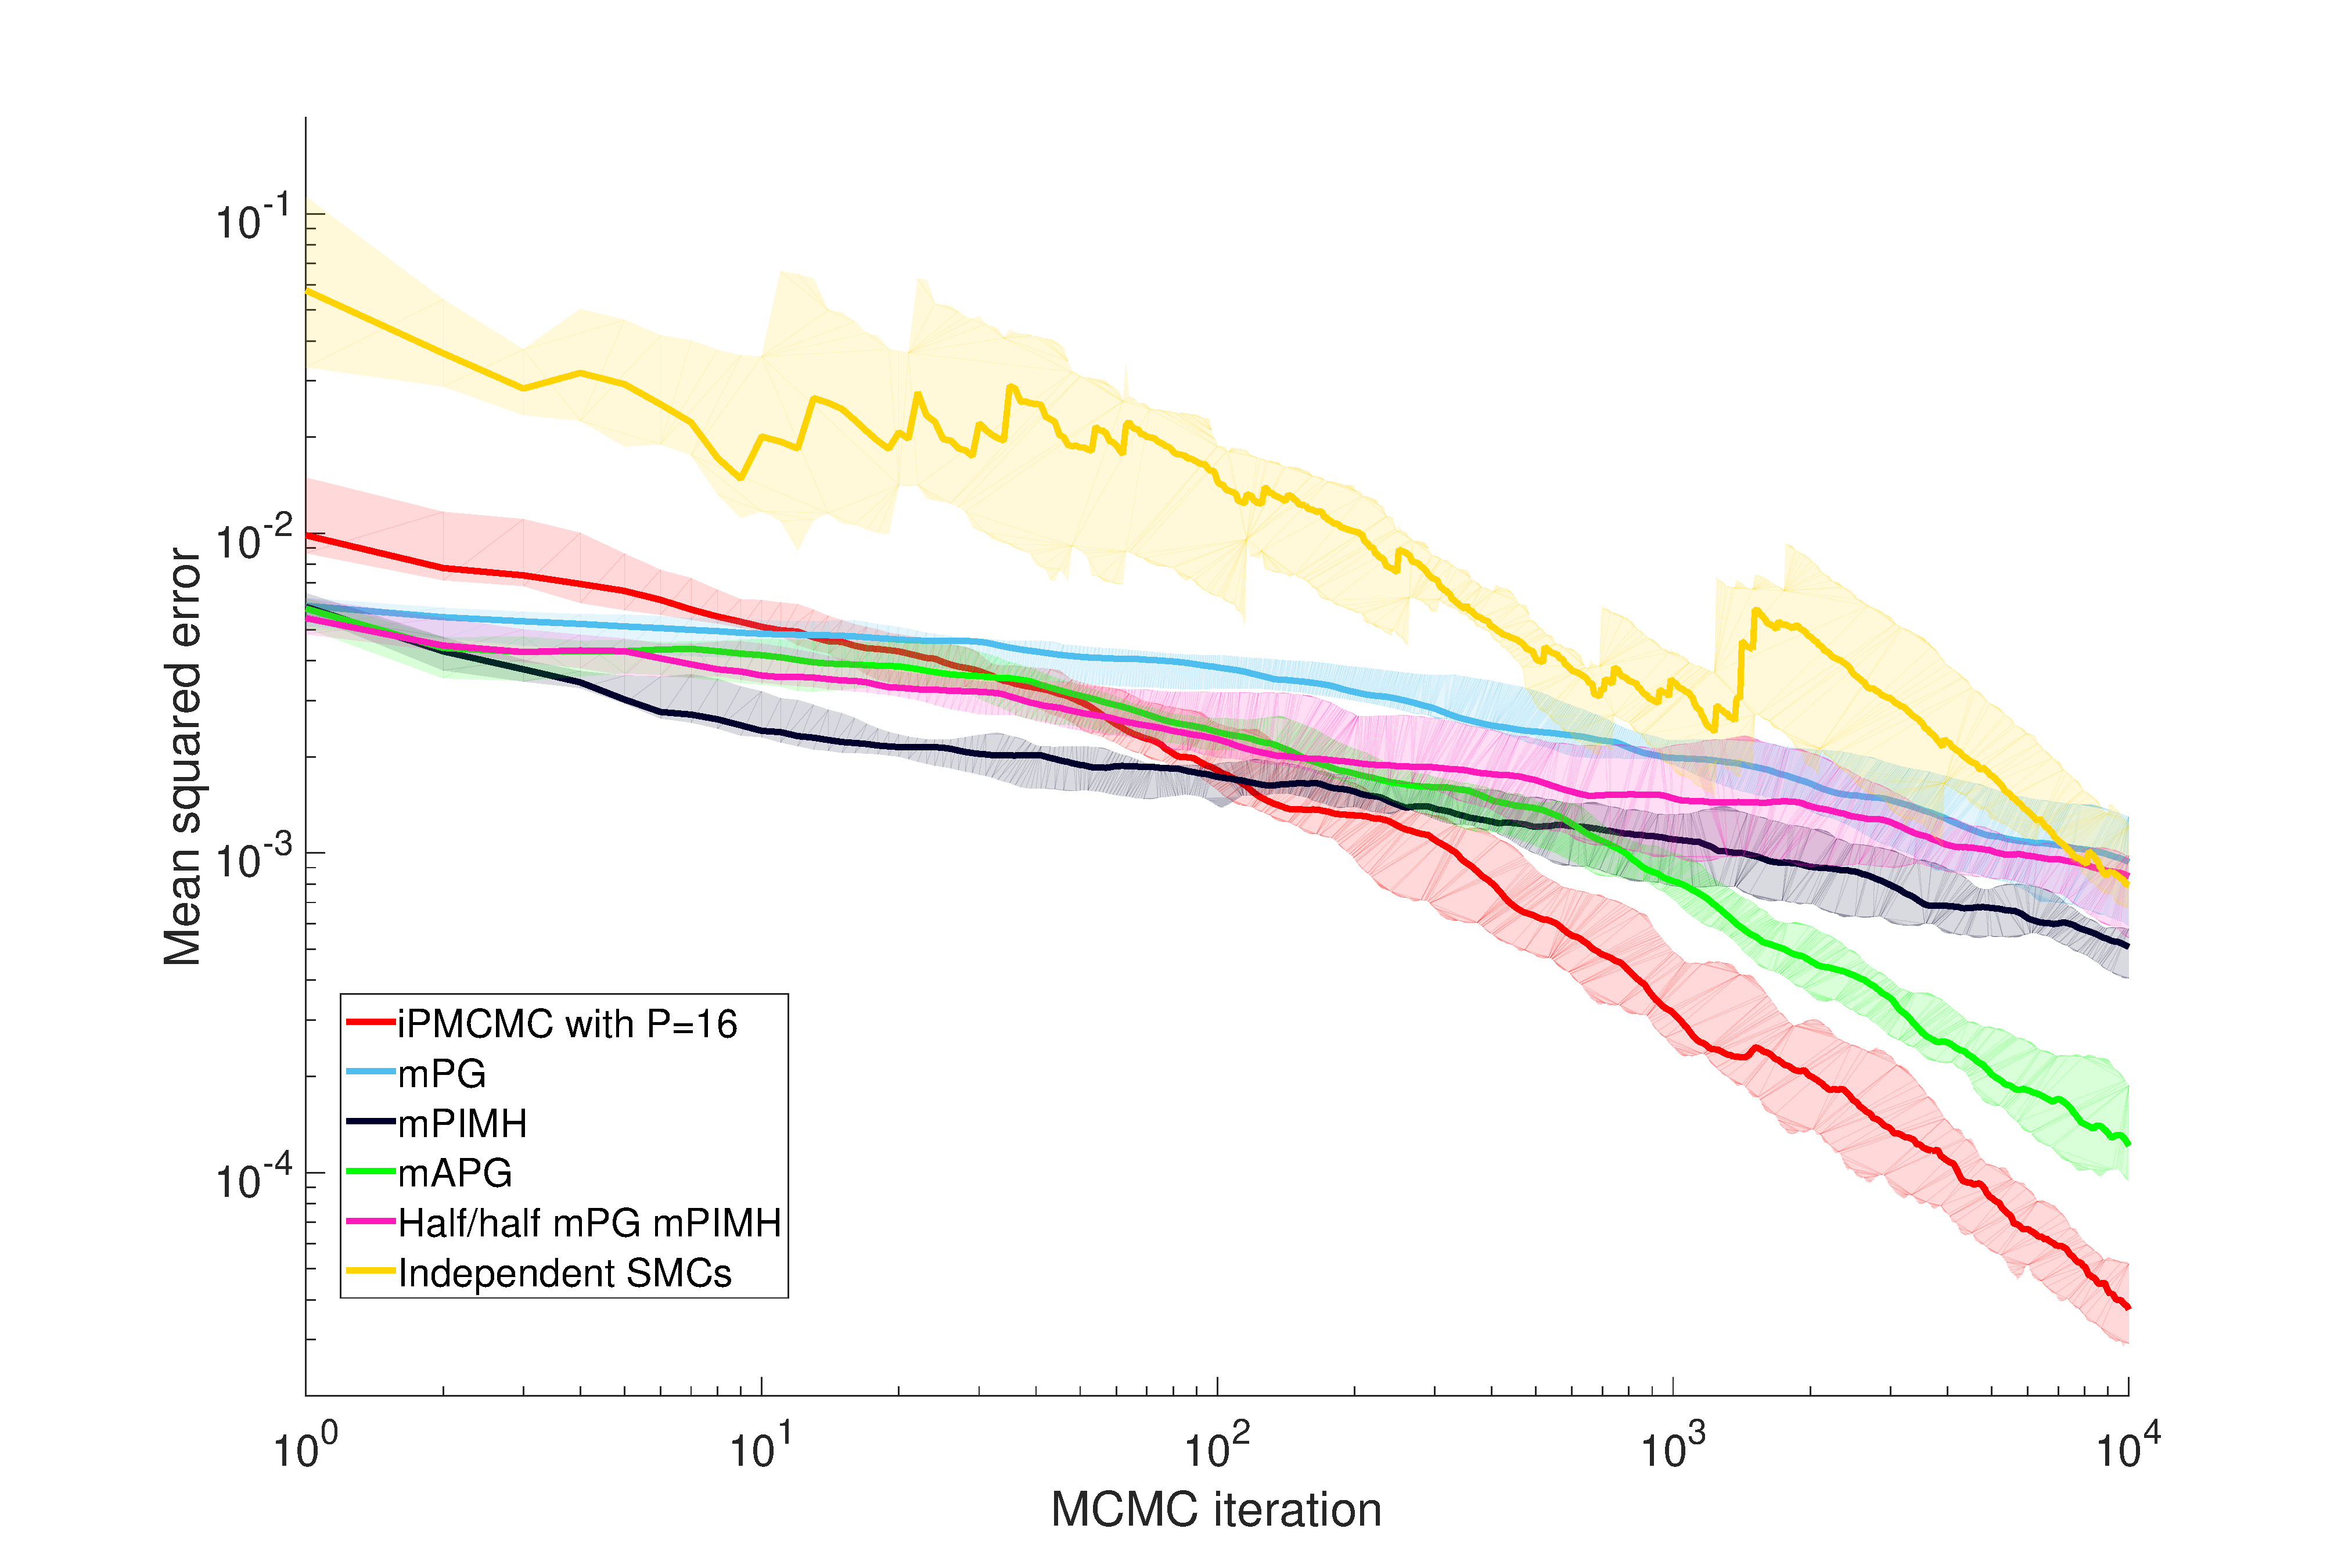
\includegraphics[width=1.1\textwidth,trim={4cm 0 5cm 0},clip]{std_conv_distributable_lss}}
		\caption{Convergence in standard deviation}
		\label{fig:supp-std_dist_conv}
	\end{subfigure}
	~ %add desired spacing between images, e. g. ~, \quad, \qquad, \hfill etc. 
	%(or a blank line to force the subfigure onto a new line)
	\begin{subfigure}[t]{0.49\textwidth}
		\makebox[\textwidth][l]{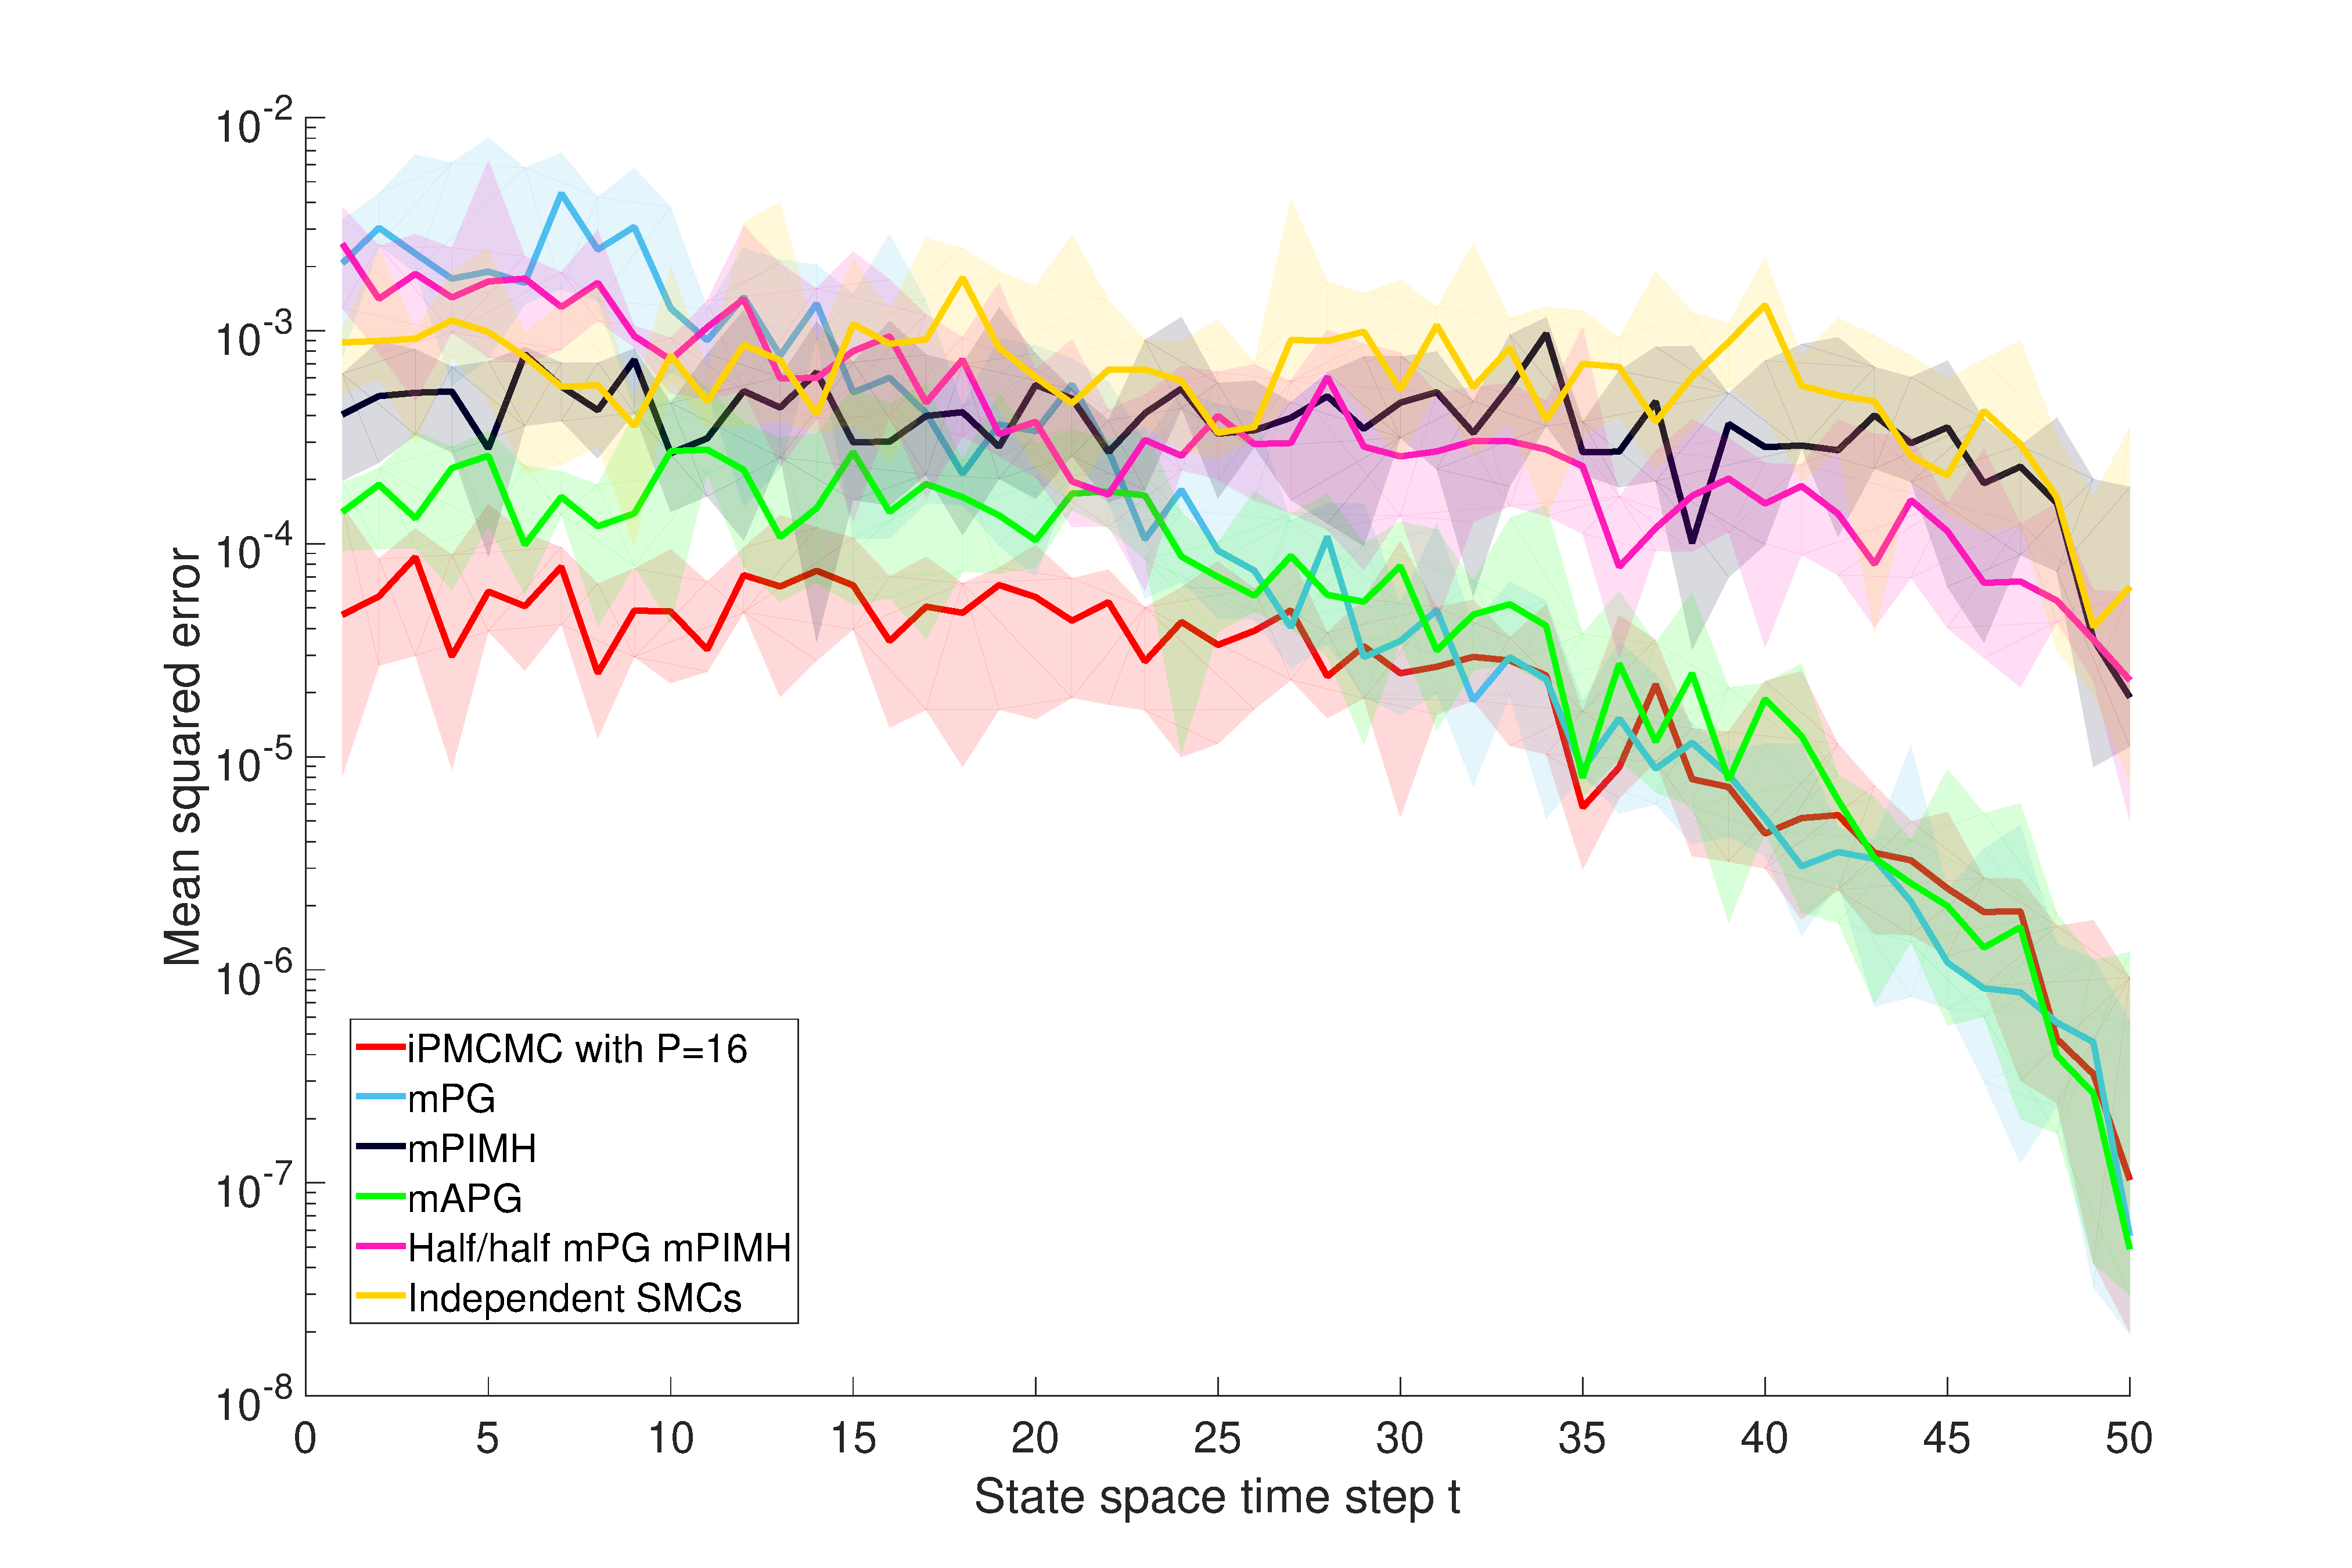
\includegraphics[width=1.1\textwidth,trim={4cm 0 5cm 0},clip]{std_pos_distributable_lss}}
		\caption{Final error in standard deviation}
		\label{fig:supp-std_dist_pos}
	\end{subfigure}	
	\caption{Mean squared error in latent variable mean and standard deviation averaged over all dimensions of the LGSSM as a function of MCMC iteration (left) and position in the state sequence (right) for a selection of paraellelizable SMC and PMCMC methods.  See figure 3 in main paper for more details. \label{fig:supp-distributable_error_lss}}
\end{figure*}

\begin{figure*}[p]
	\centering
\begin{subfigure}[t]{0.49\textwidth}
	\makebox[\textwidth][r]{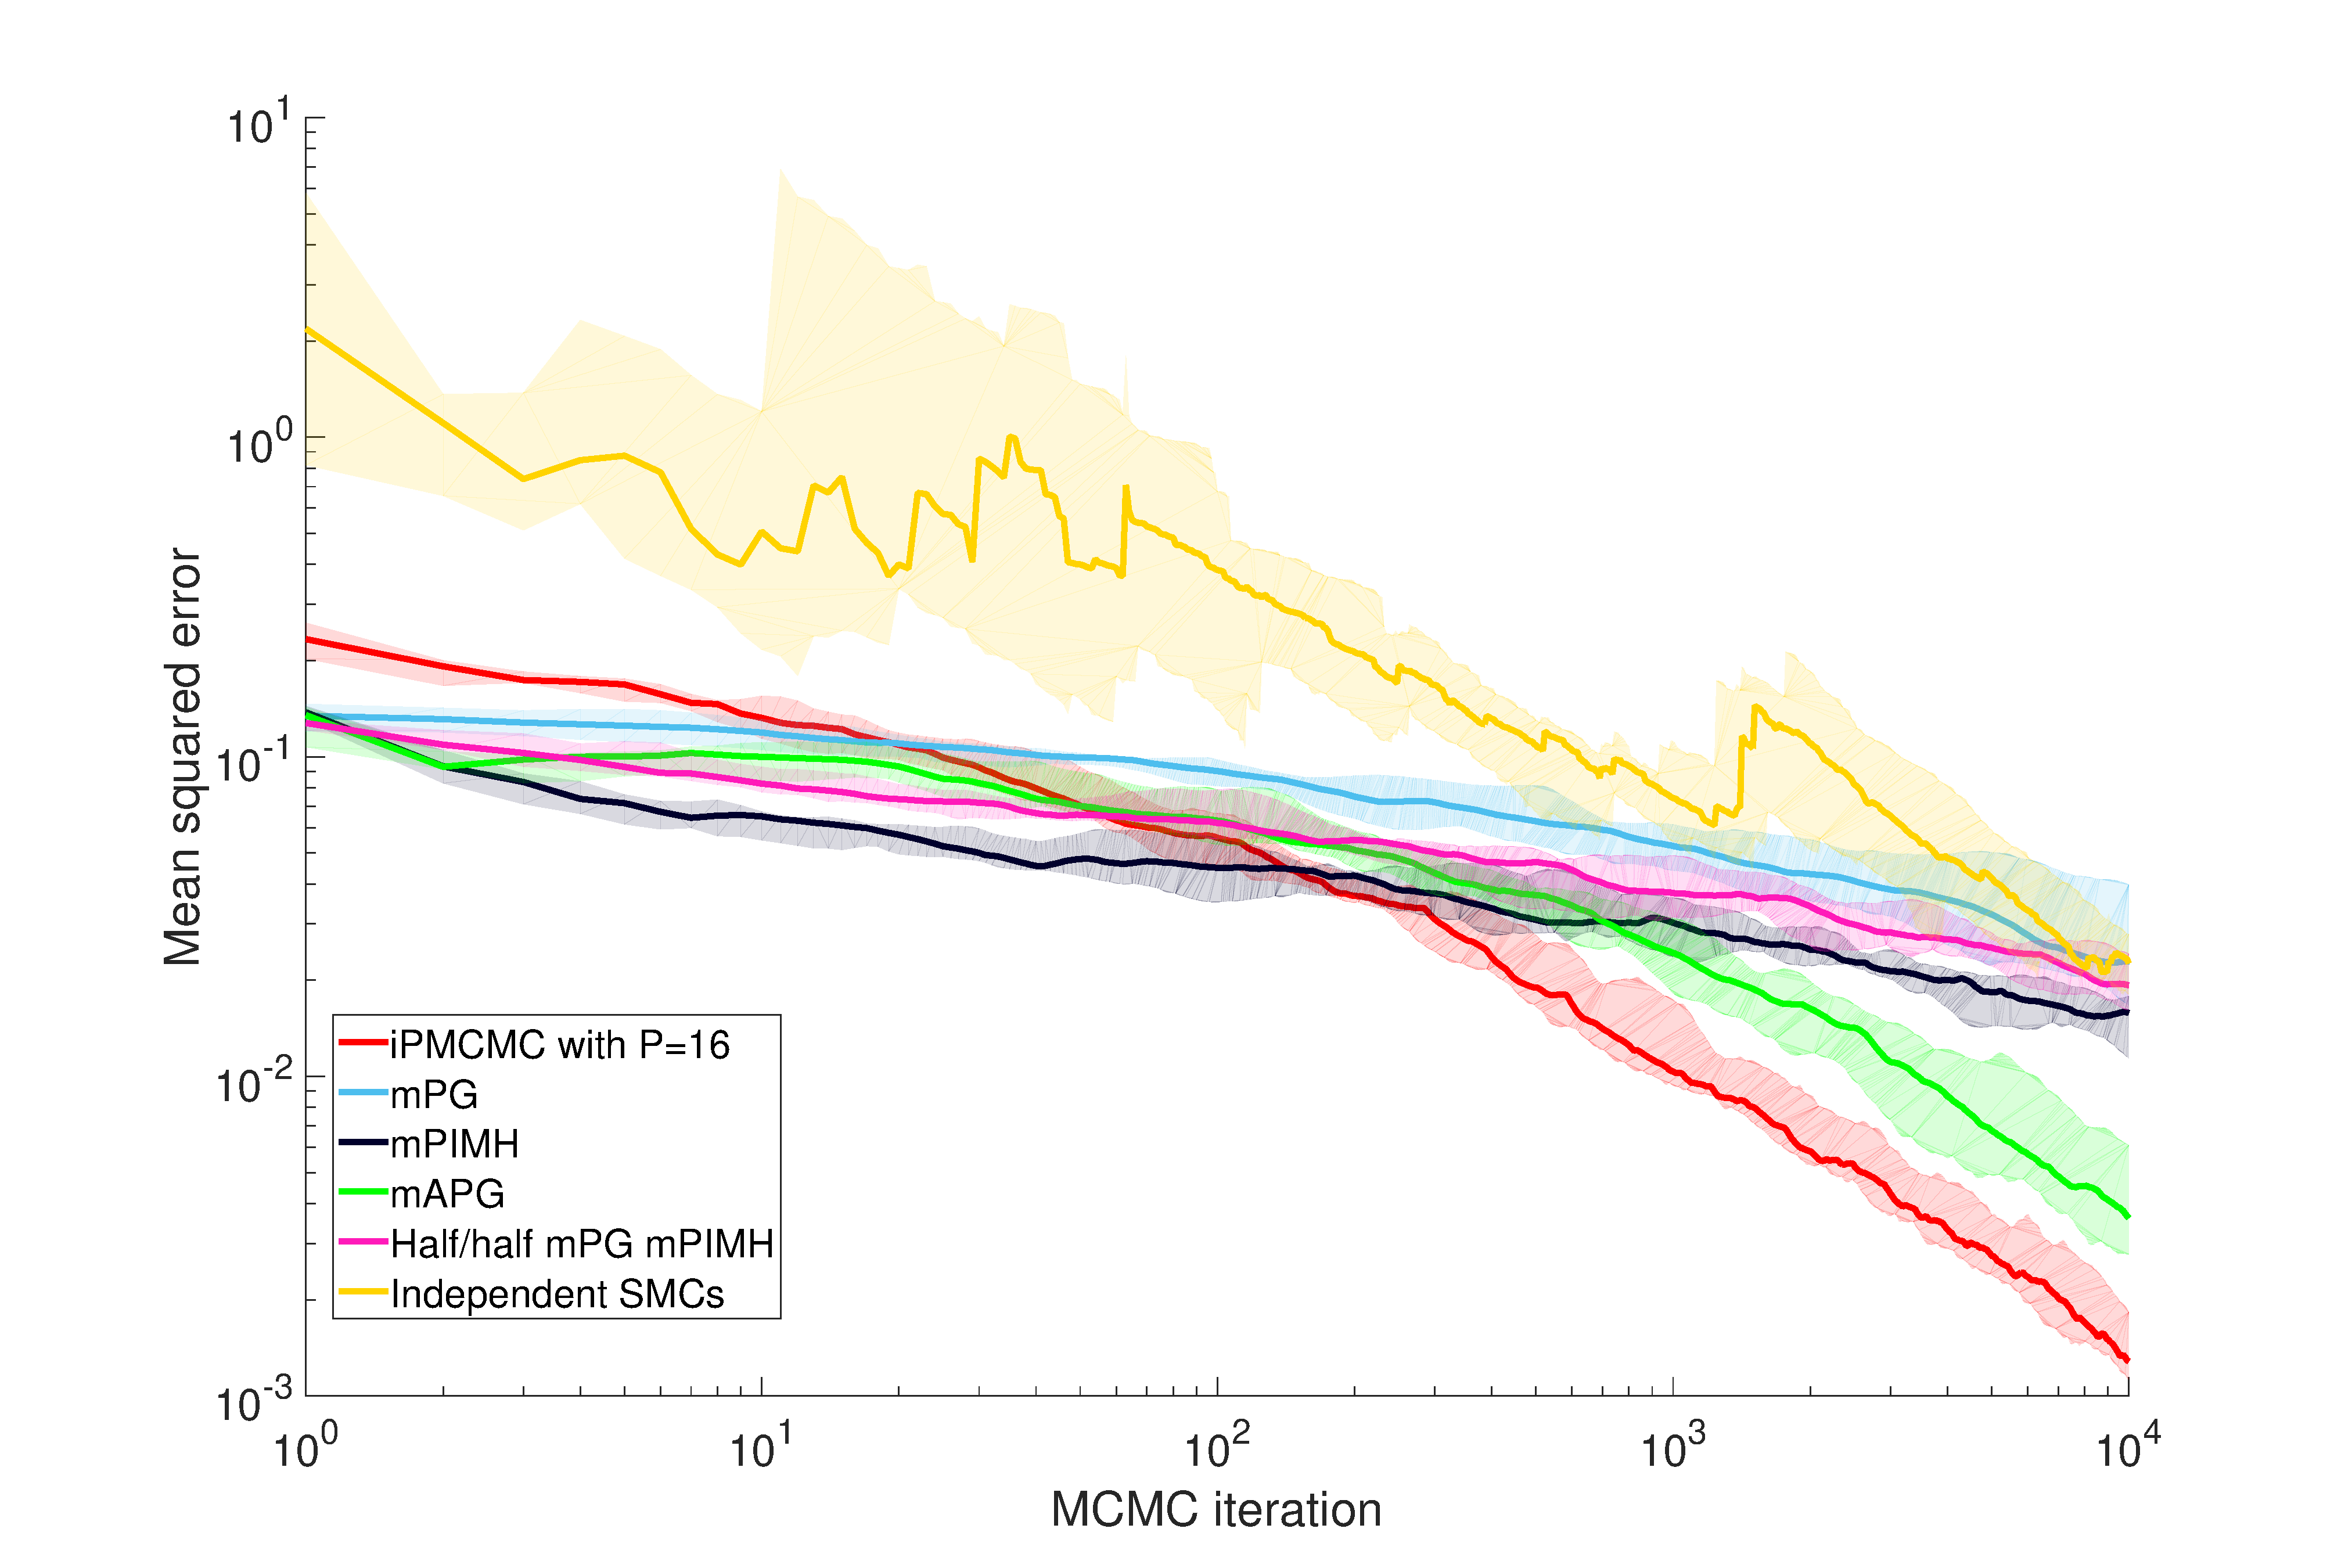
\includegraphics[width=1.1\textwidth,trim={4cm 0 5cm 0},clip]{skewness_conv_distributable_lss}}
	\caption{Convergence in skewness}
	\label{fig:supp-ske_dist_conv}
\end{subfigure}
~ %add desired spacing between images, e. g. ~, \quad, \qquad, \hfill etc. 
%(or a blank line to force the subfigure onto a new line)
\begin{subfigure}[t]{0.49\textwidth}
	\makebox[\textwidth][l]{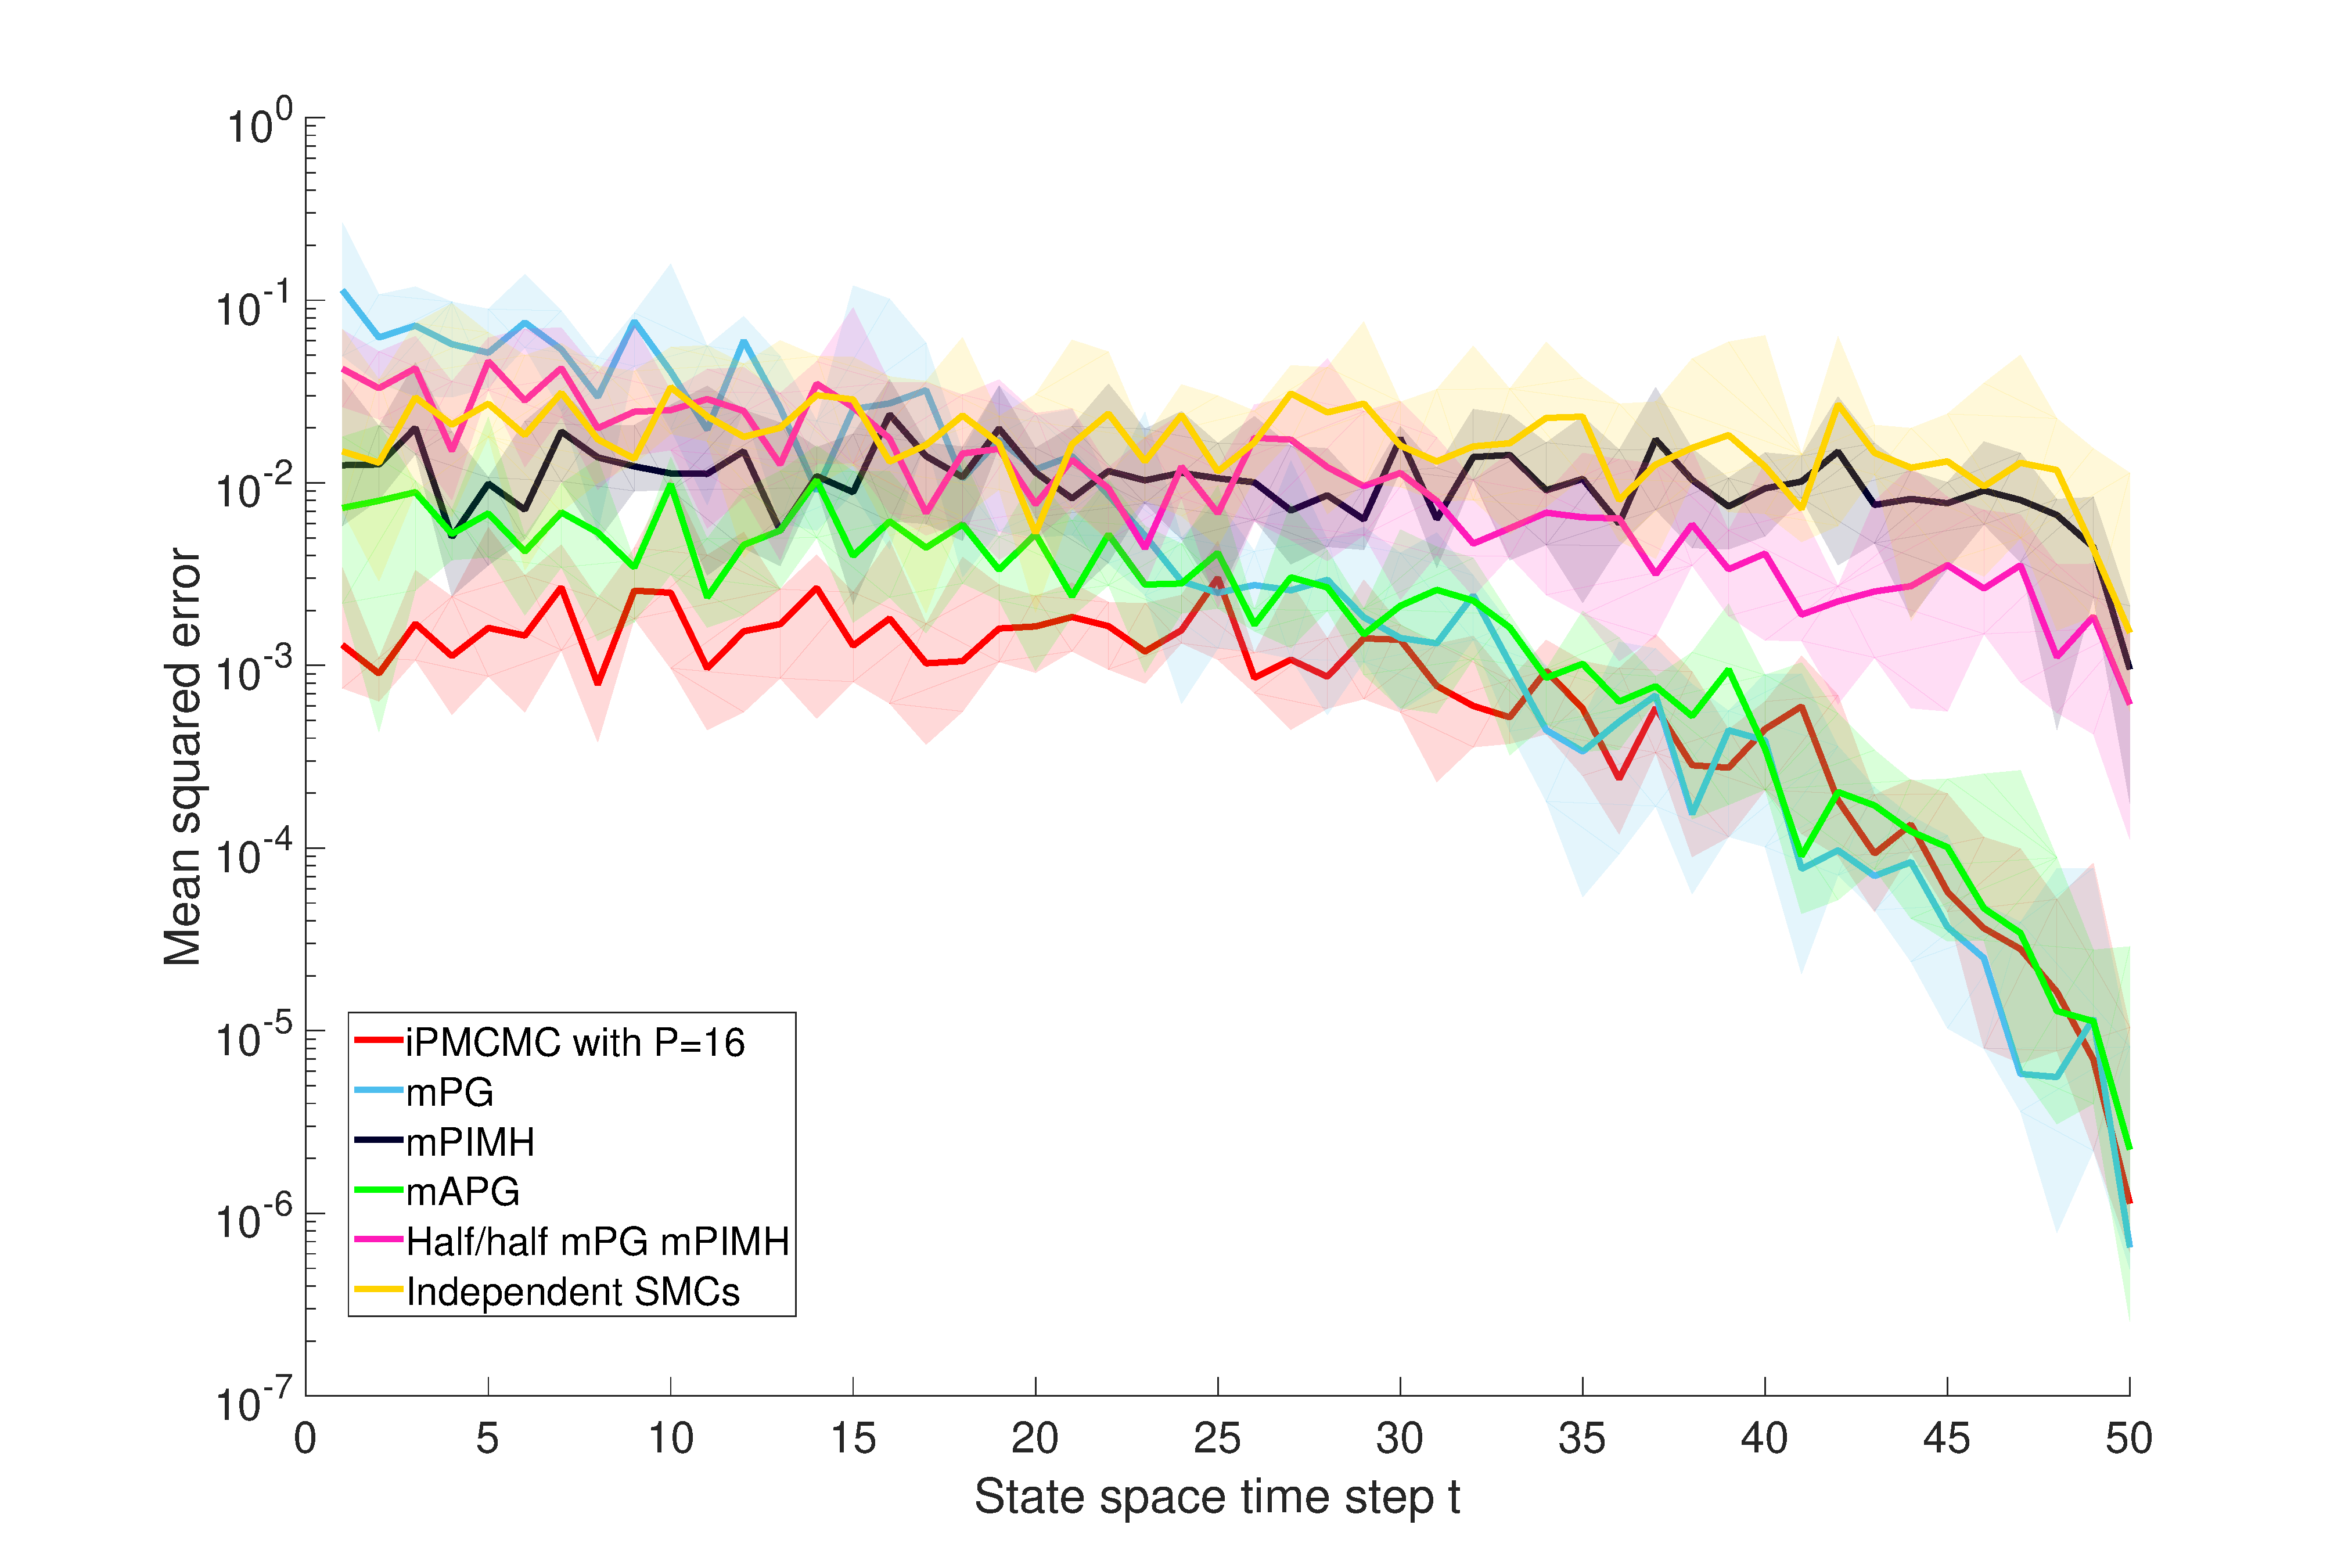
\includegraphics[width=1.1\textwidth,trim={4cm 0 5cm 0},clip]{skewness_pos_distributable_lss}}
	\caption{Final error in skewness}
	\label{fig:supp-ske_dist_pos}
\end{subfigure}	

\begin{subfigure}[t]{0.49\textwidth}
	\makebox[\textwidth][r]{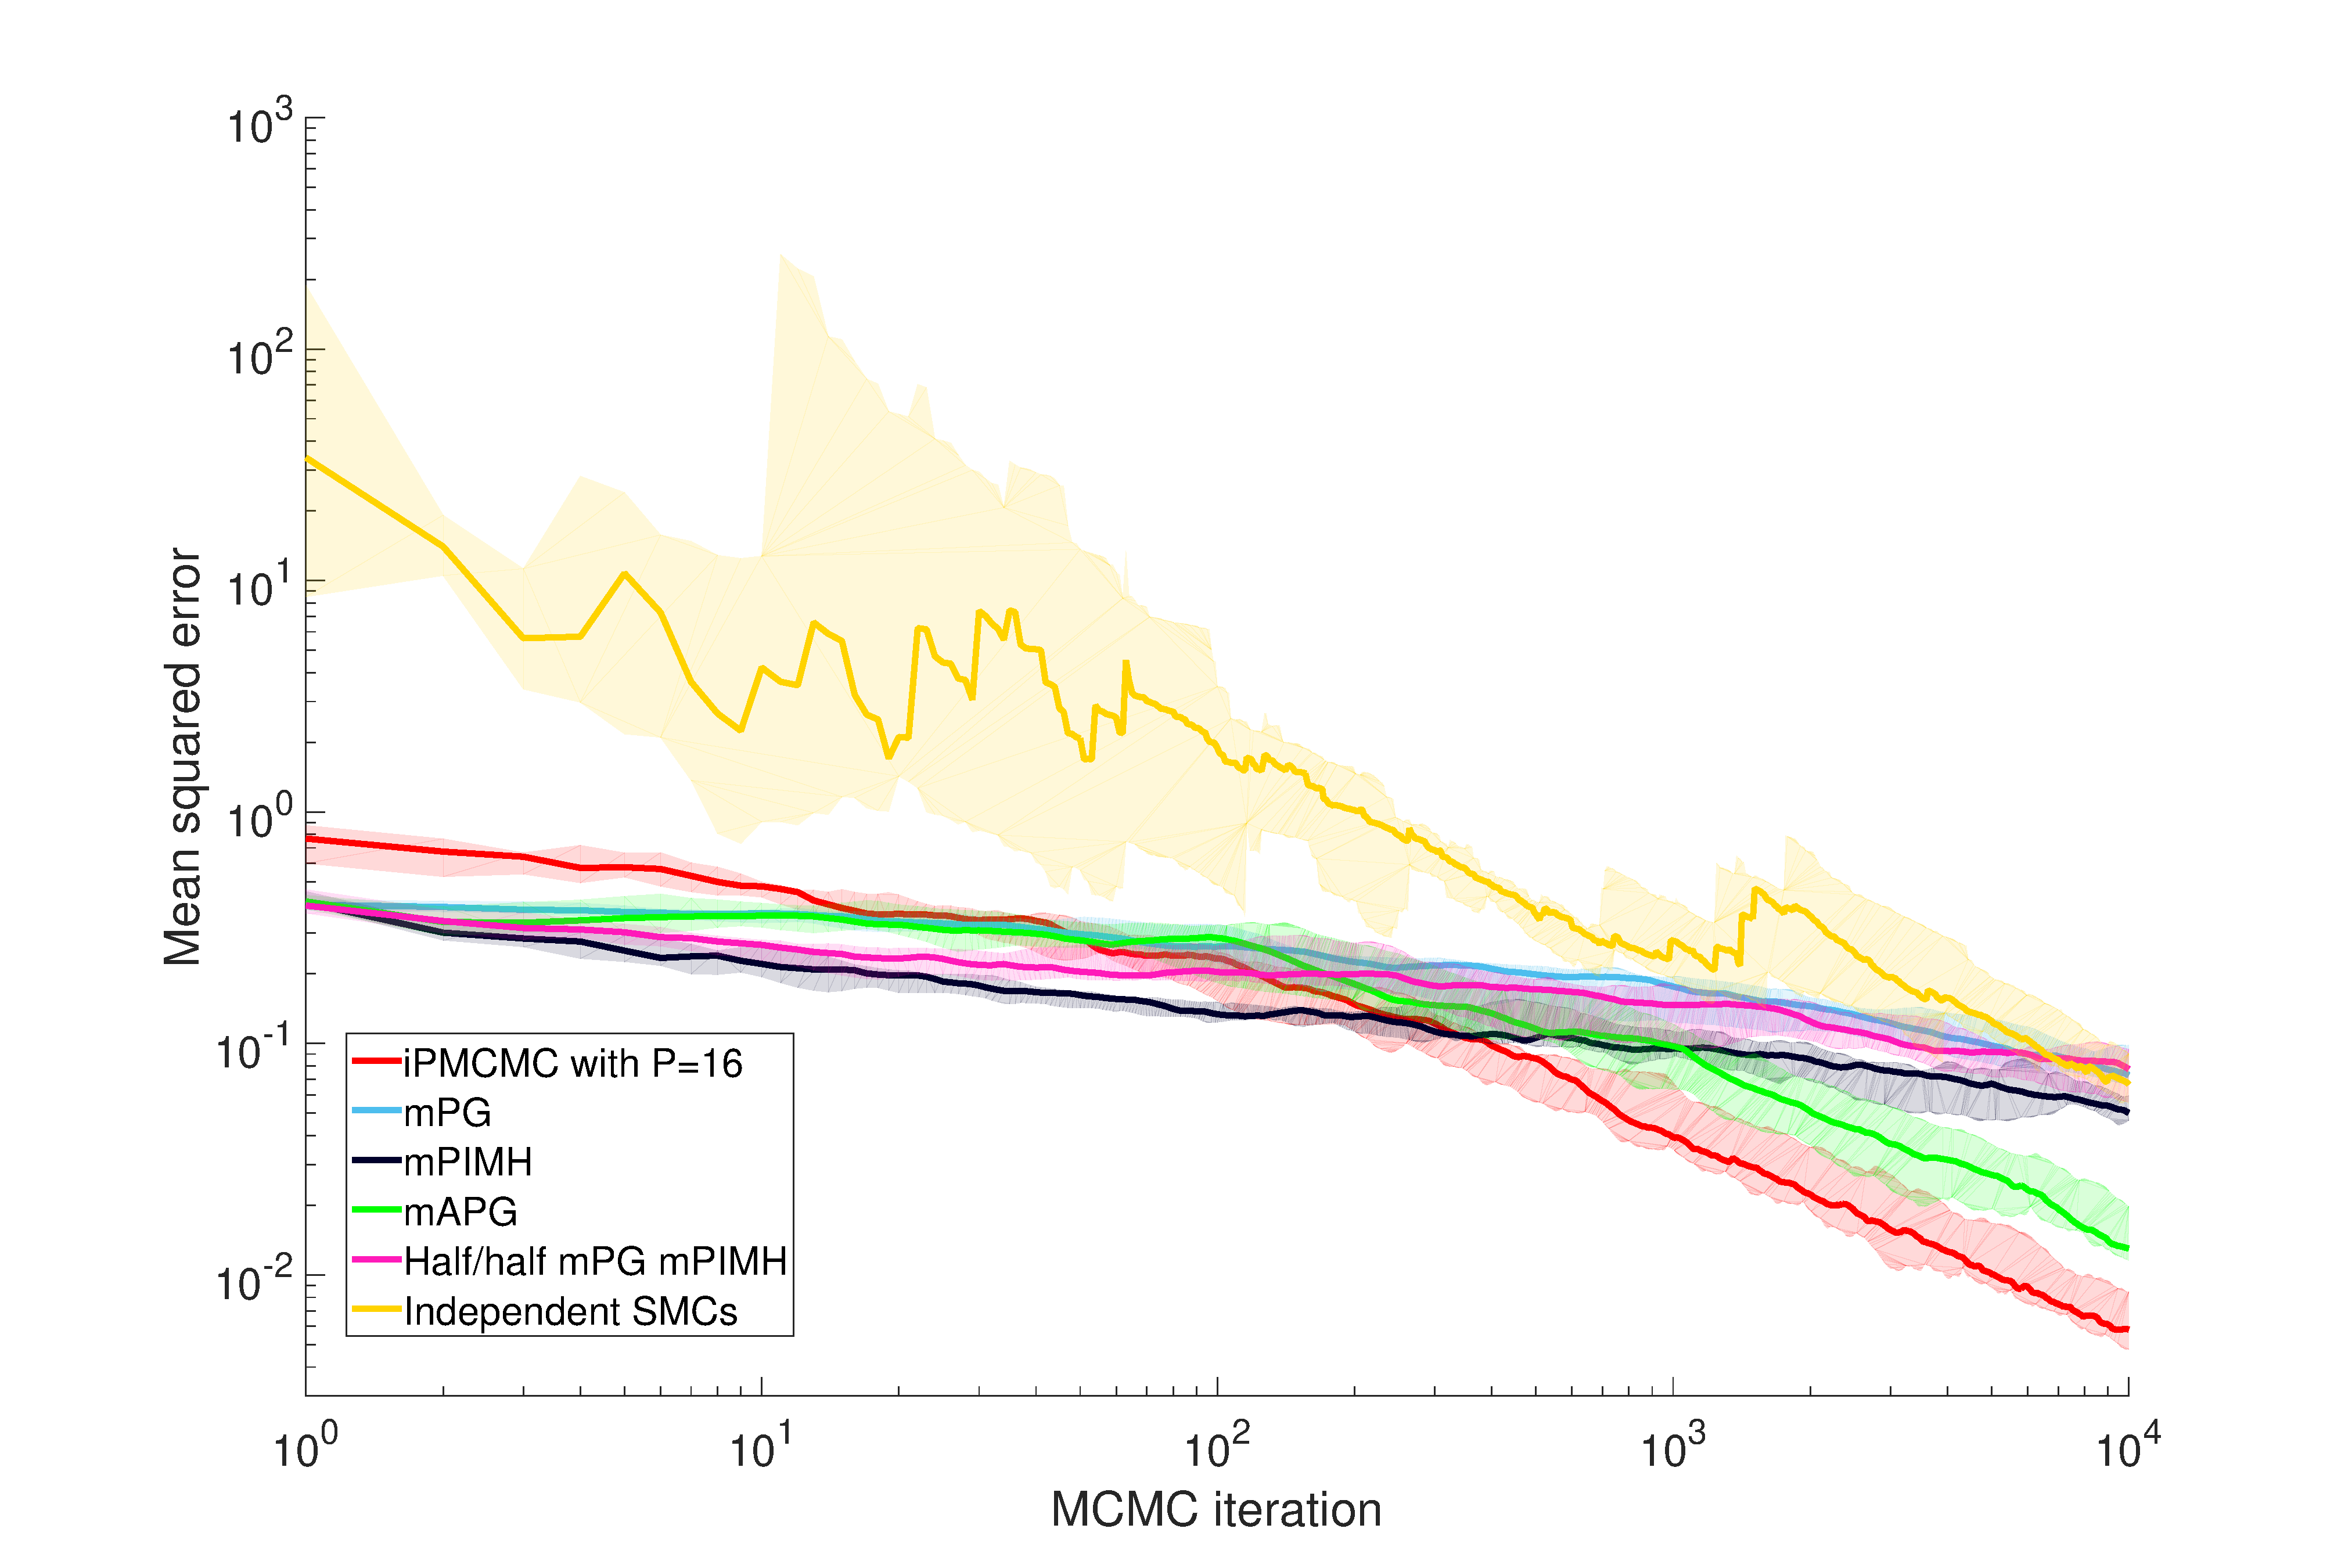
\includegraphics[width=1.1\textwidth,trim={4cm 0 5cm 0},clip]{kurtosis_conv_distributable_lss}}
	\caption{Convergence in kurtosis}
	\label{fig:supp-kurt_dist_conv}
\end{subfigure}
~ %add desired spacing between images, e. g. ~, \quad, \qquad, \hfill etc. 
%(or a blank line to force the subfigure onto a new line)
\begin{subfigure}[t]{0.49\textwidth}
	\makebox[\textwidth][l]{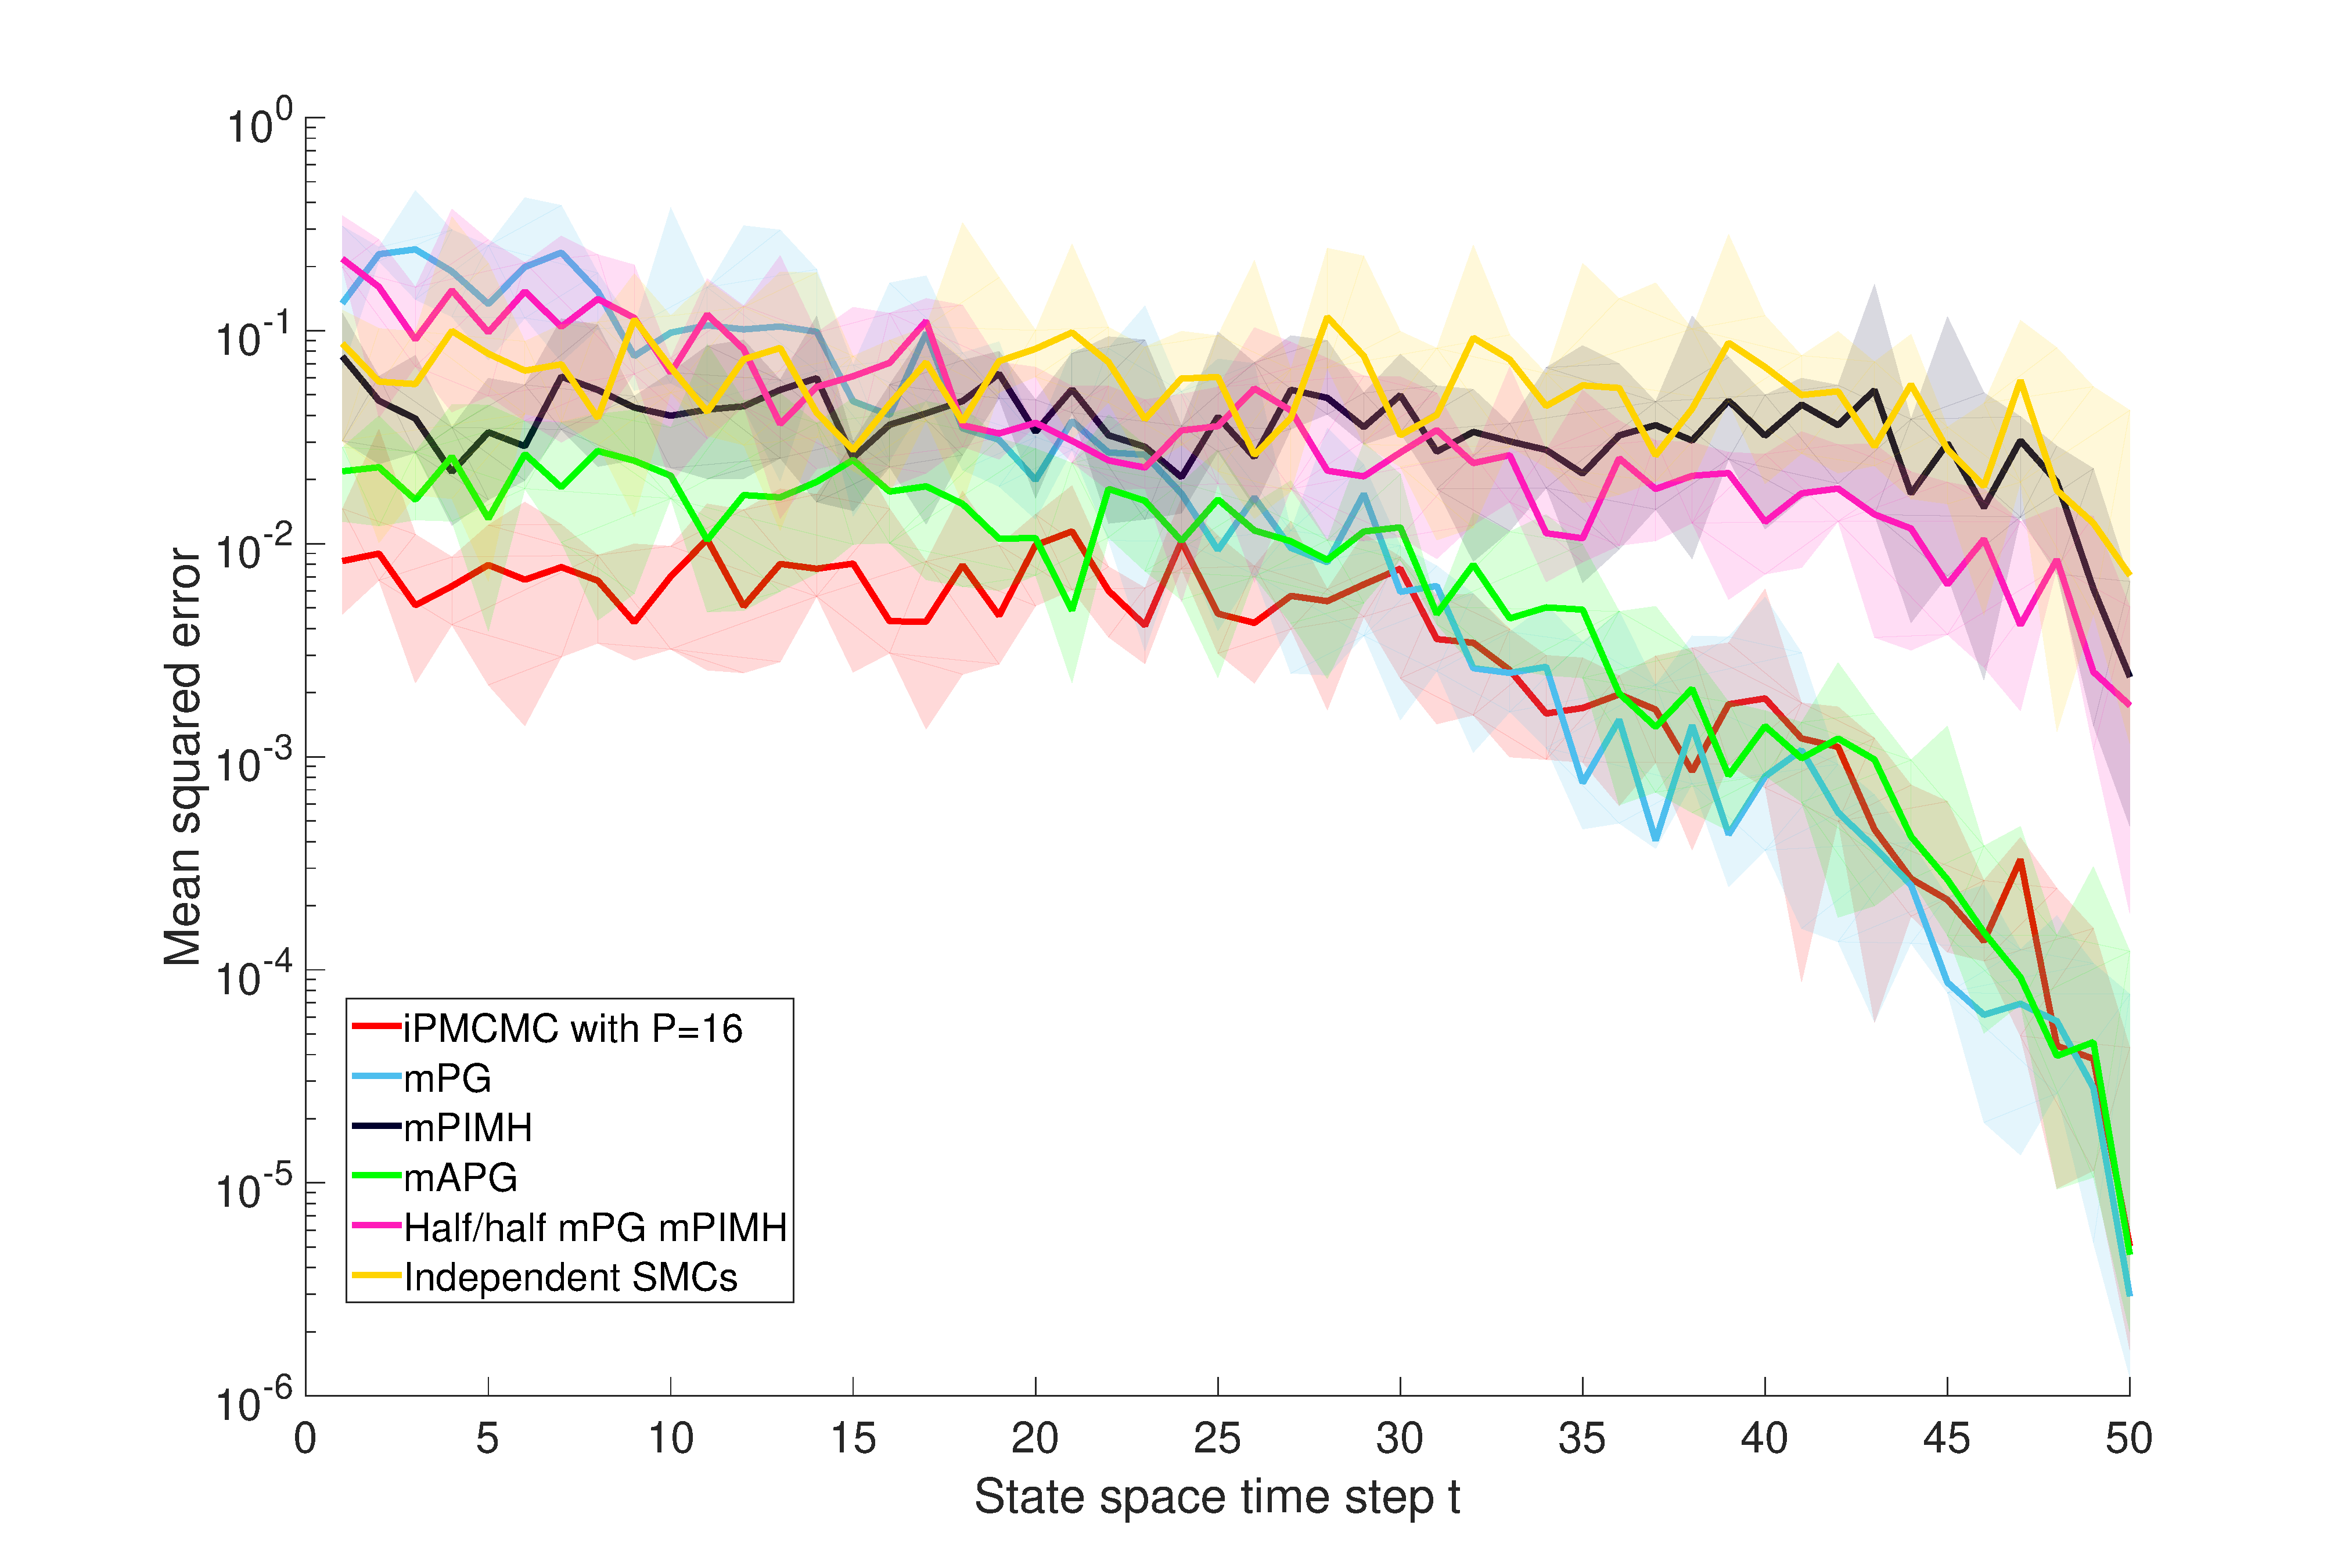
\includegraphics[width=1.1\textwidth,trim={4cm 0 5cm 0},clip]{kurtosis_pos_distributable_lss}}
	\caption{Final error in kurtosis}
	\label{fig:supp-kurt_dist_pos}
\end{subfigure}	
	\caption{Mean squared error in latent variable skewness and kurtosis averaged over all dimensions of the LGSSM as a function of MCMC iteration (left) and position in the state sequence (right) for a selection of paraellelizable SMC and PMCMC methods.  See figure 3 in main paper for more details. \label{fig:supp-distributable_error_lss2}}
\end{figure*}


\begin{figure*}[p]
	\centering
	\begin{subfigure}[t]{0.49\textwidth}
		\makebox[\textwidth][r]{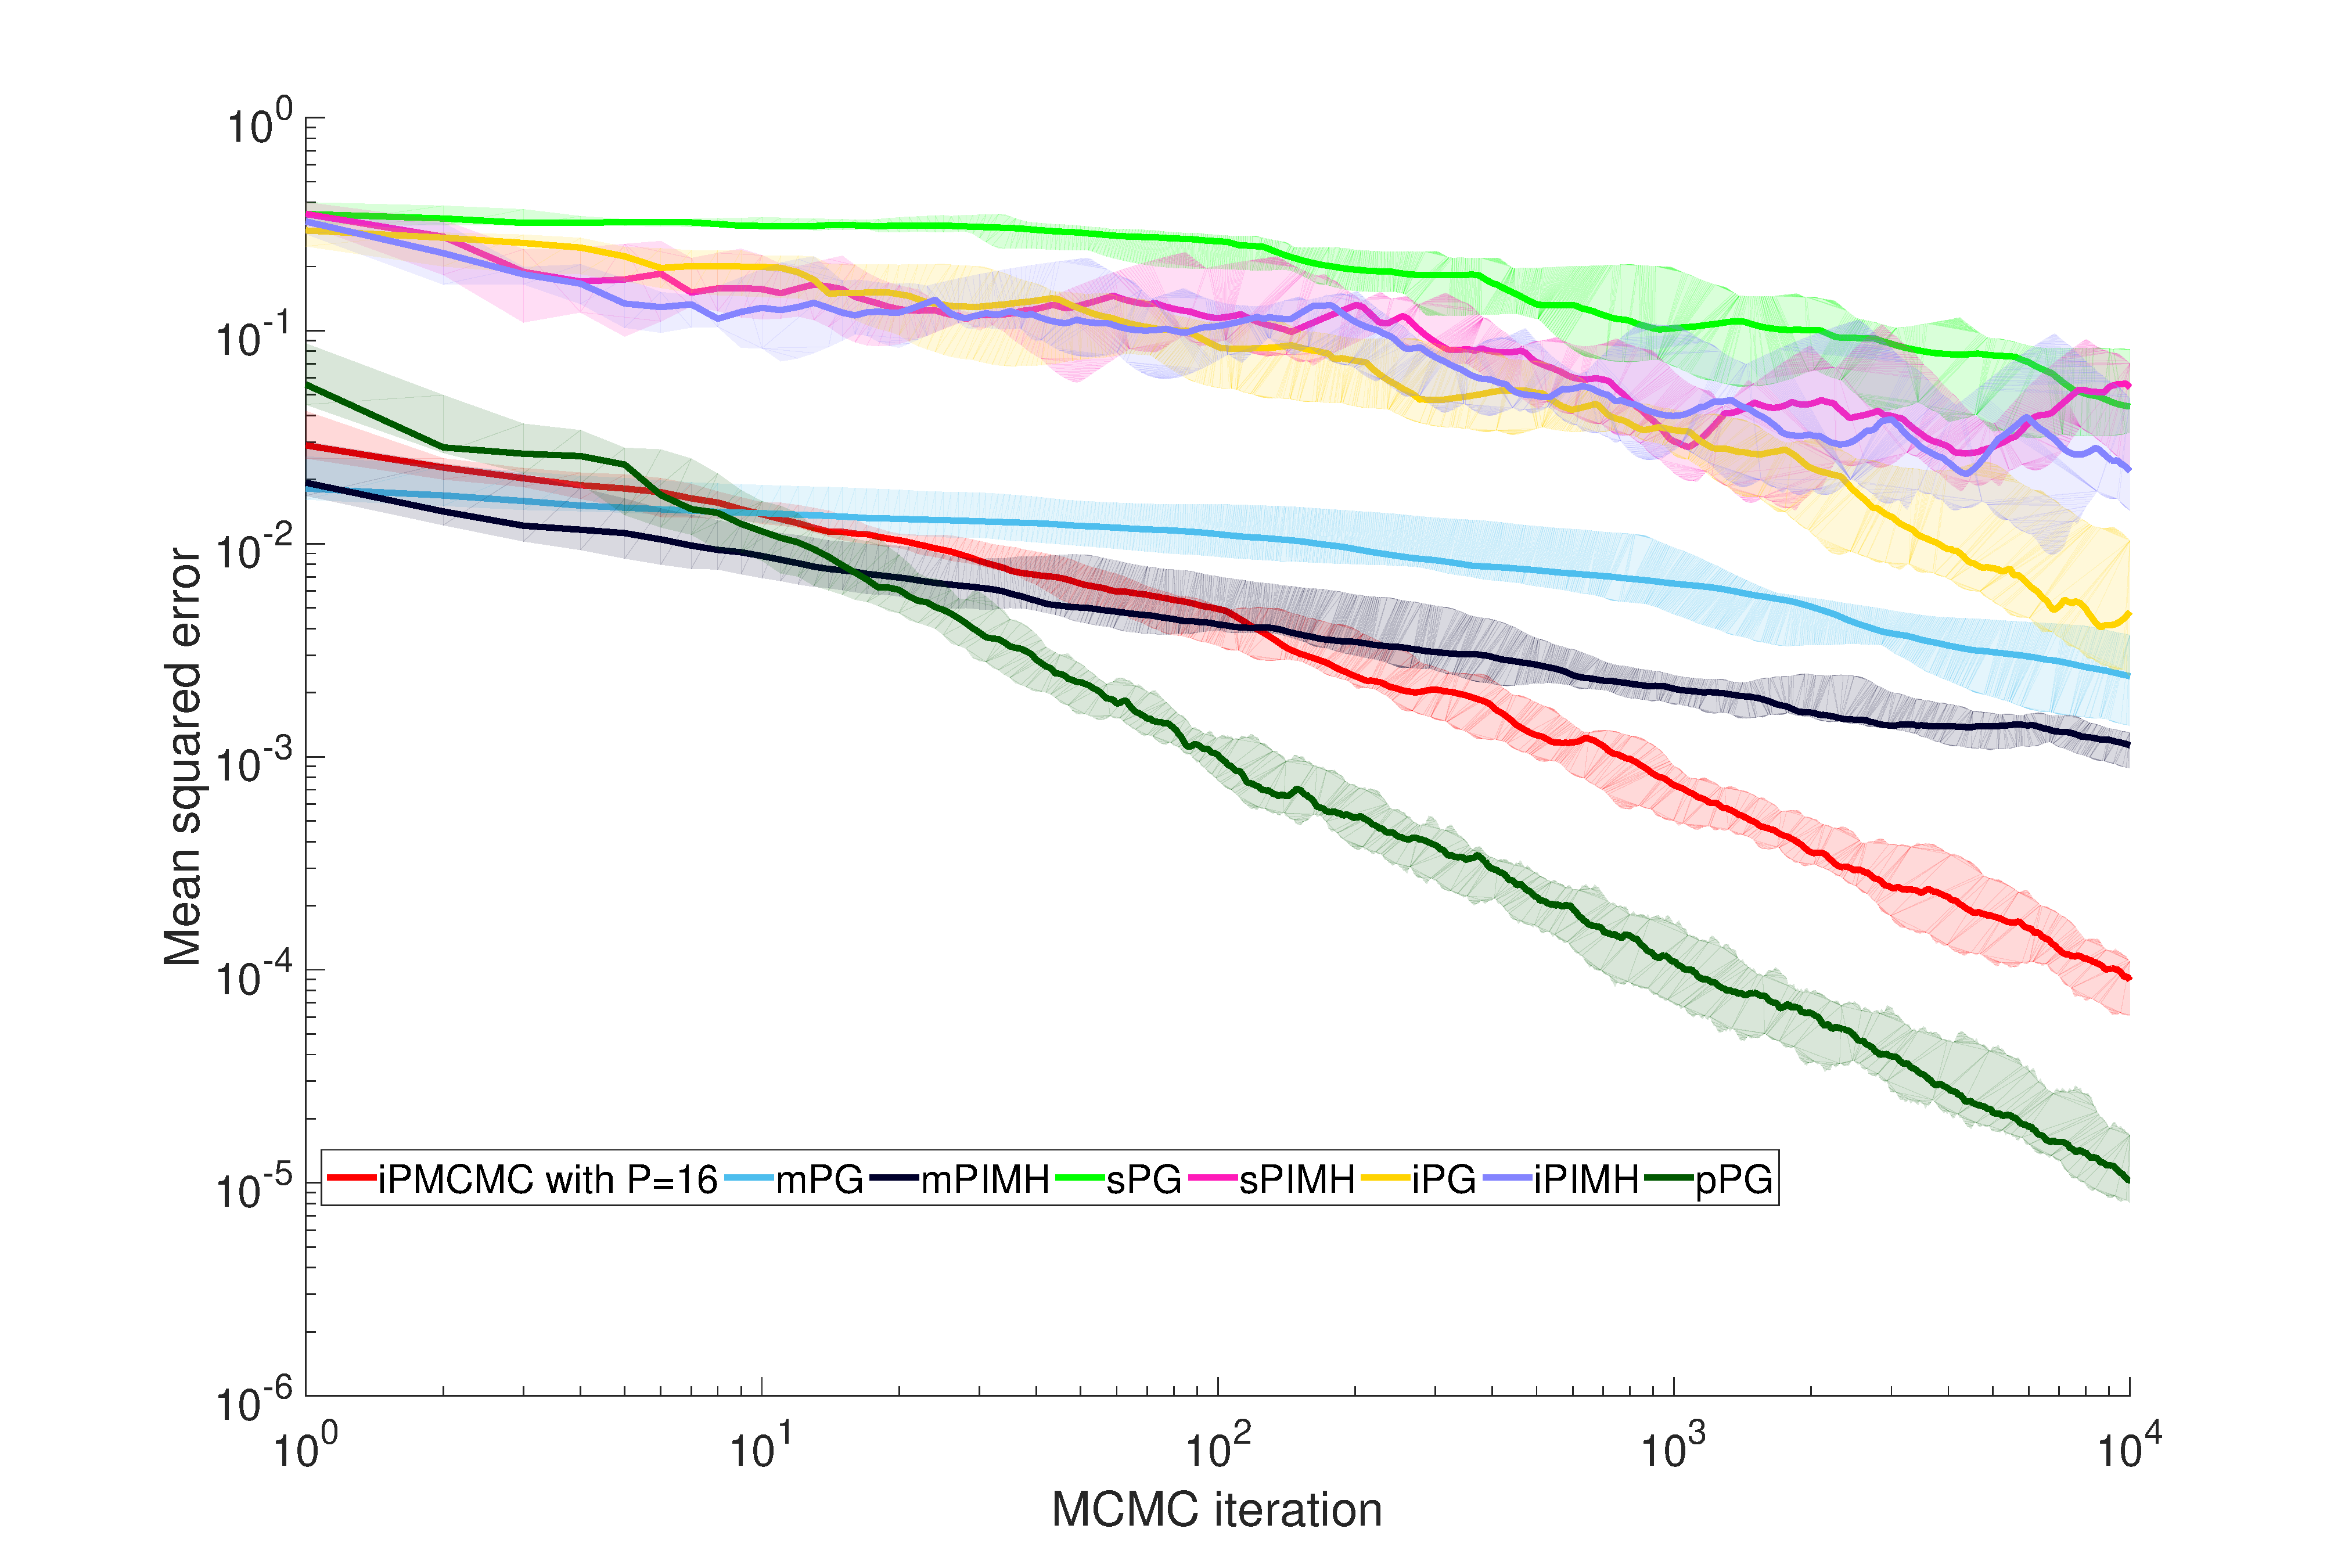
\includegraphics[width=1.1\textwidth,trim={2cm 0.7cm 2cm 0},clip]{mean_conv_series_lss}}
		\caption{Convergence in mean}
		\label{fig:supp-mean_series_conv}
	\end{subfigure}
	~ %add desired spacing between images, e. g. ~, \quad, \qquad, \hfill etc. 
	%(or a blank line to force the subfigure onto a new line)
	\begin{subfigure}[t]{0.49\textwidth}
		\makebox[\textwidth][l]{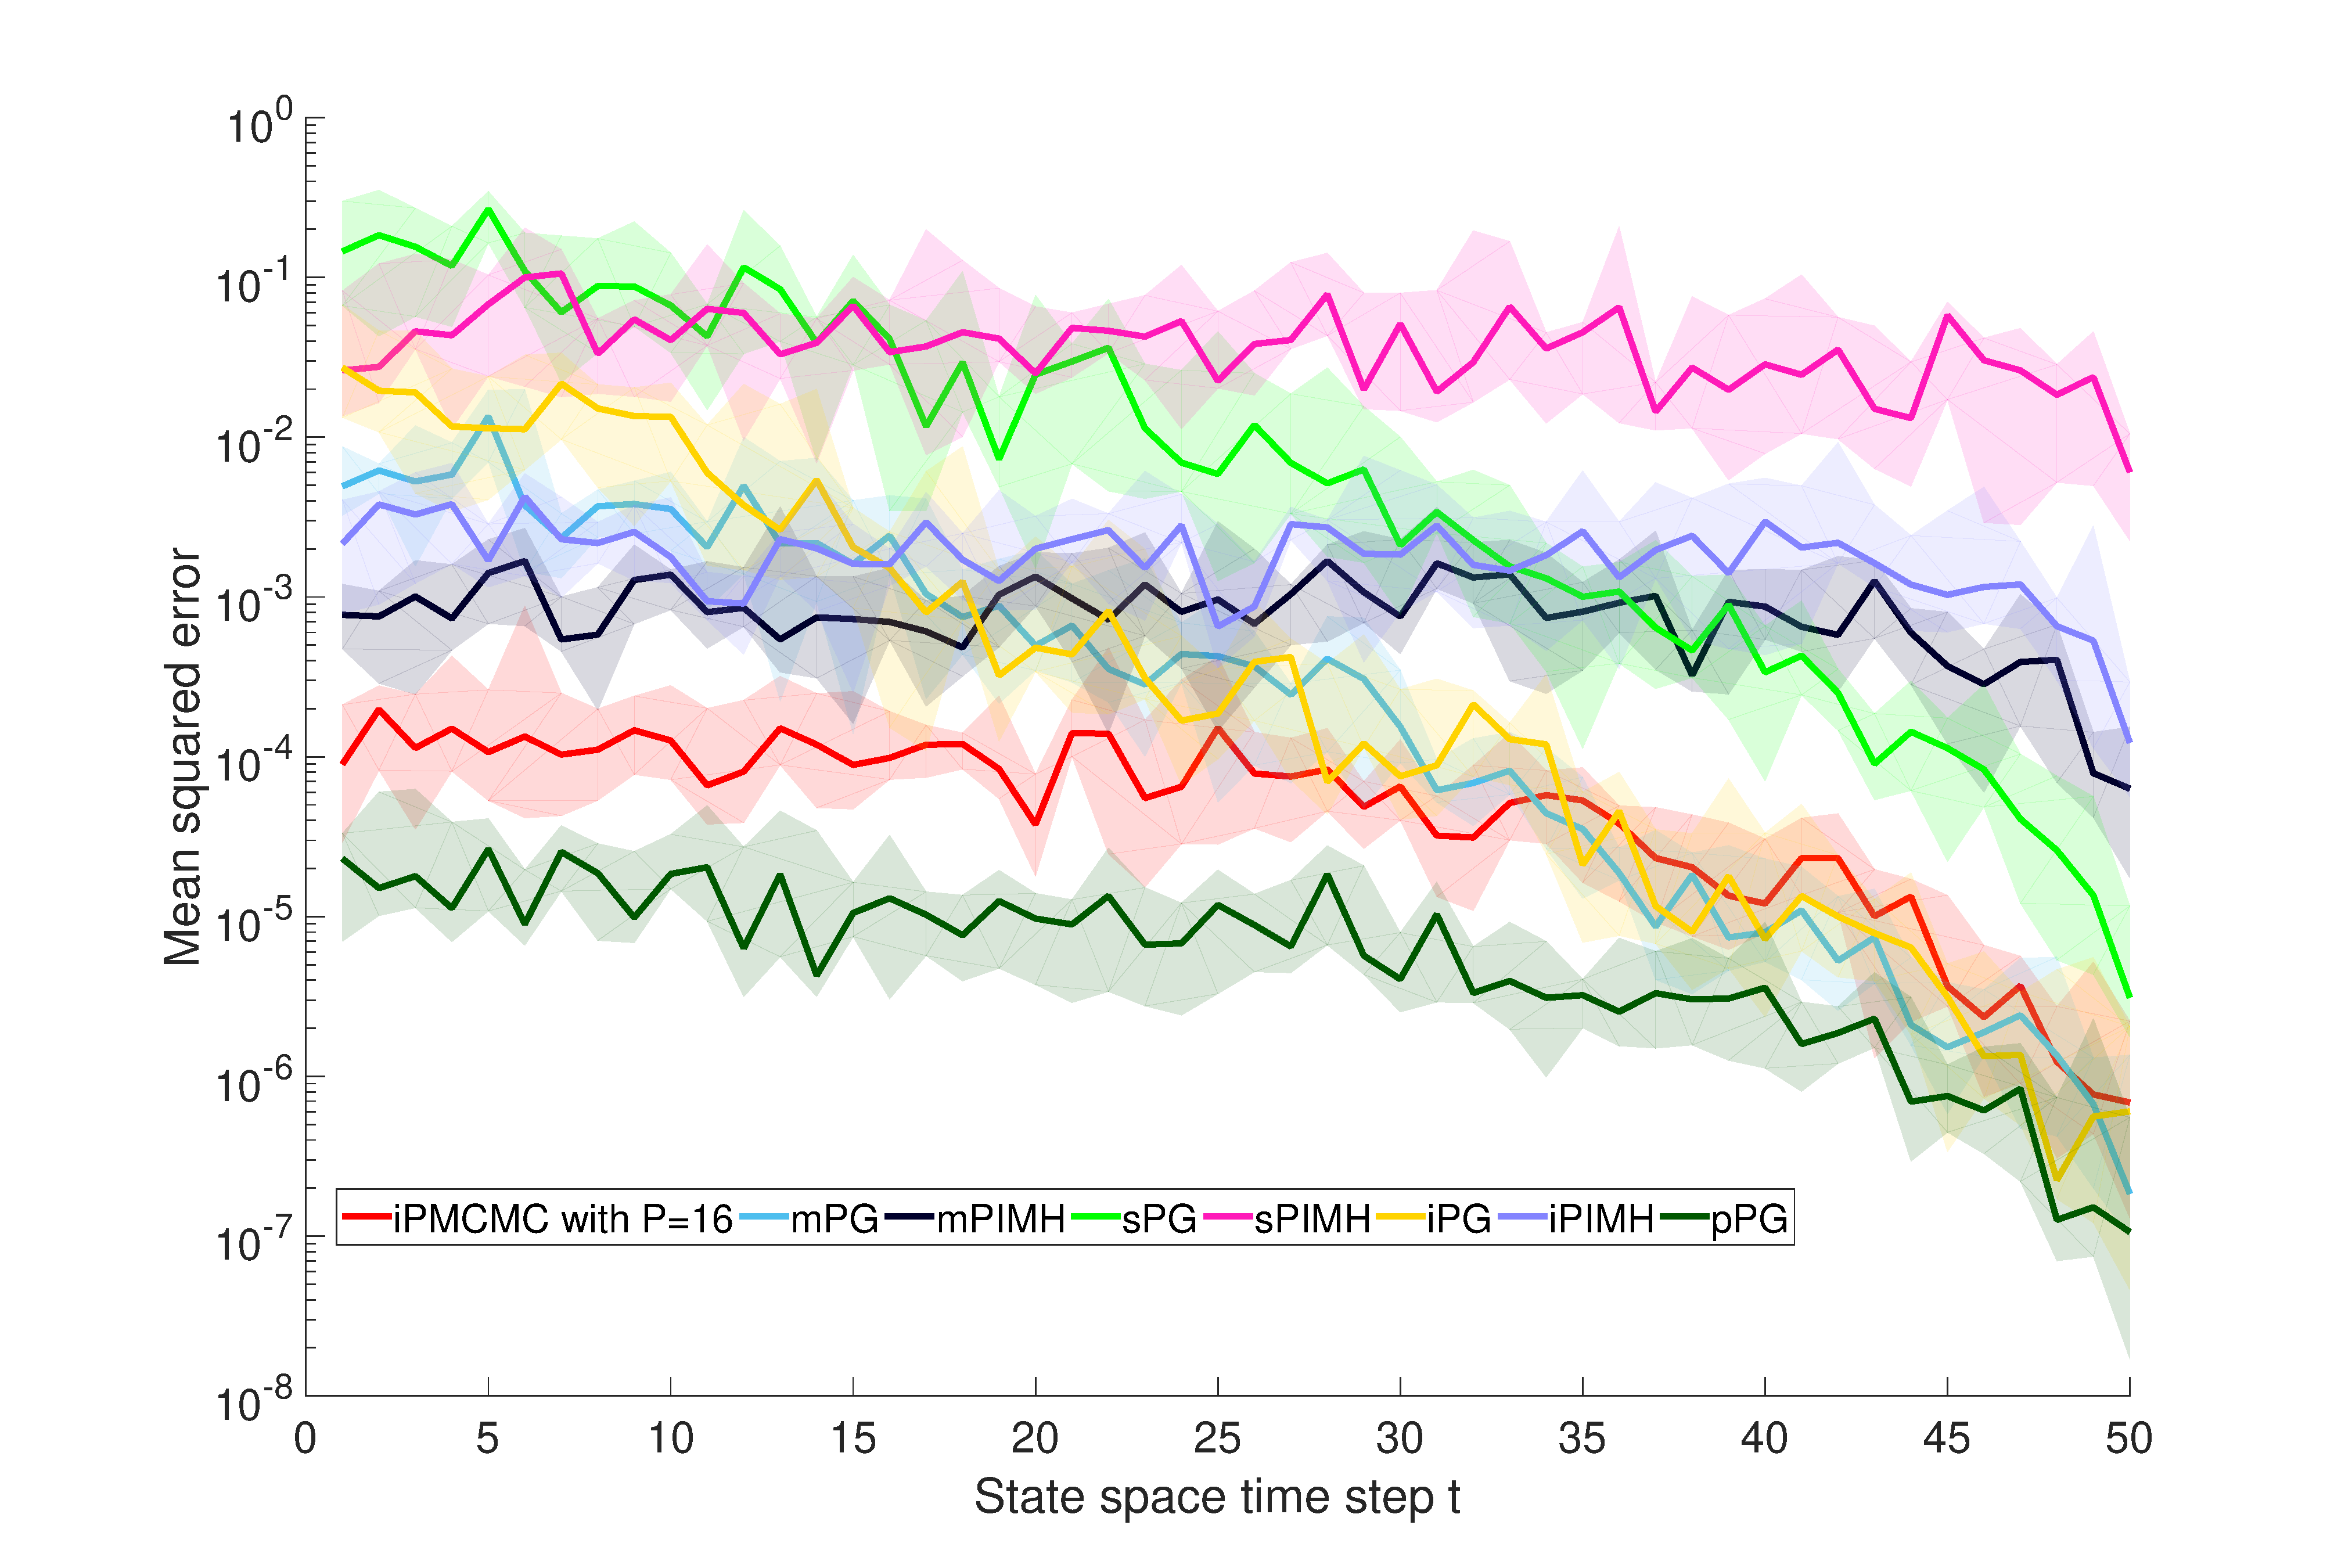
\includegraphics[width=1.1\textwidth,trim={4cm 0 5cm 0},clip]{mean_pos_series_lss}}
		\caption{Final error in mean}
		\label{fig:supp-mean_series_pos}
	\end{subfigure}
	
	\begin{subfigure}[t]{0.49\textwidth}
		\makebox[\textwidth][r]{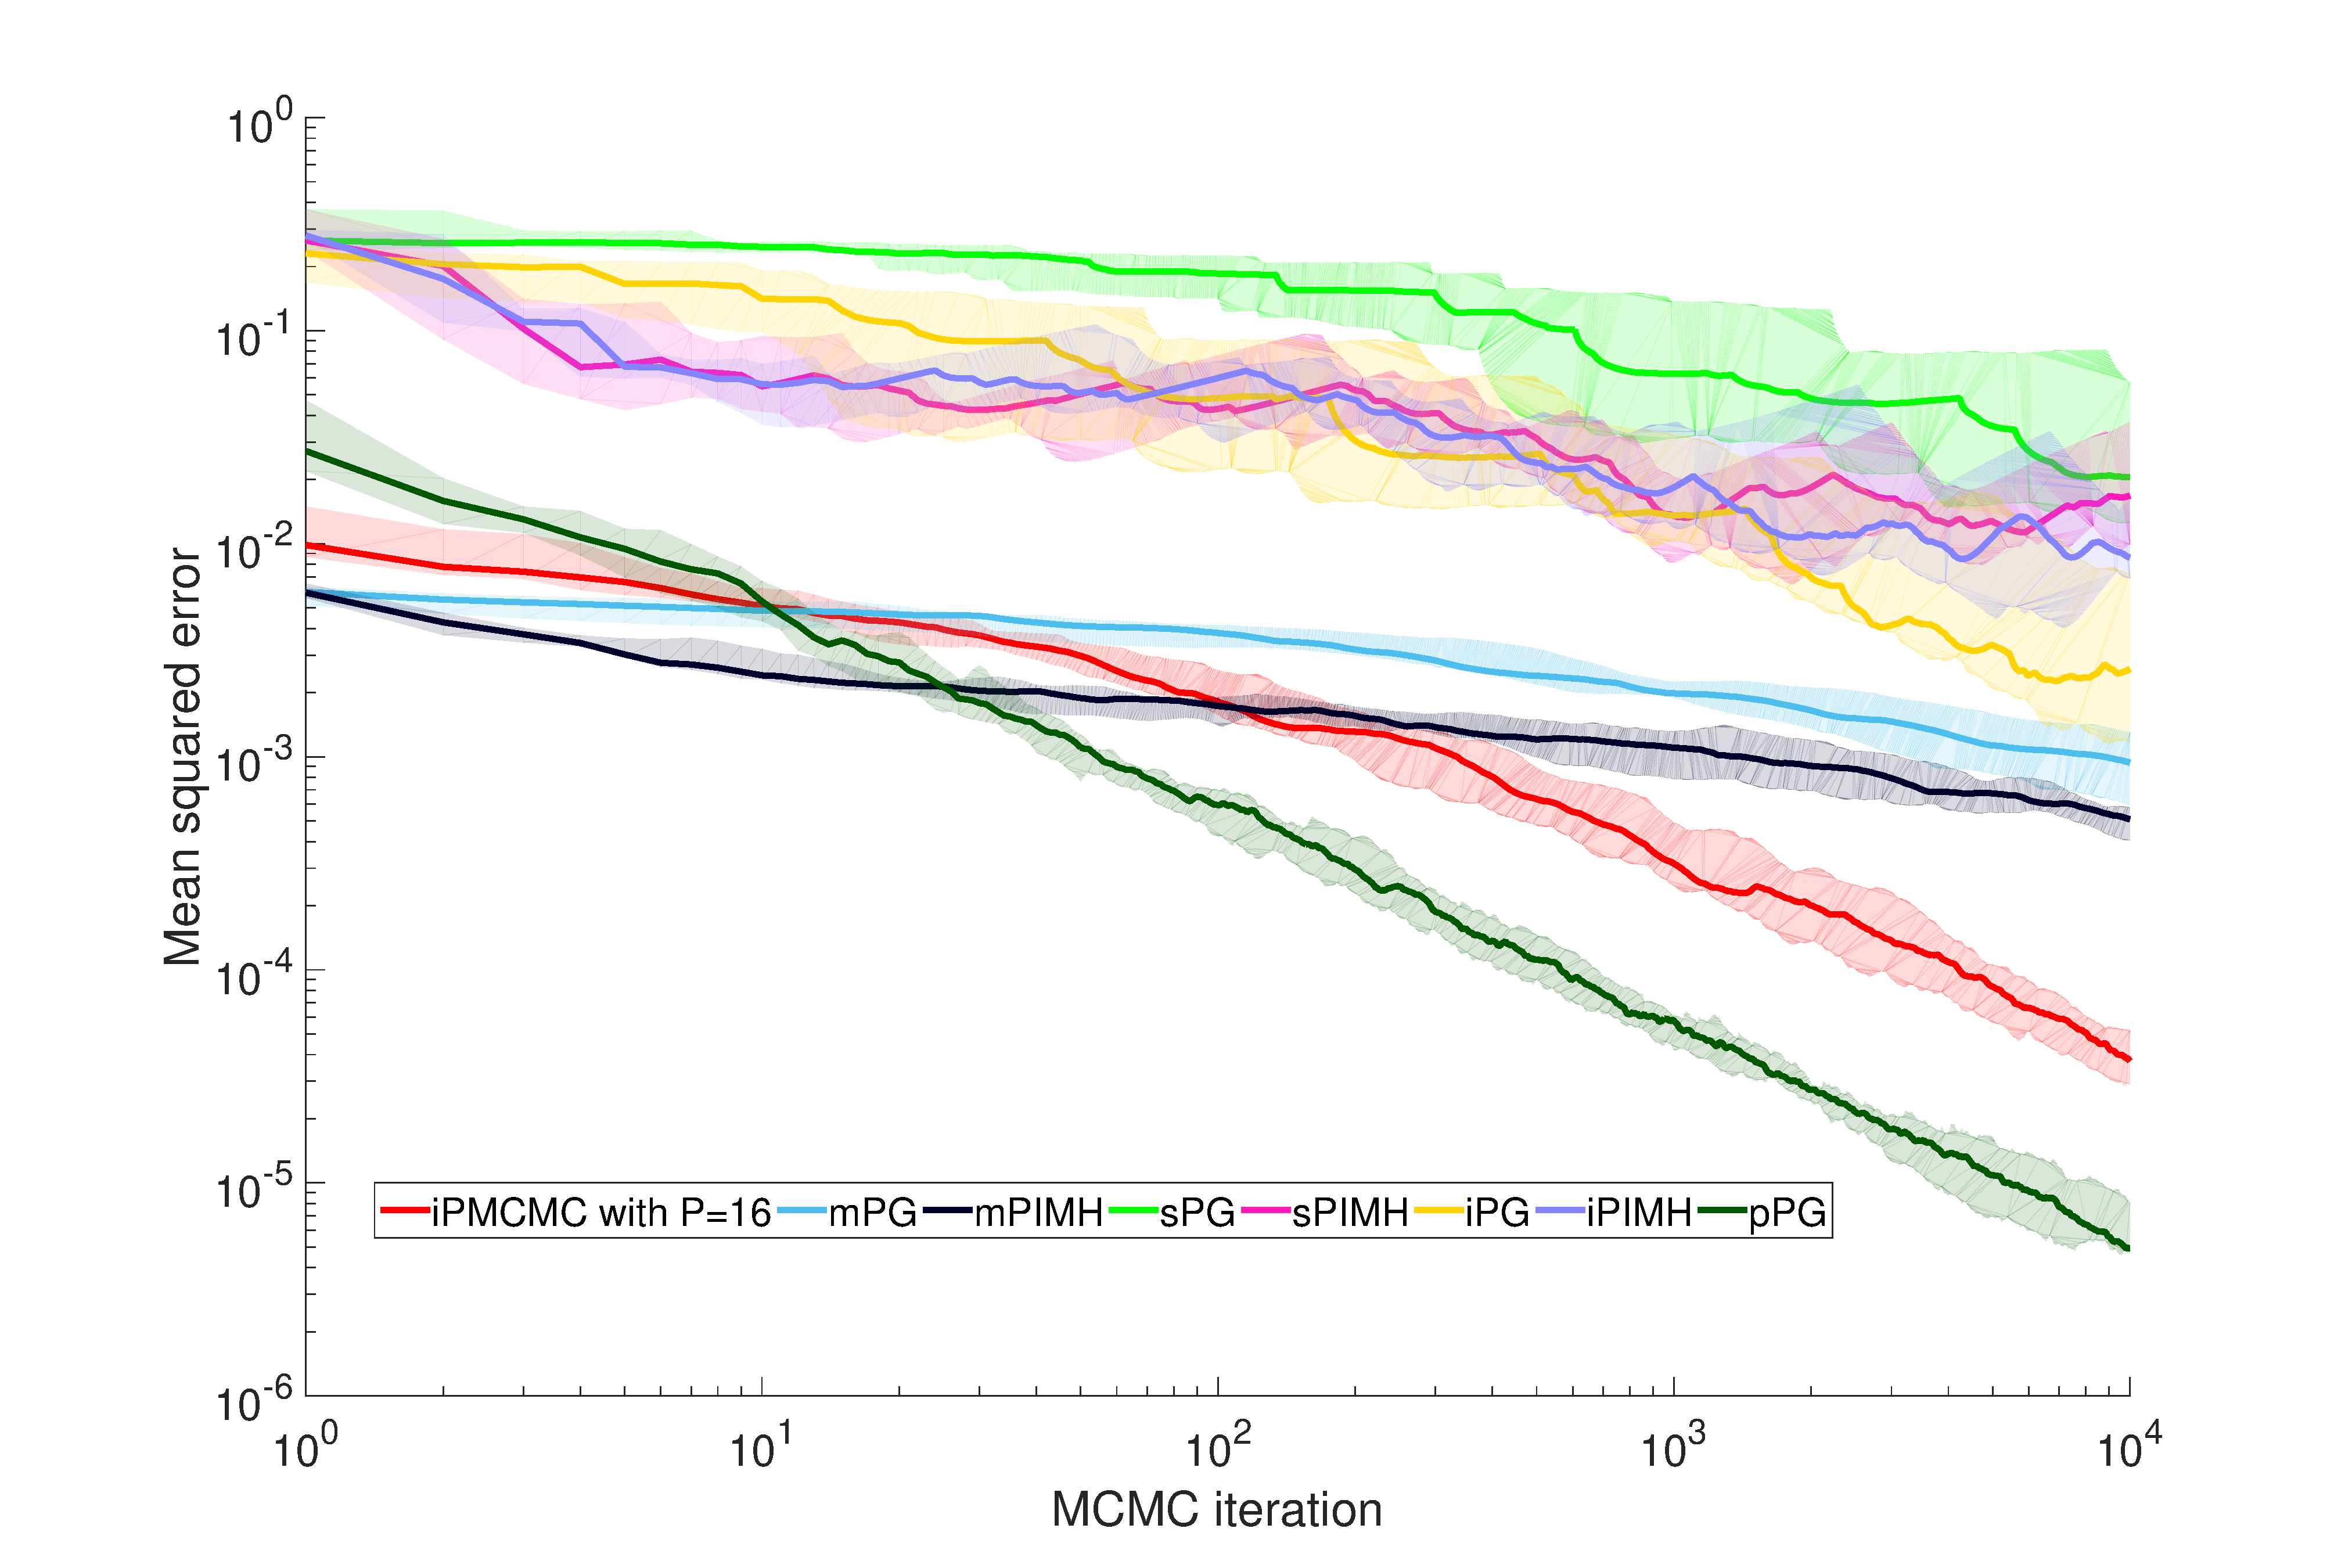
\includegraphics[width=1.1\textwidth,trim={2cm 0.7cm 2cm 0},clip]{std_conv_series_lss}}
		\caption{Convergence in standard deviation}
		\label{fig:supp-std_series_conv}
	\end{subfigure}
	~ %add desired spacing between images, e. g. ~, \quad, \qquad, \hfill etc. 
	%(or a blank line to force the subfigure onto a new line)
	\begin{subfigure}[t]{0.49\textwidth}
		\makebox[\textwidth][l]{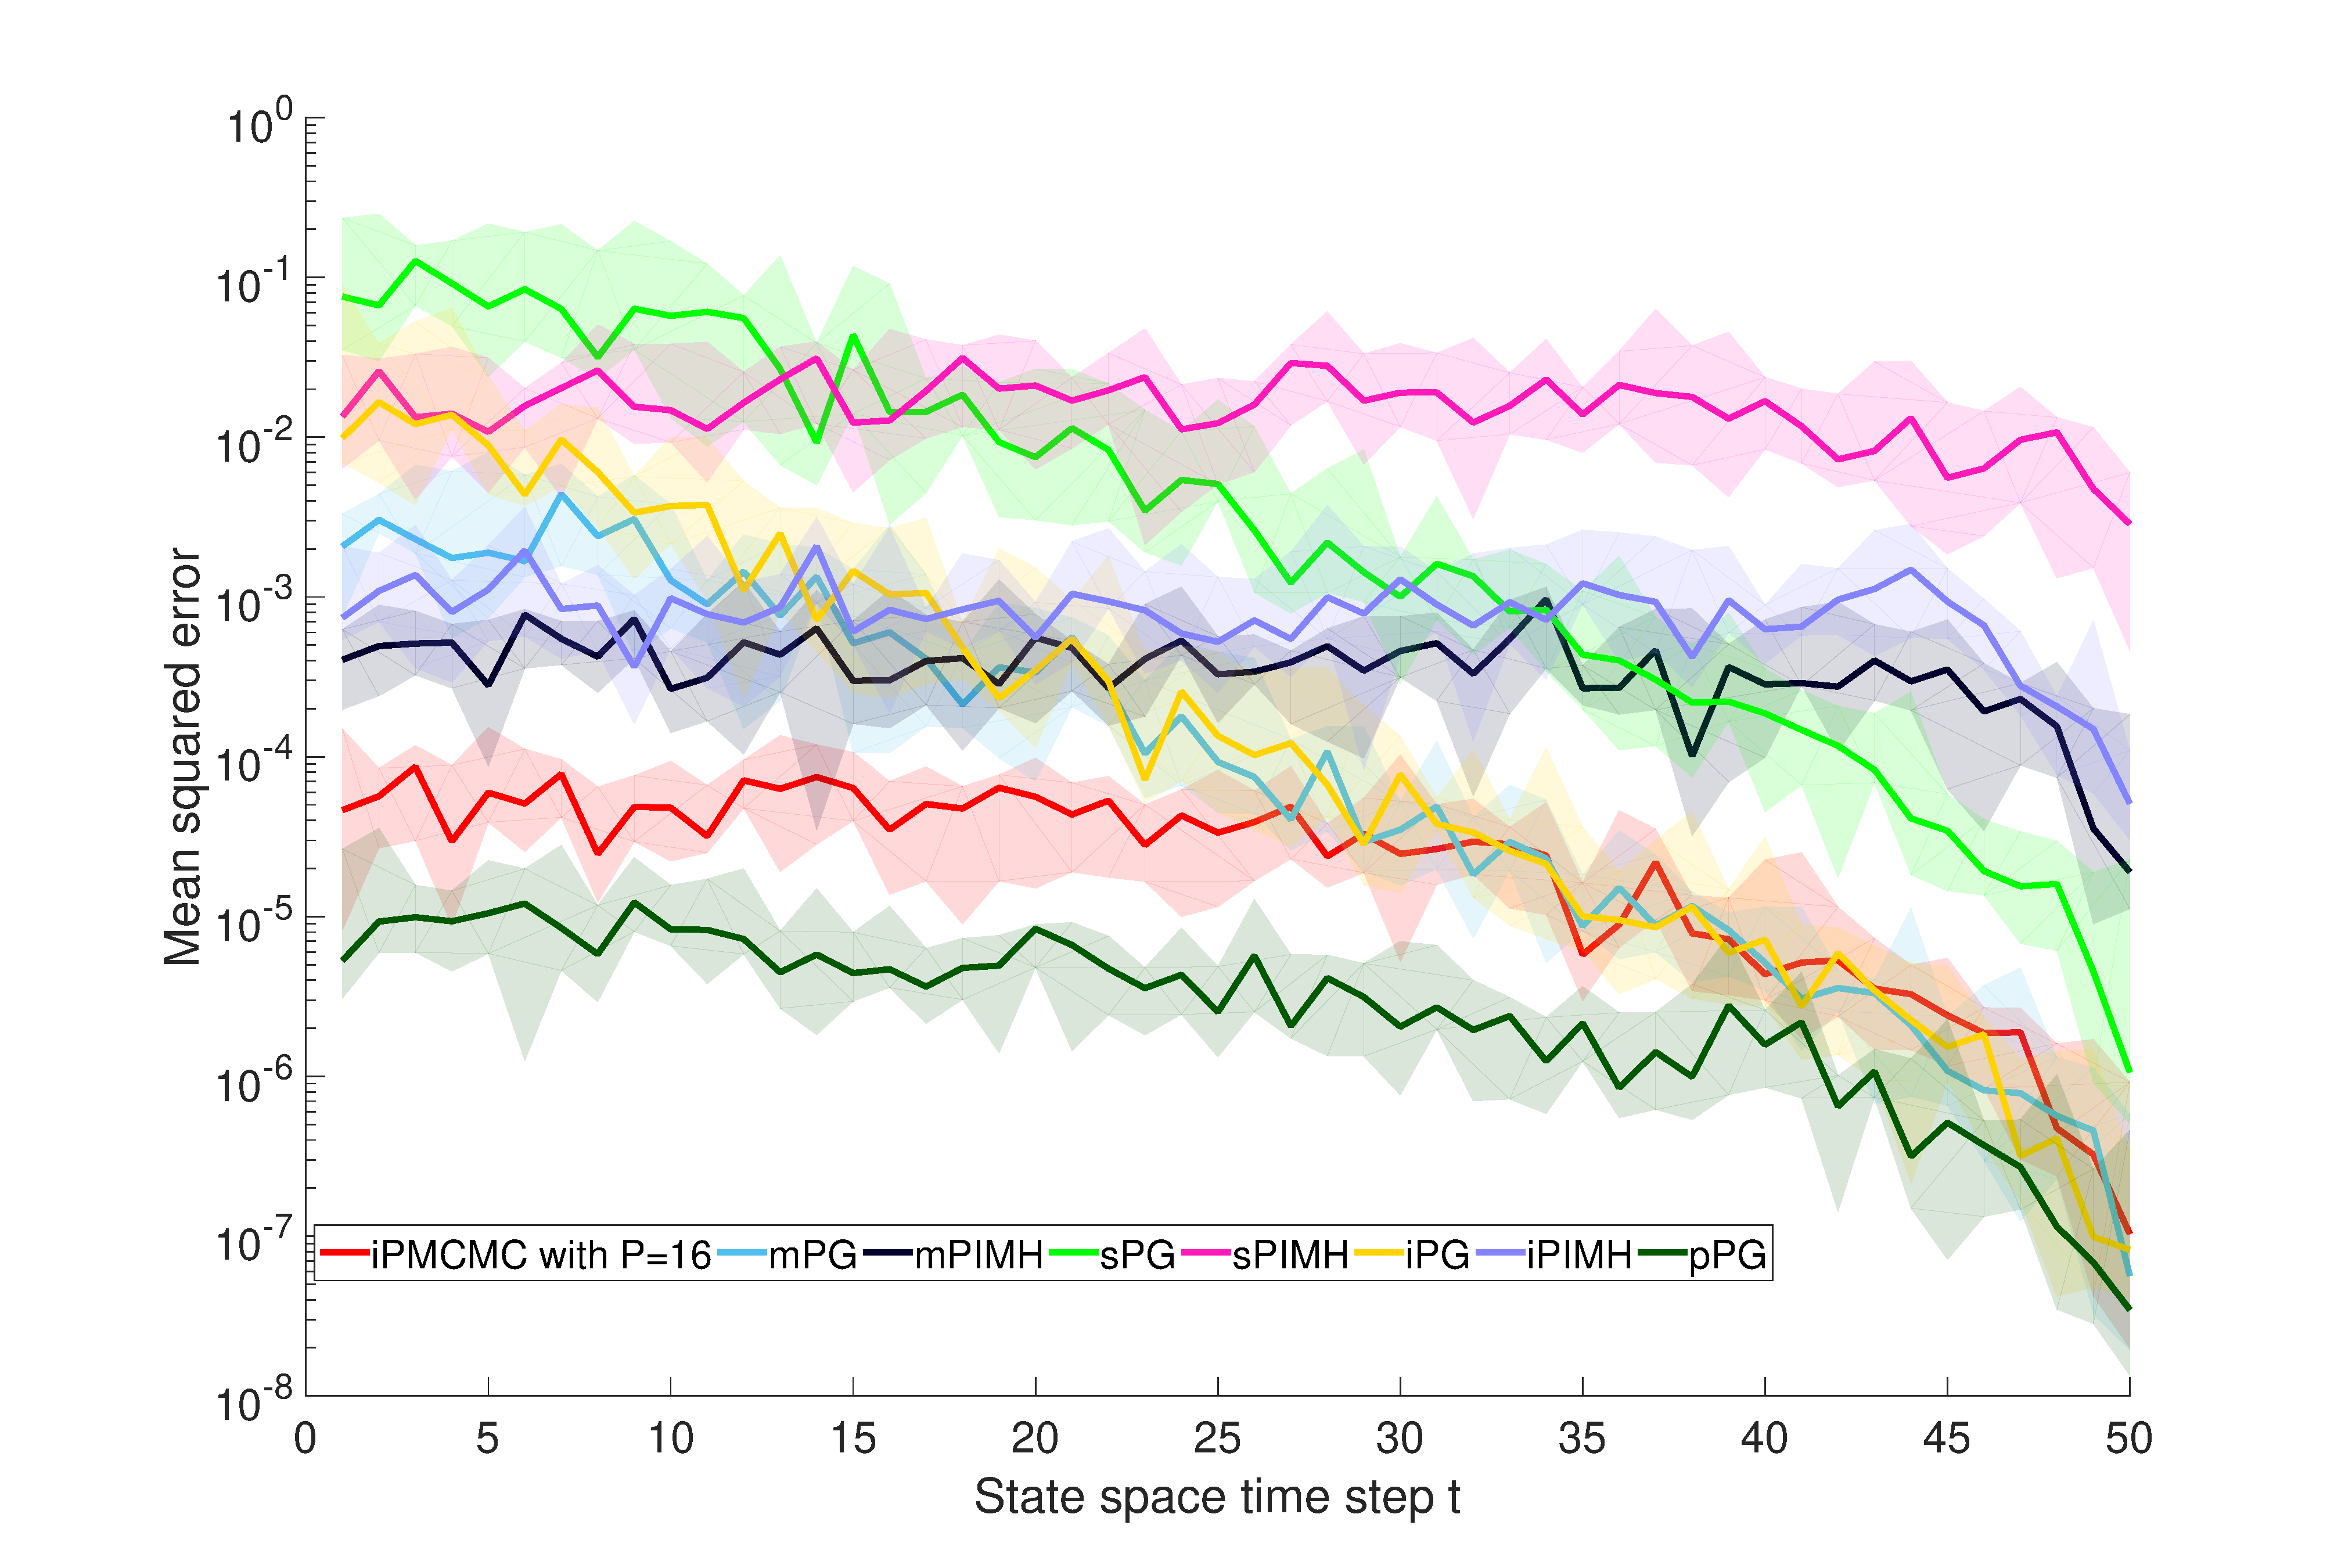
\includegraphics[width=1.1\textwidth,trim={4cm 0 5cm 0},clip]{std_pos_series_lss}}
		\caption{Final error in standard deviation}
		\label{fig:supp-std_series_pos}
	\end{subfigure}	
	
	\caption{Mean squared error in latent variable mean and standard deviation averaged of all dimensions of the LGSSM as a function of MCMC iteration (left) and position in the state sequence (right) for iPMCMC, mPG, mPIMH and a number of serialized variants.  Key for legends: sPG = single PG chain, sPIMH = single PIMH chain, iPG = single PG chain run 32 times longer, iPIMH = single PIMH chain run 32 times longer and pPG = single PG with 32 times more particles.  For visualization purposes, the chains with extra iterations have had the number of MCMC iterations normalized by 32 so that the different methods represent equivalent total computational budget. \label{fig:supp-series_error_lss}}
\end{figure*}

\begin{figure*}[p]
	\centering
	\begin{subfigure}[t]{0.49\textwidth}
		\makebox[\textwidth][r]{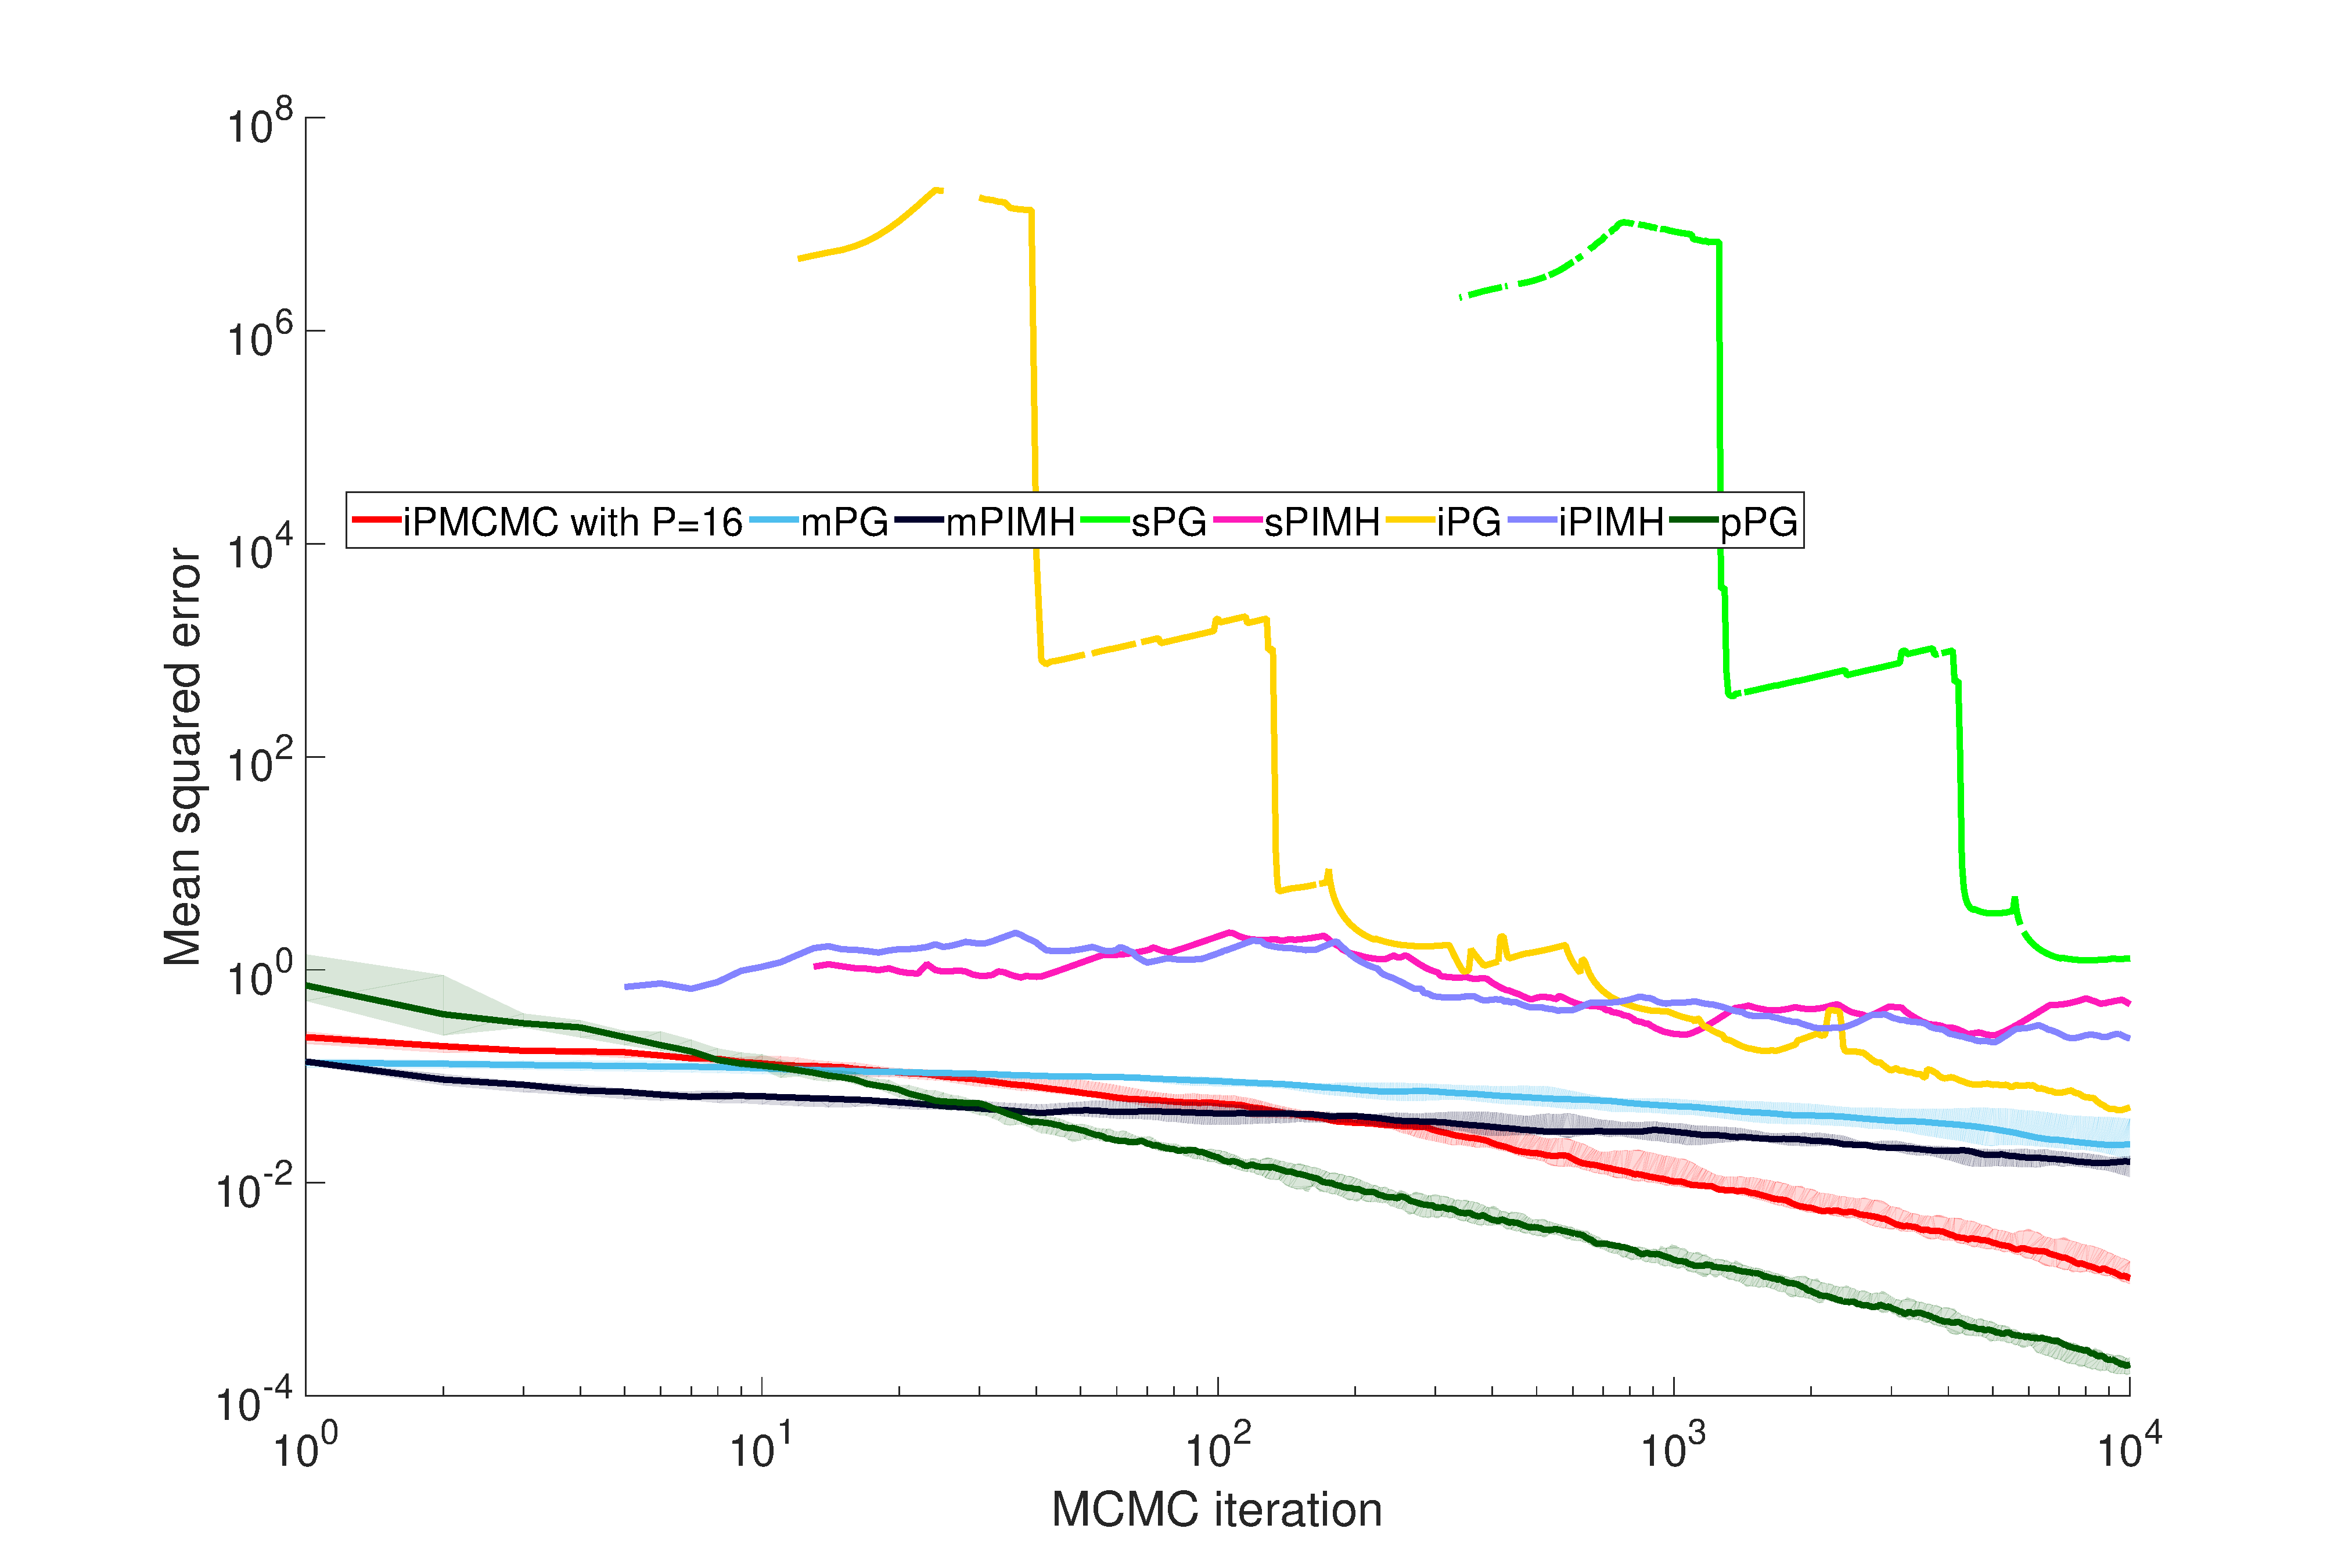
\includegraphics[width=1.1\textwidth,trim={4cm 0 5cm 0},clip]{skewness_conv_series_lss}}
		\caption{Convergence in skewness}
		\label{fig:supp-ske_series_conv}
	\end{subfigure}
	~ %add desired spacing between images, e. g. ~, \quad, \qquad, \hfill etc. 
	%(or a blank line to force the subfigure onto a new line)
	\begin{subfigure}[t]{0.49\textwidth}
		\makebox[\textwidth][l]{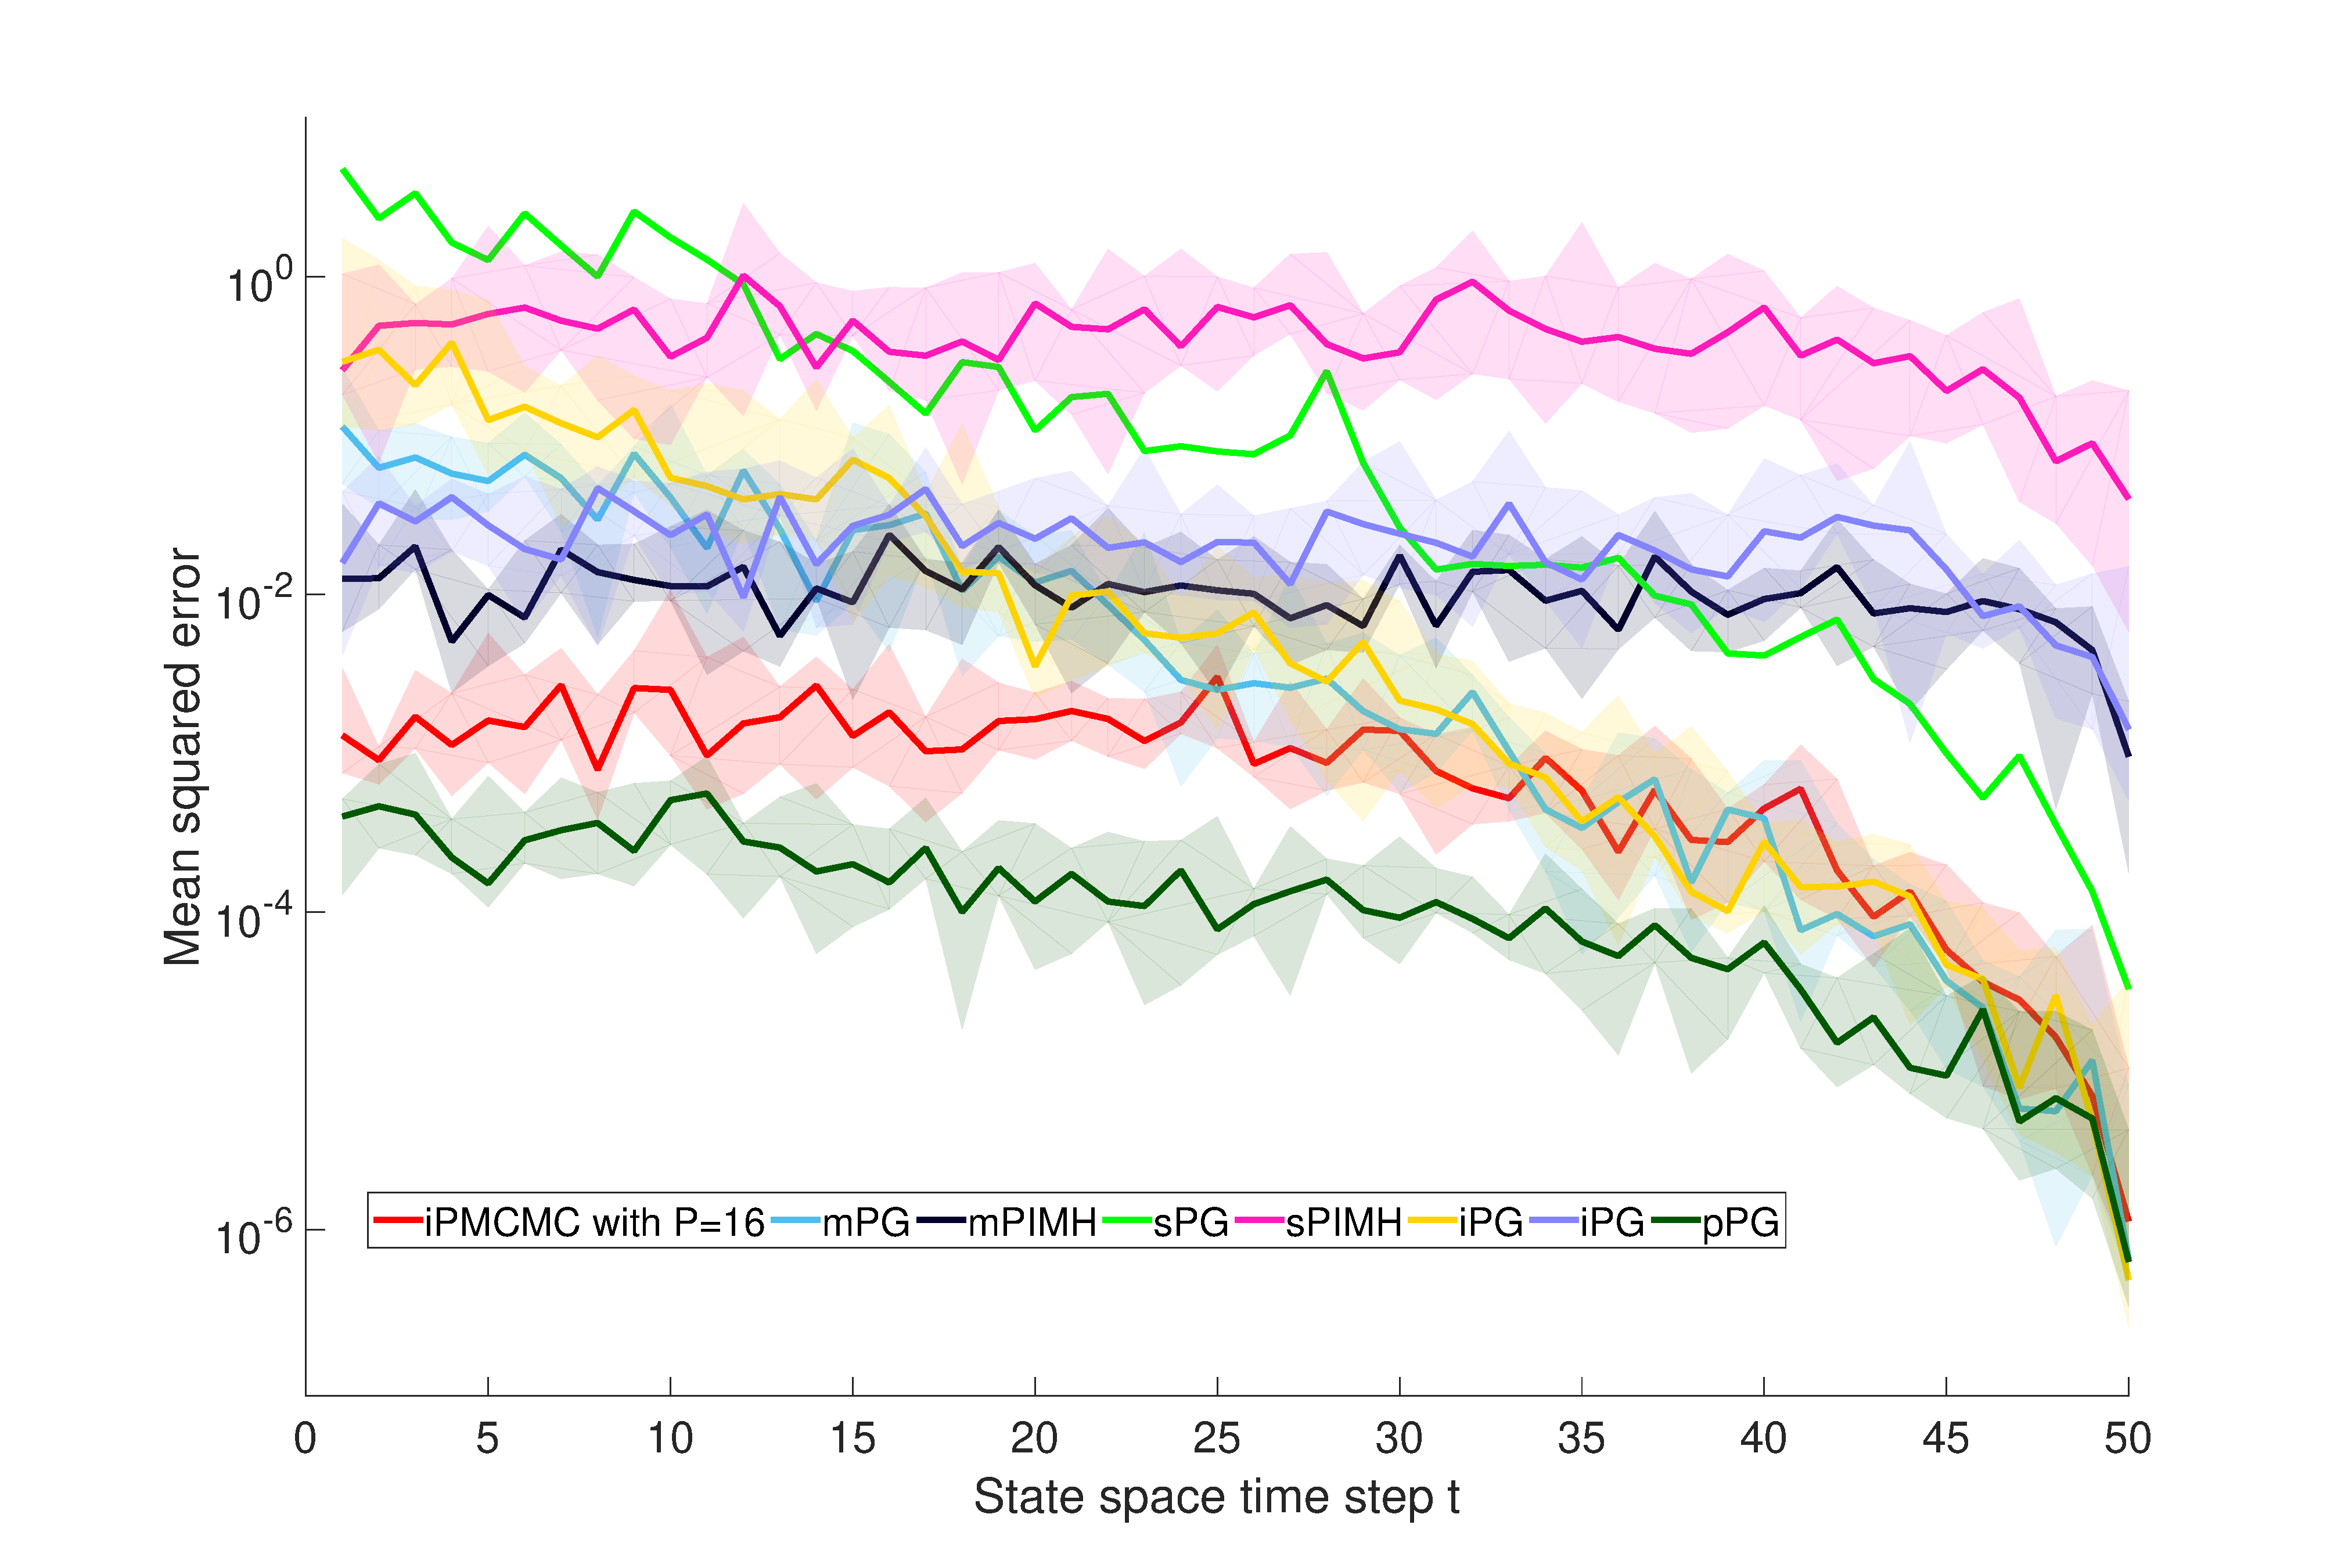
\includegraphics[width=1.1\textwidth,trim={4cm 0 5cm 0},clip]{skewness_pos_series_lss}}
		\caption{Final error in skewness}
		\label{fig:supp-ske_series_pos}
	\end{subfigure}	
	
	\begin{subfigure}[t]{0.49\textwidth}
		\makebox[\textwidth][r]{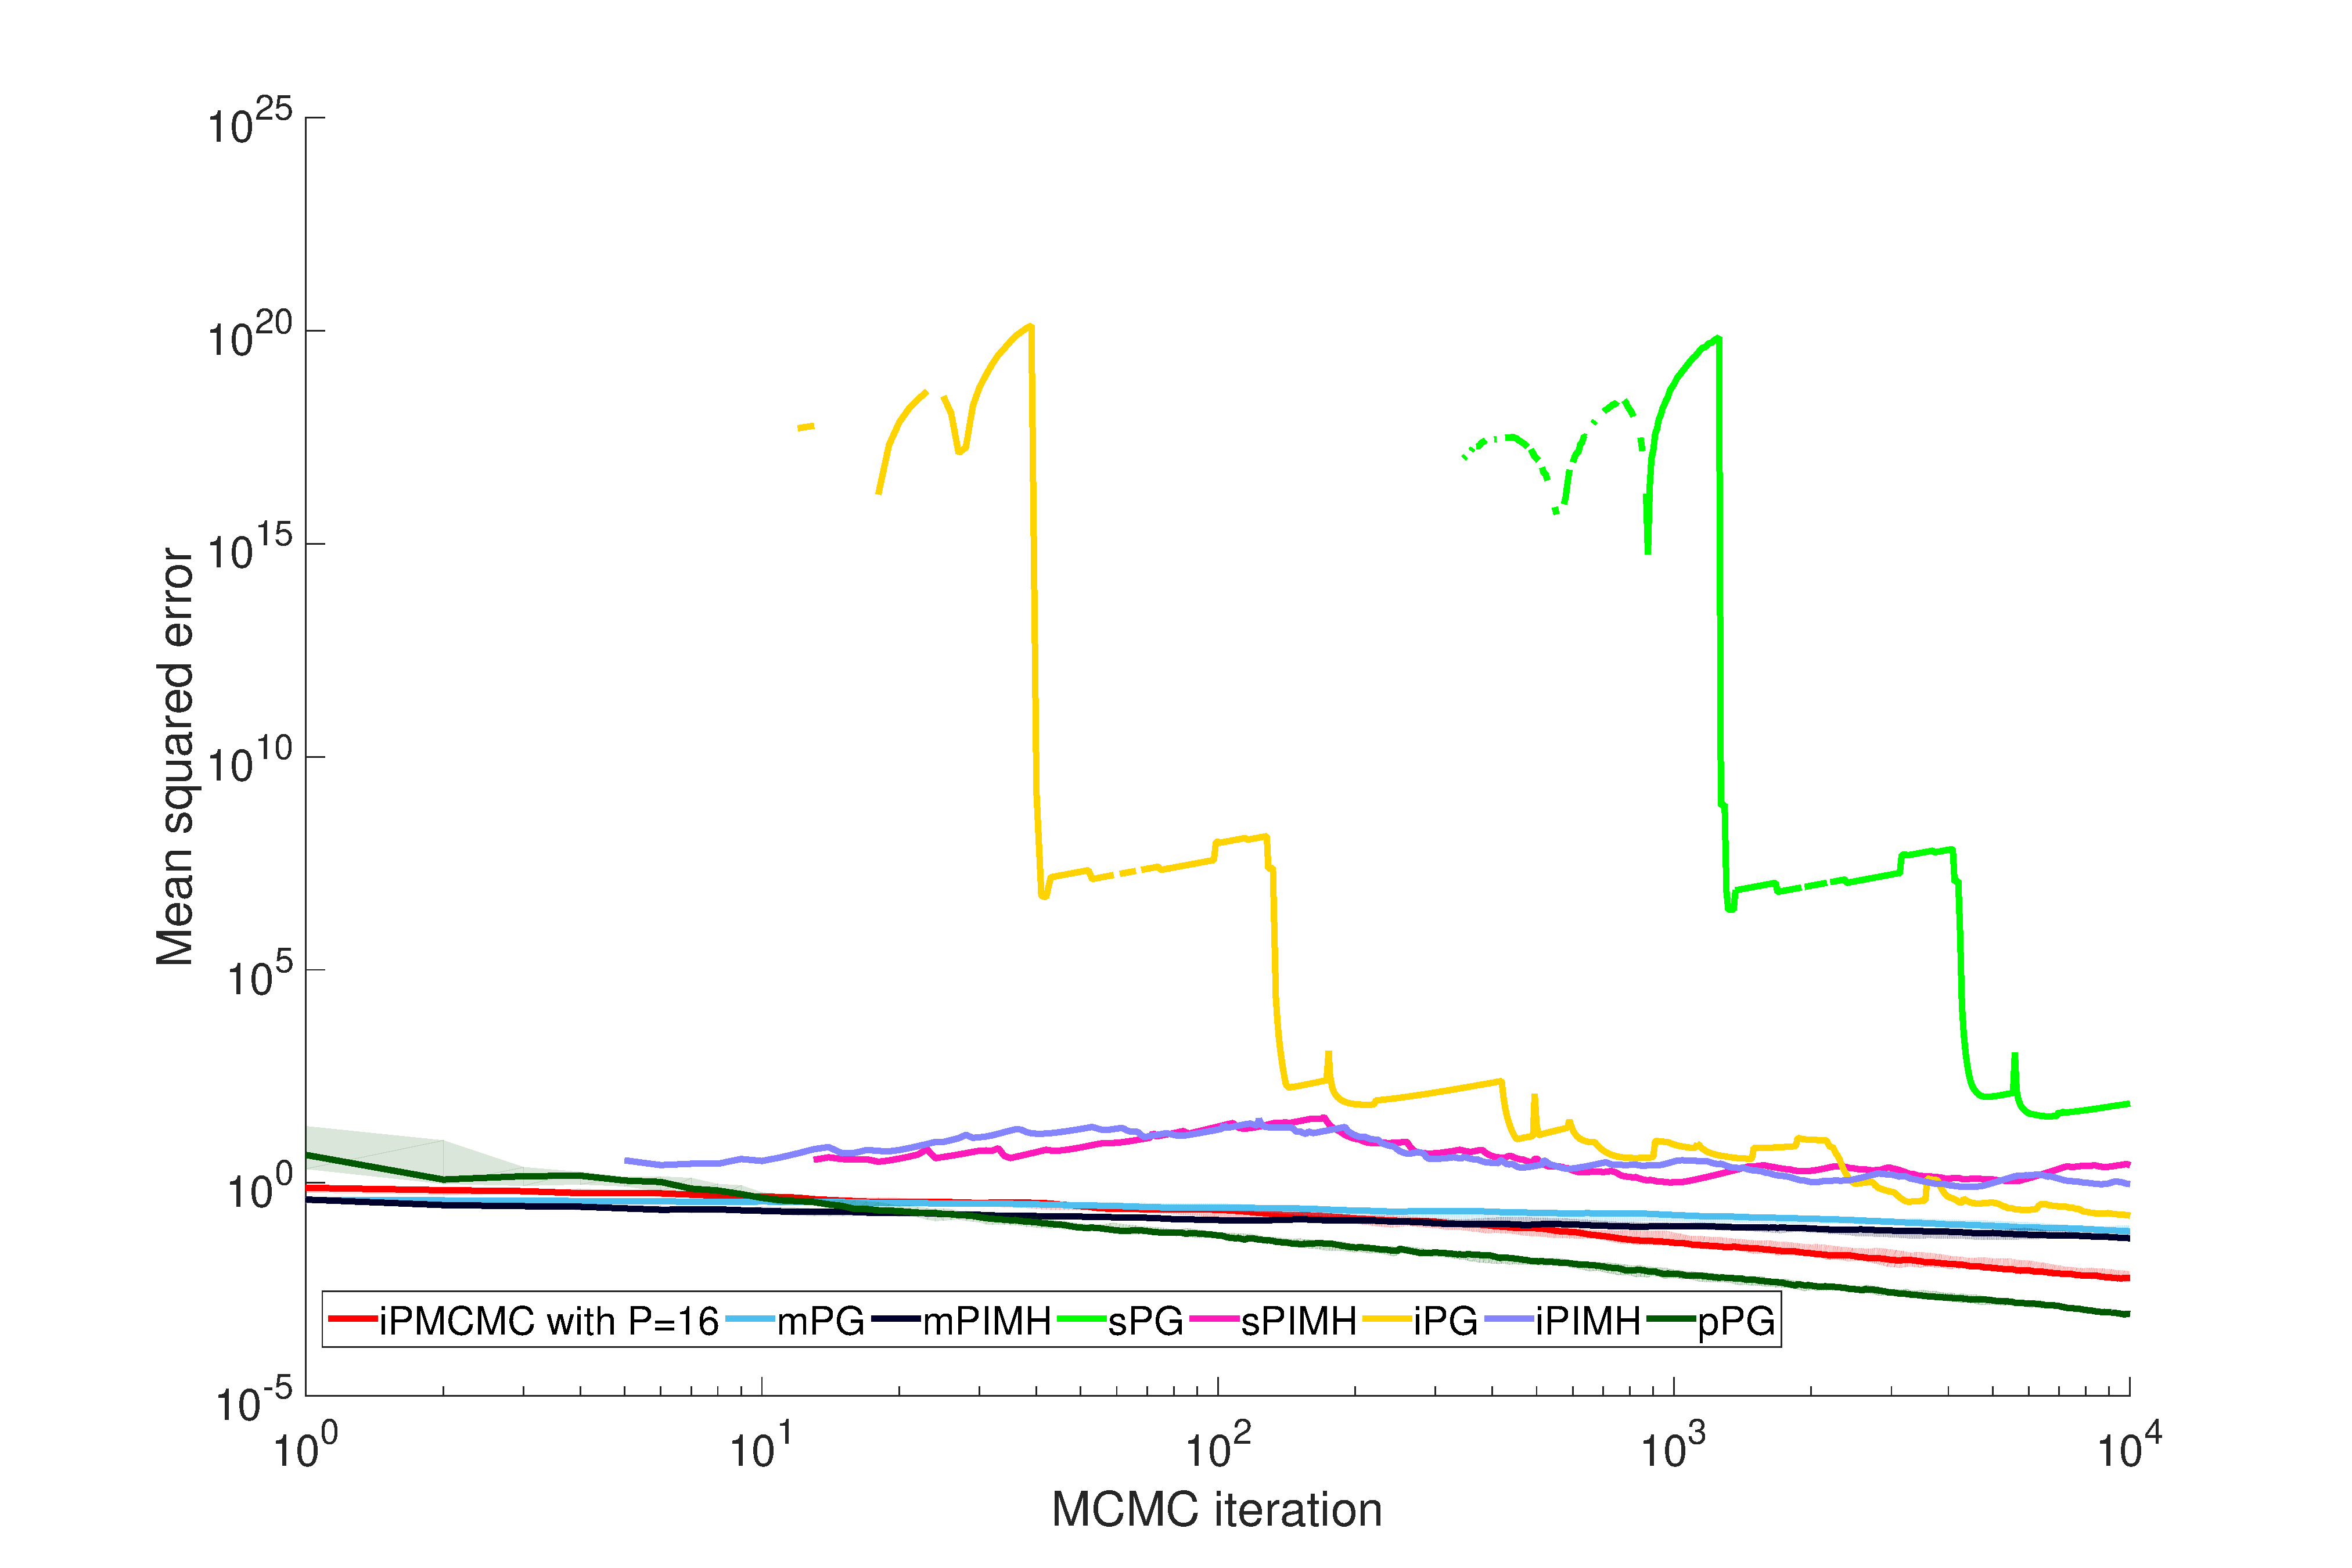
\includegraphics[width=1.1\textwidth,trim={4cm 0 5cm 0},clip]{kurtosis_conv_series_lss}}
		\caption{Convergence in kurtosis}
		\label{fig:supp-kurt_series_conv}
	\end{subfigure}
	~ %add desired spacing between images, e. g. ~, \quad, \qquad, \hfill etc. 
	%(or a blank line to force the subfigure onto a new line)
	\begin{subfigure}[t]{0.49\textwidth}
		\makebox[\textwidth][l]{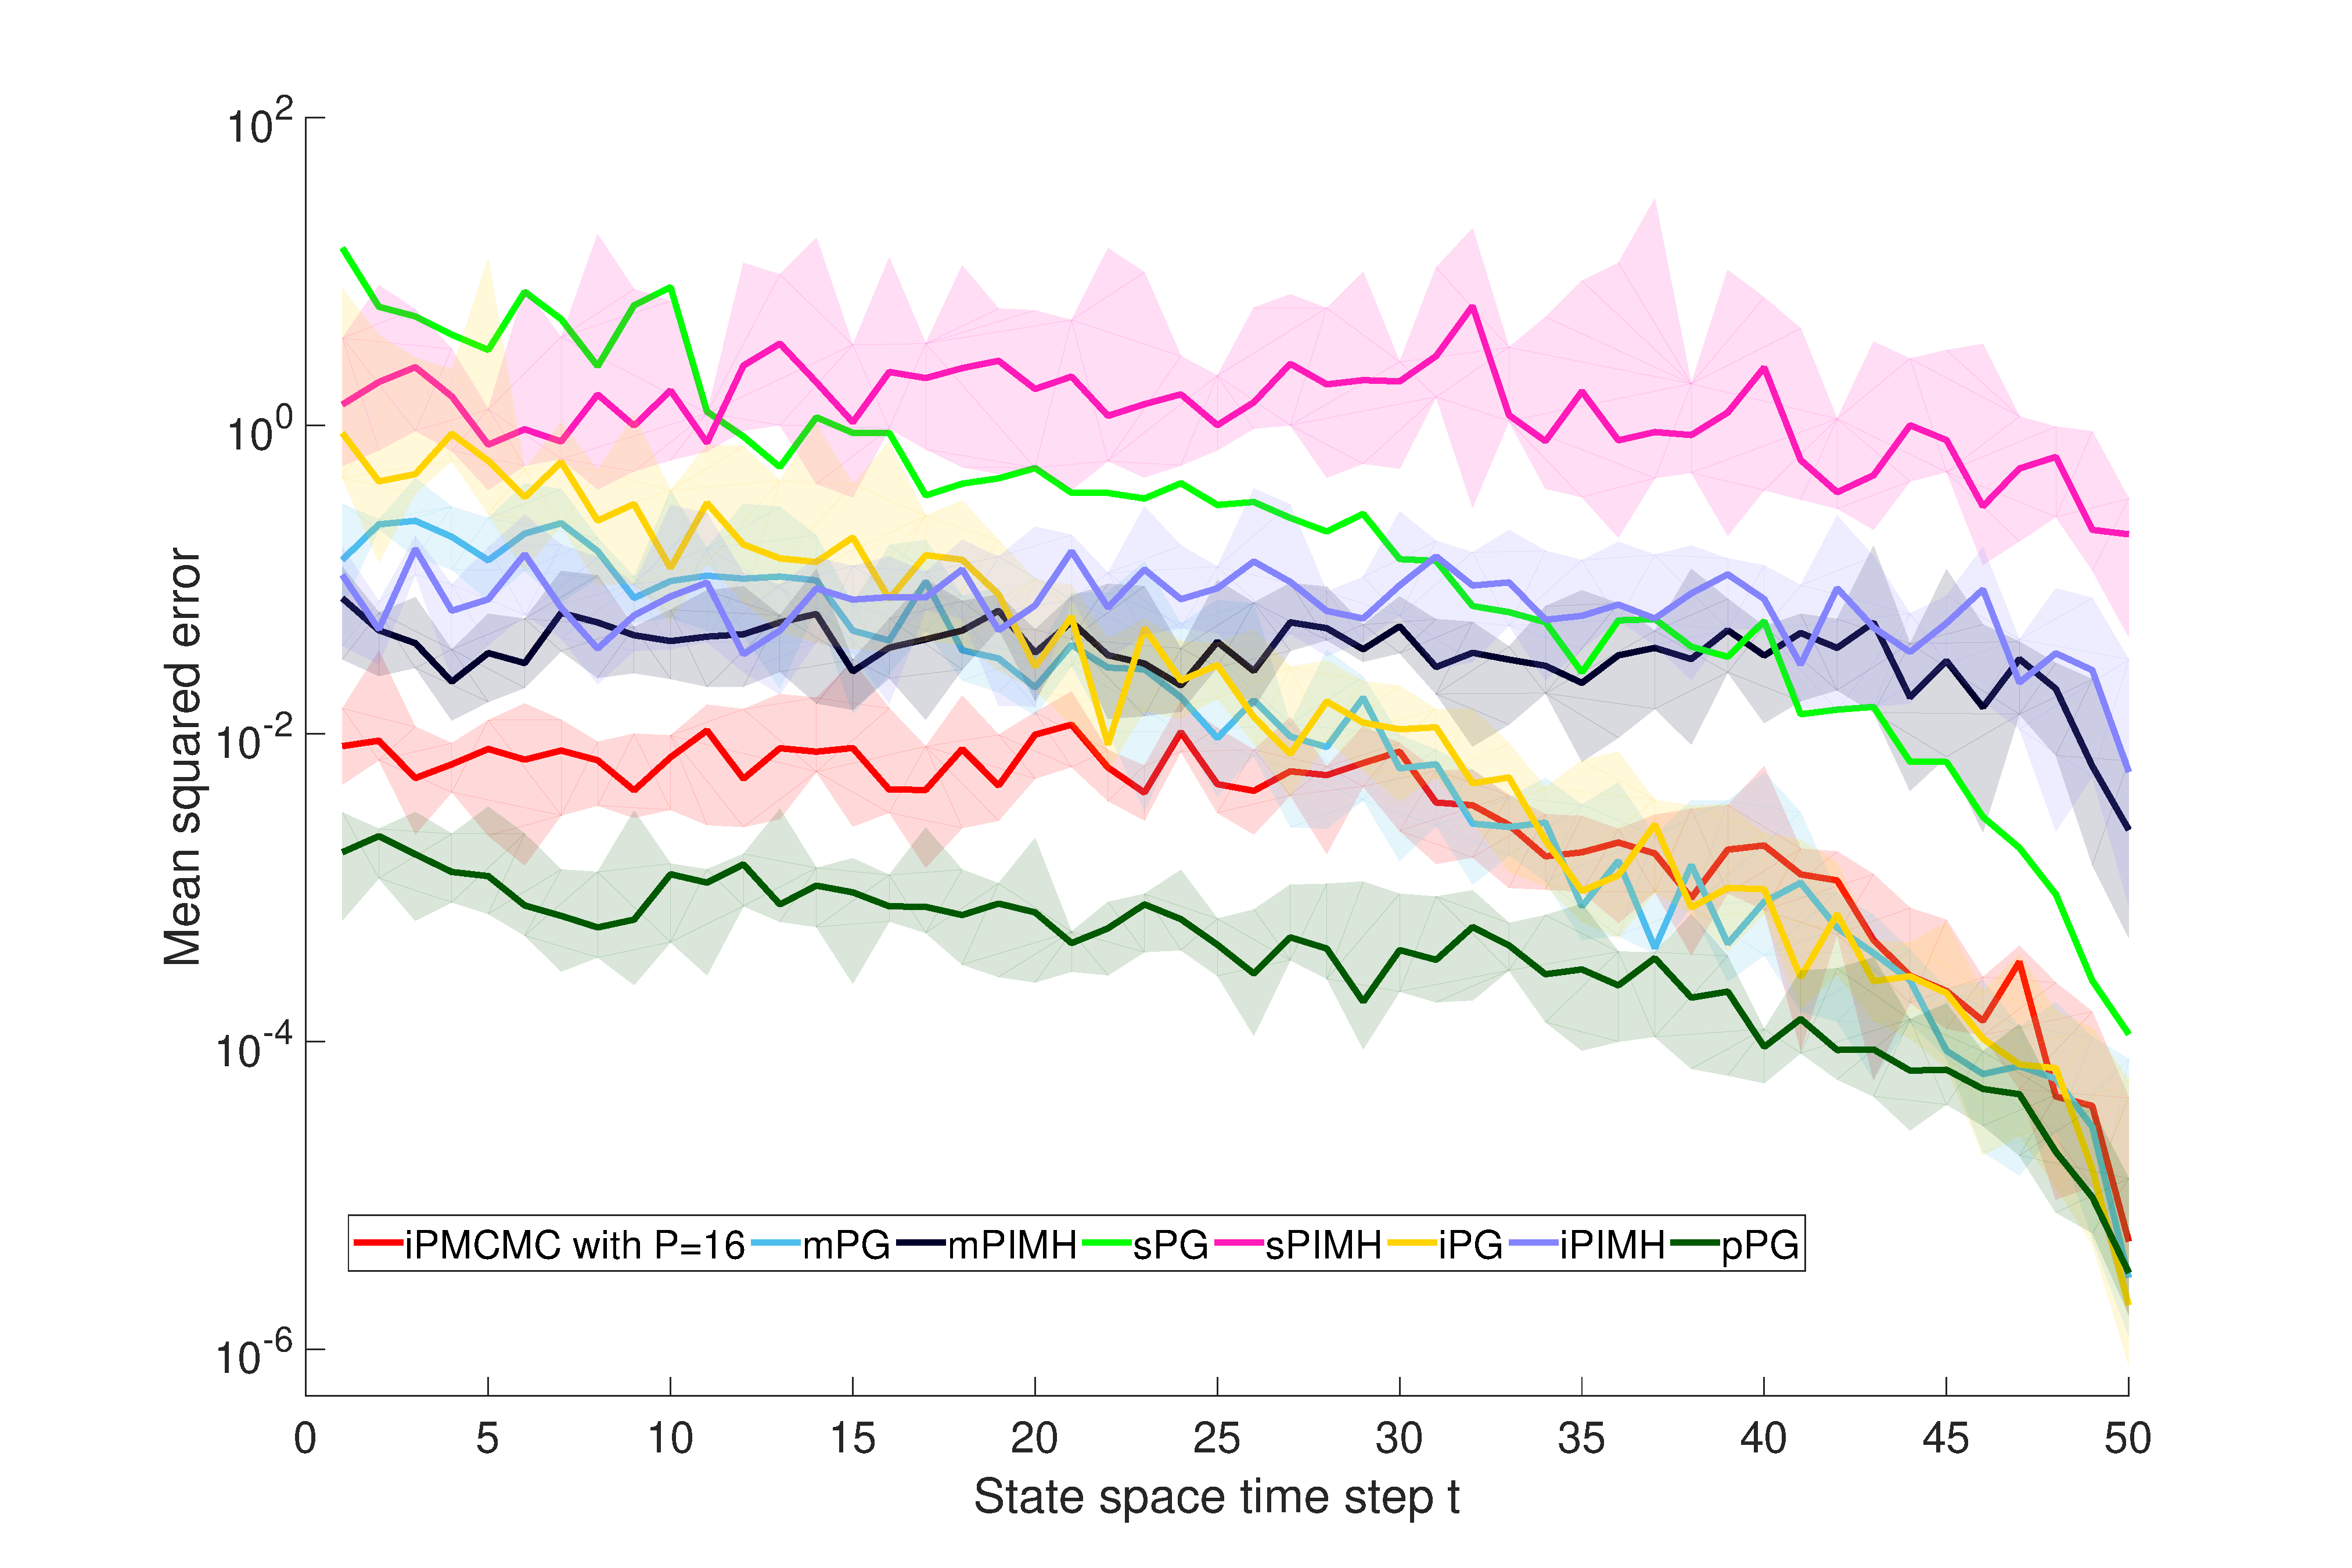
\includegraphics[width=1.1\textwidth,trim={4cm 0 5cm 0},clip]{kurtosis_pos_series_lss}}
		\caption{Final error in kurtosis}
		\label{fig:supp-kurt_series_pos}
	\end{subfigure}	
	
	
	\caption{Mean squared error in latent variable skewness and kurtosis averaged of all dimensions of the LGSSM as a function of MCMC iteration (left) and position in the state sequence (right) for iPMCMC, mPG, mPIMH and a number of serialized variants.  Key for legends: sPG = single PG chain, sPIMH = single PIMH chain, iPG = single PG chain run 32 times longer, iPIMH = single PIMH chain run 32 times longer and pPG = single PG with 32 times more particles.  For visualization purposes, the chains with extra iterations have had the number of MCMC iterations normalized by 32 so that the different methods represent equivalent total computational budget. \label{fig:supp-series_error_lss2}}
\end{figure*}

\begin{figure*}[p]
	\centering
	\begin{subfigure}[t]{0.49\textwidth}
		\makebox[\textwidth][r]{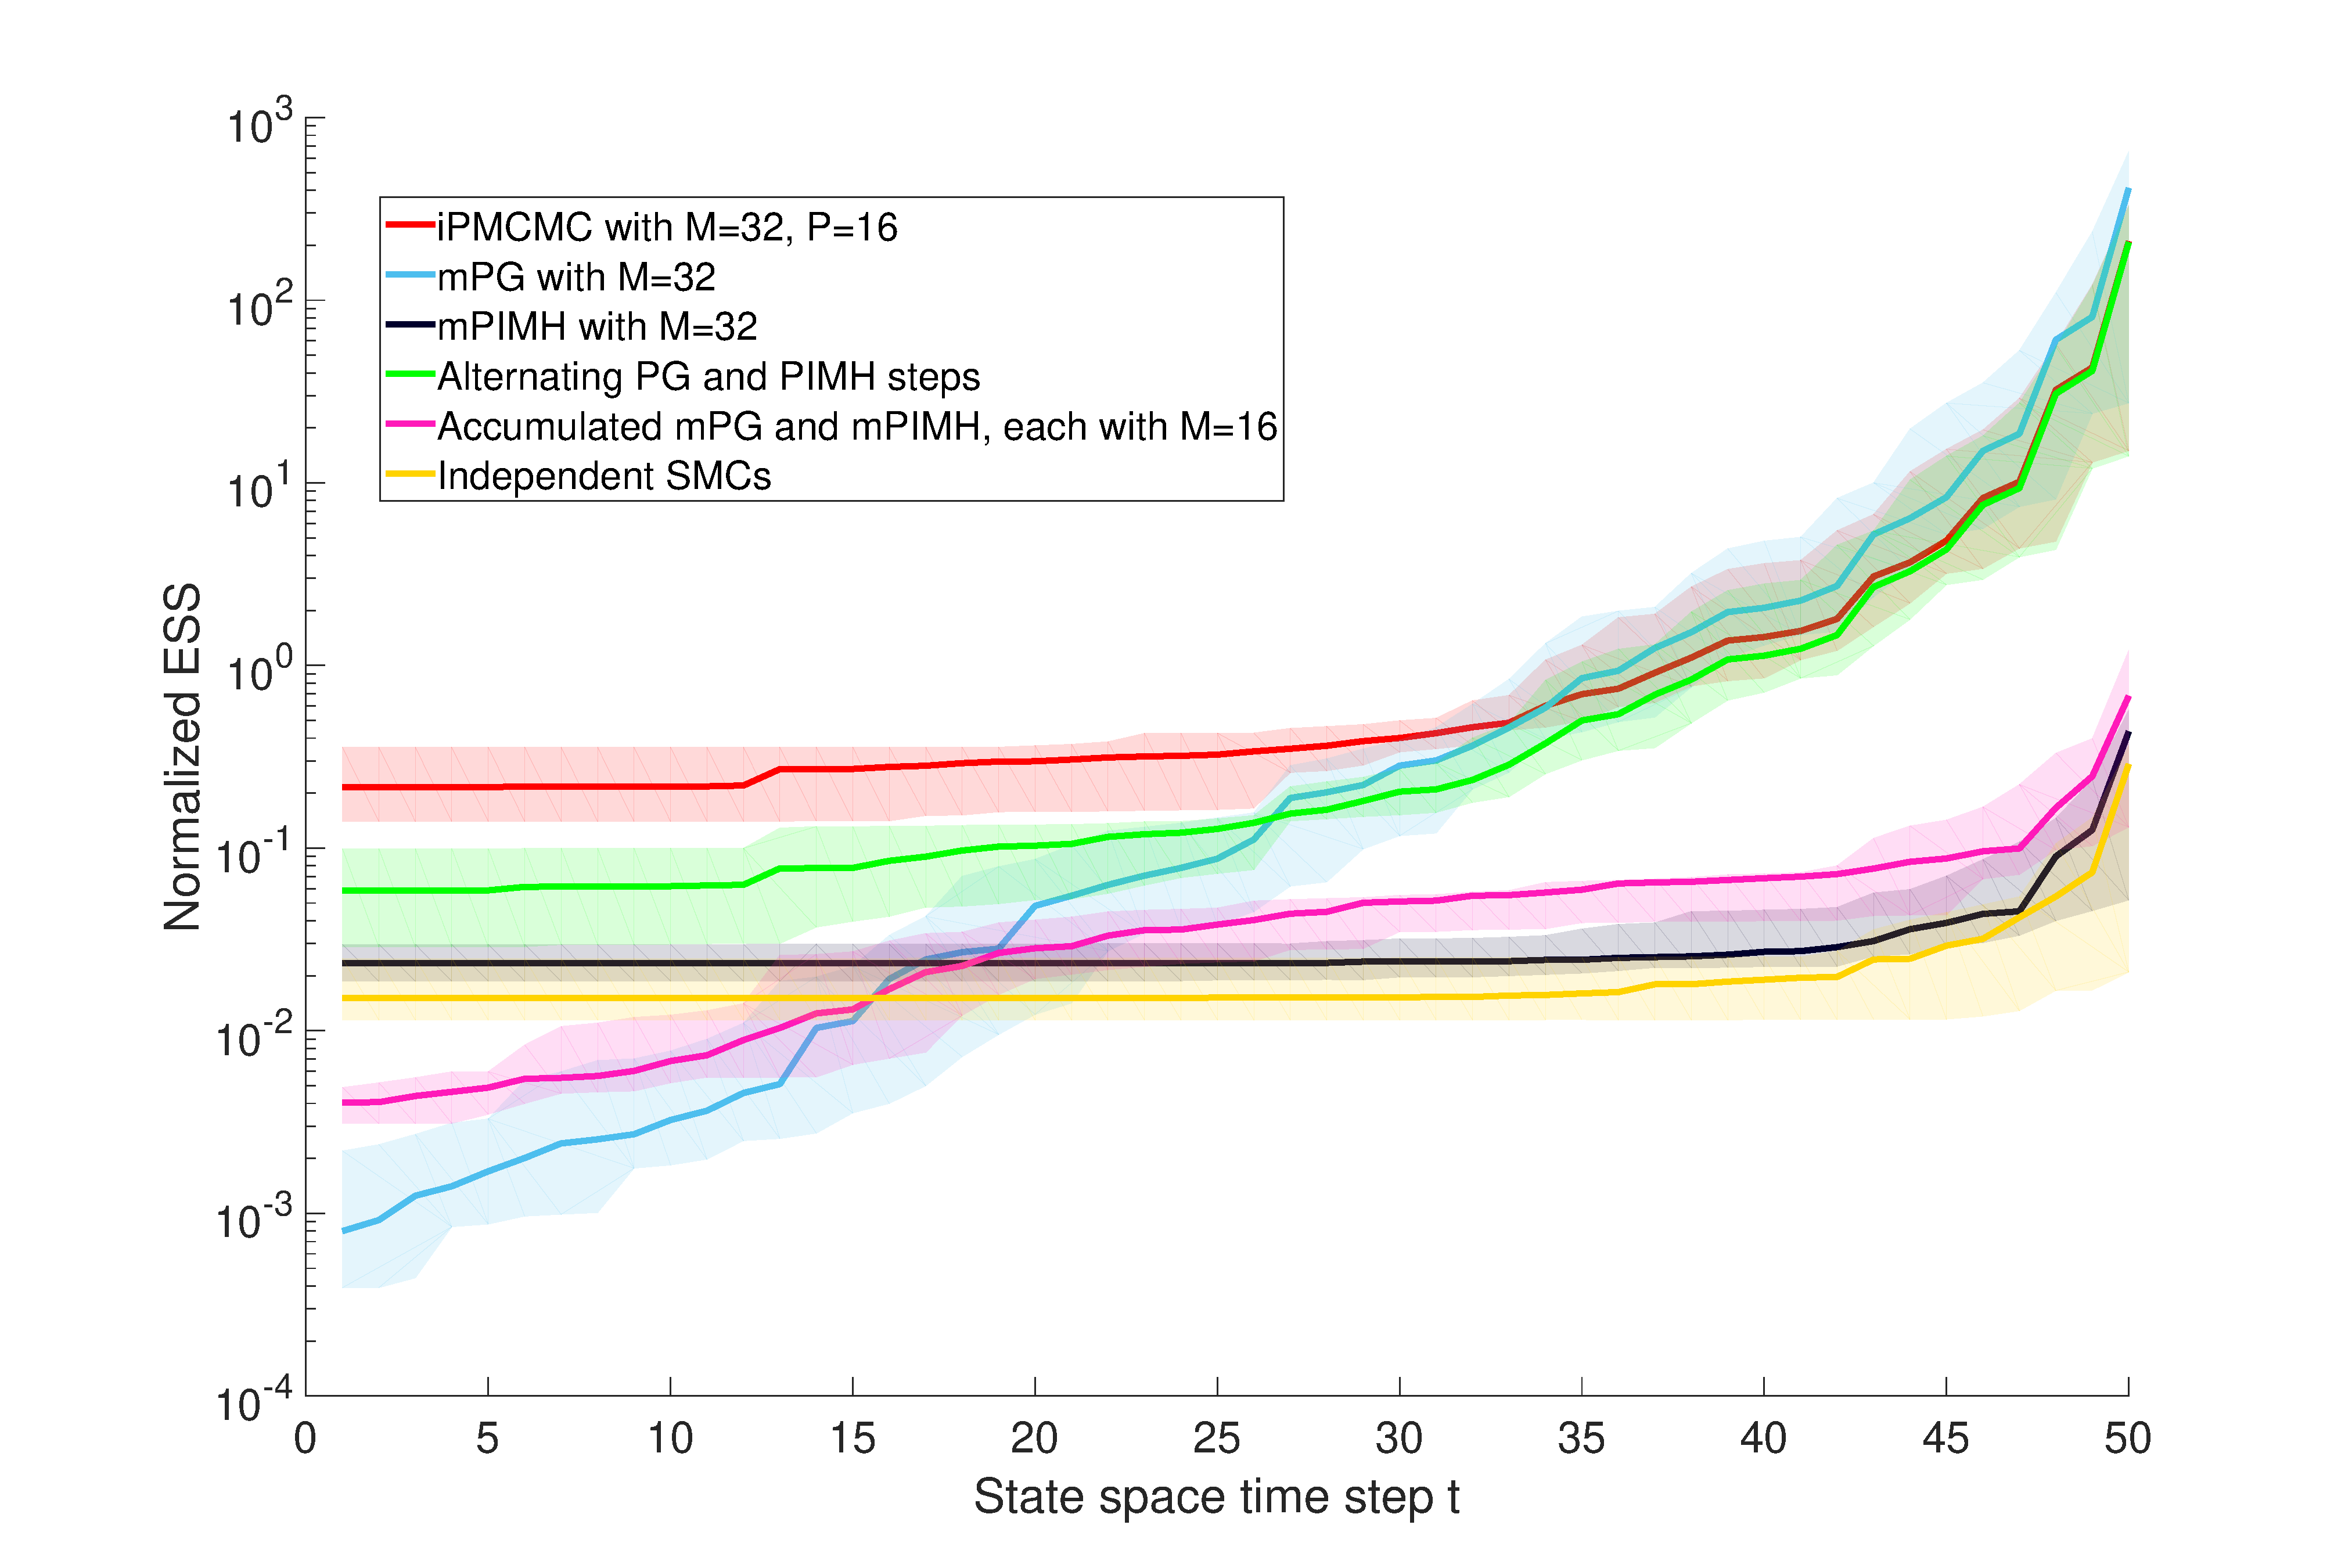
\includegraphics[width=1.1\textwidth,trim={4cm 0 5cm 0},clip]{ess_distributed_lss}}
		\caption{ESS of distributed methods for LGSSM}
		\label{fig:supp-ESS-lss-dist}
	\end{subfigure}
	~ %add desired spacing between images, e. g. ~, \quad, \qquad, \hfill etc. 
	%(or a blank line to force the subfigure onto a new line)
	\begin{subfigure}[t]{0.49\textwidth}
		\makebox[\textwidth][l]{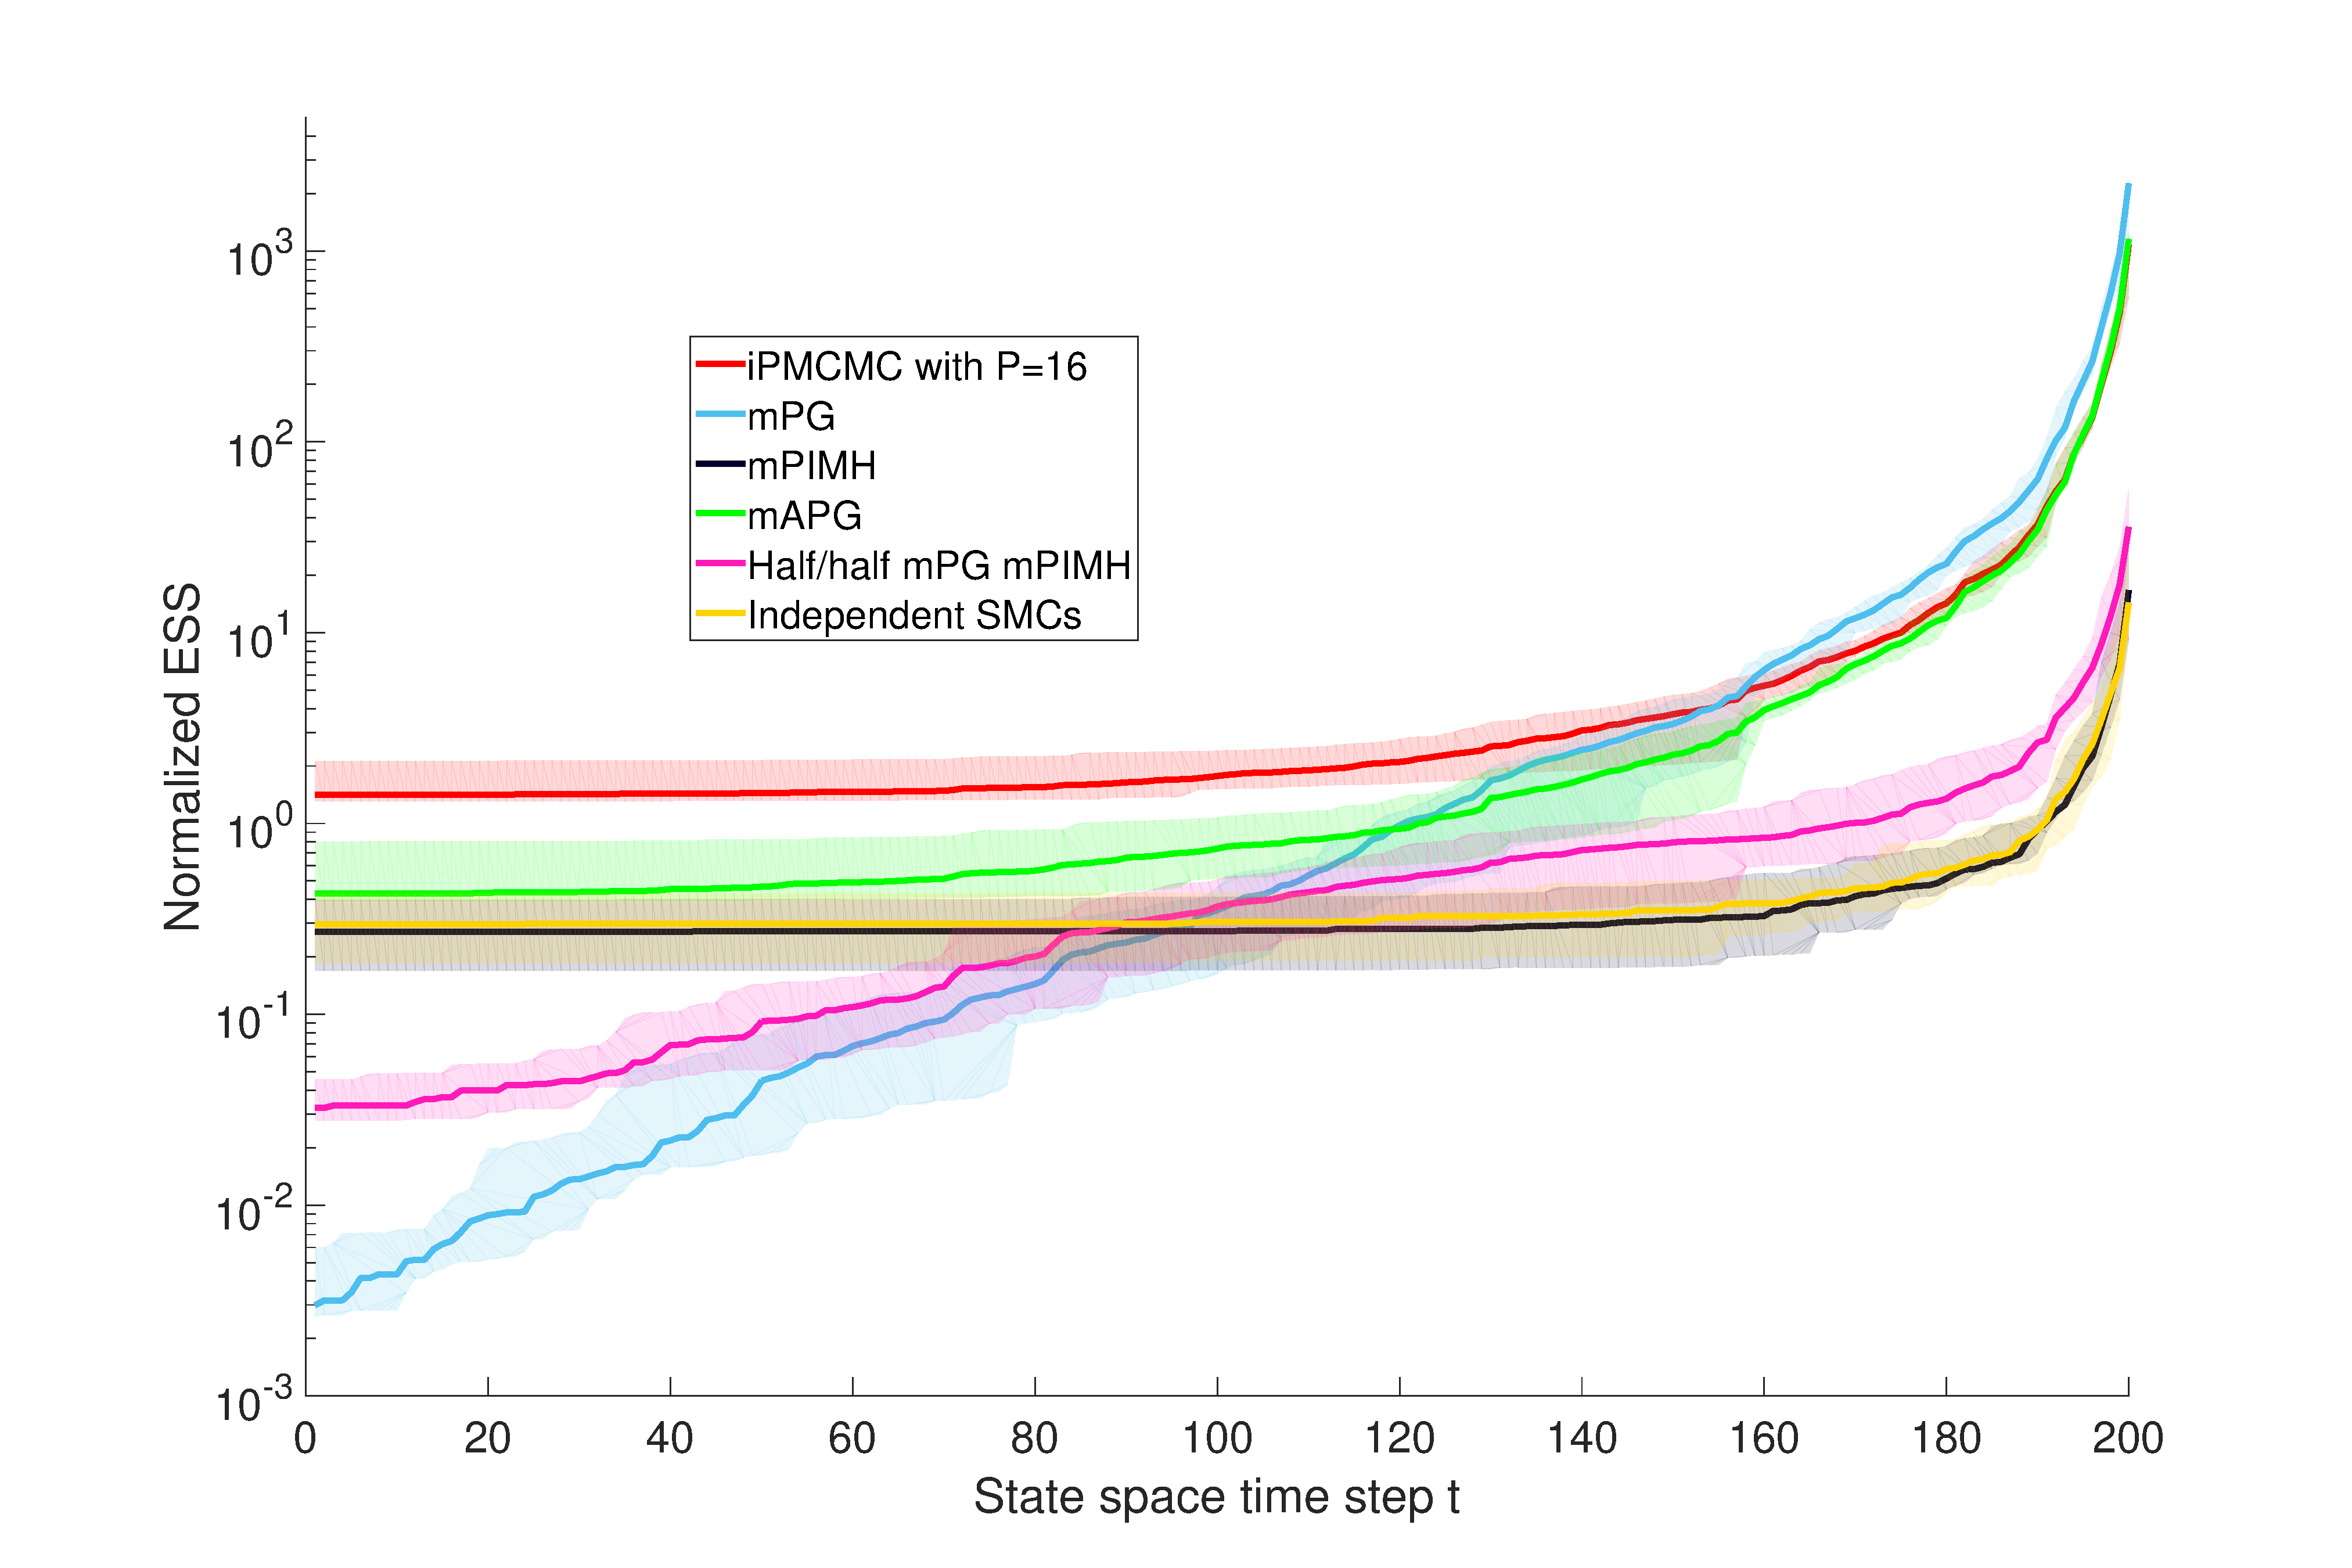
\includegraphics[width=1.1\textwidth,trim={4cm 0 5cm 0},clip]{ess_distributed_nlss}}
		\caption{ESS of distributed methods for NLSSM}
		\label{fig:supp-ESS-nlss-dist}
	\end{subfigure}
	
	\begin{subfigure}[t]{0.49\textwidth}
		\makebox[\textwidth][r]{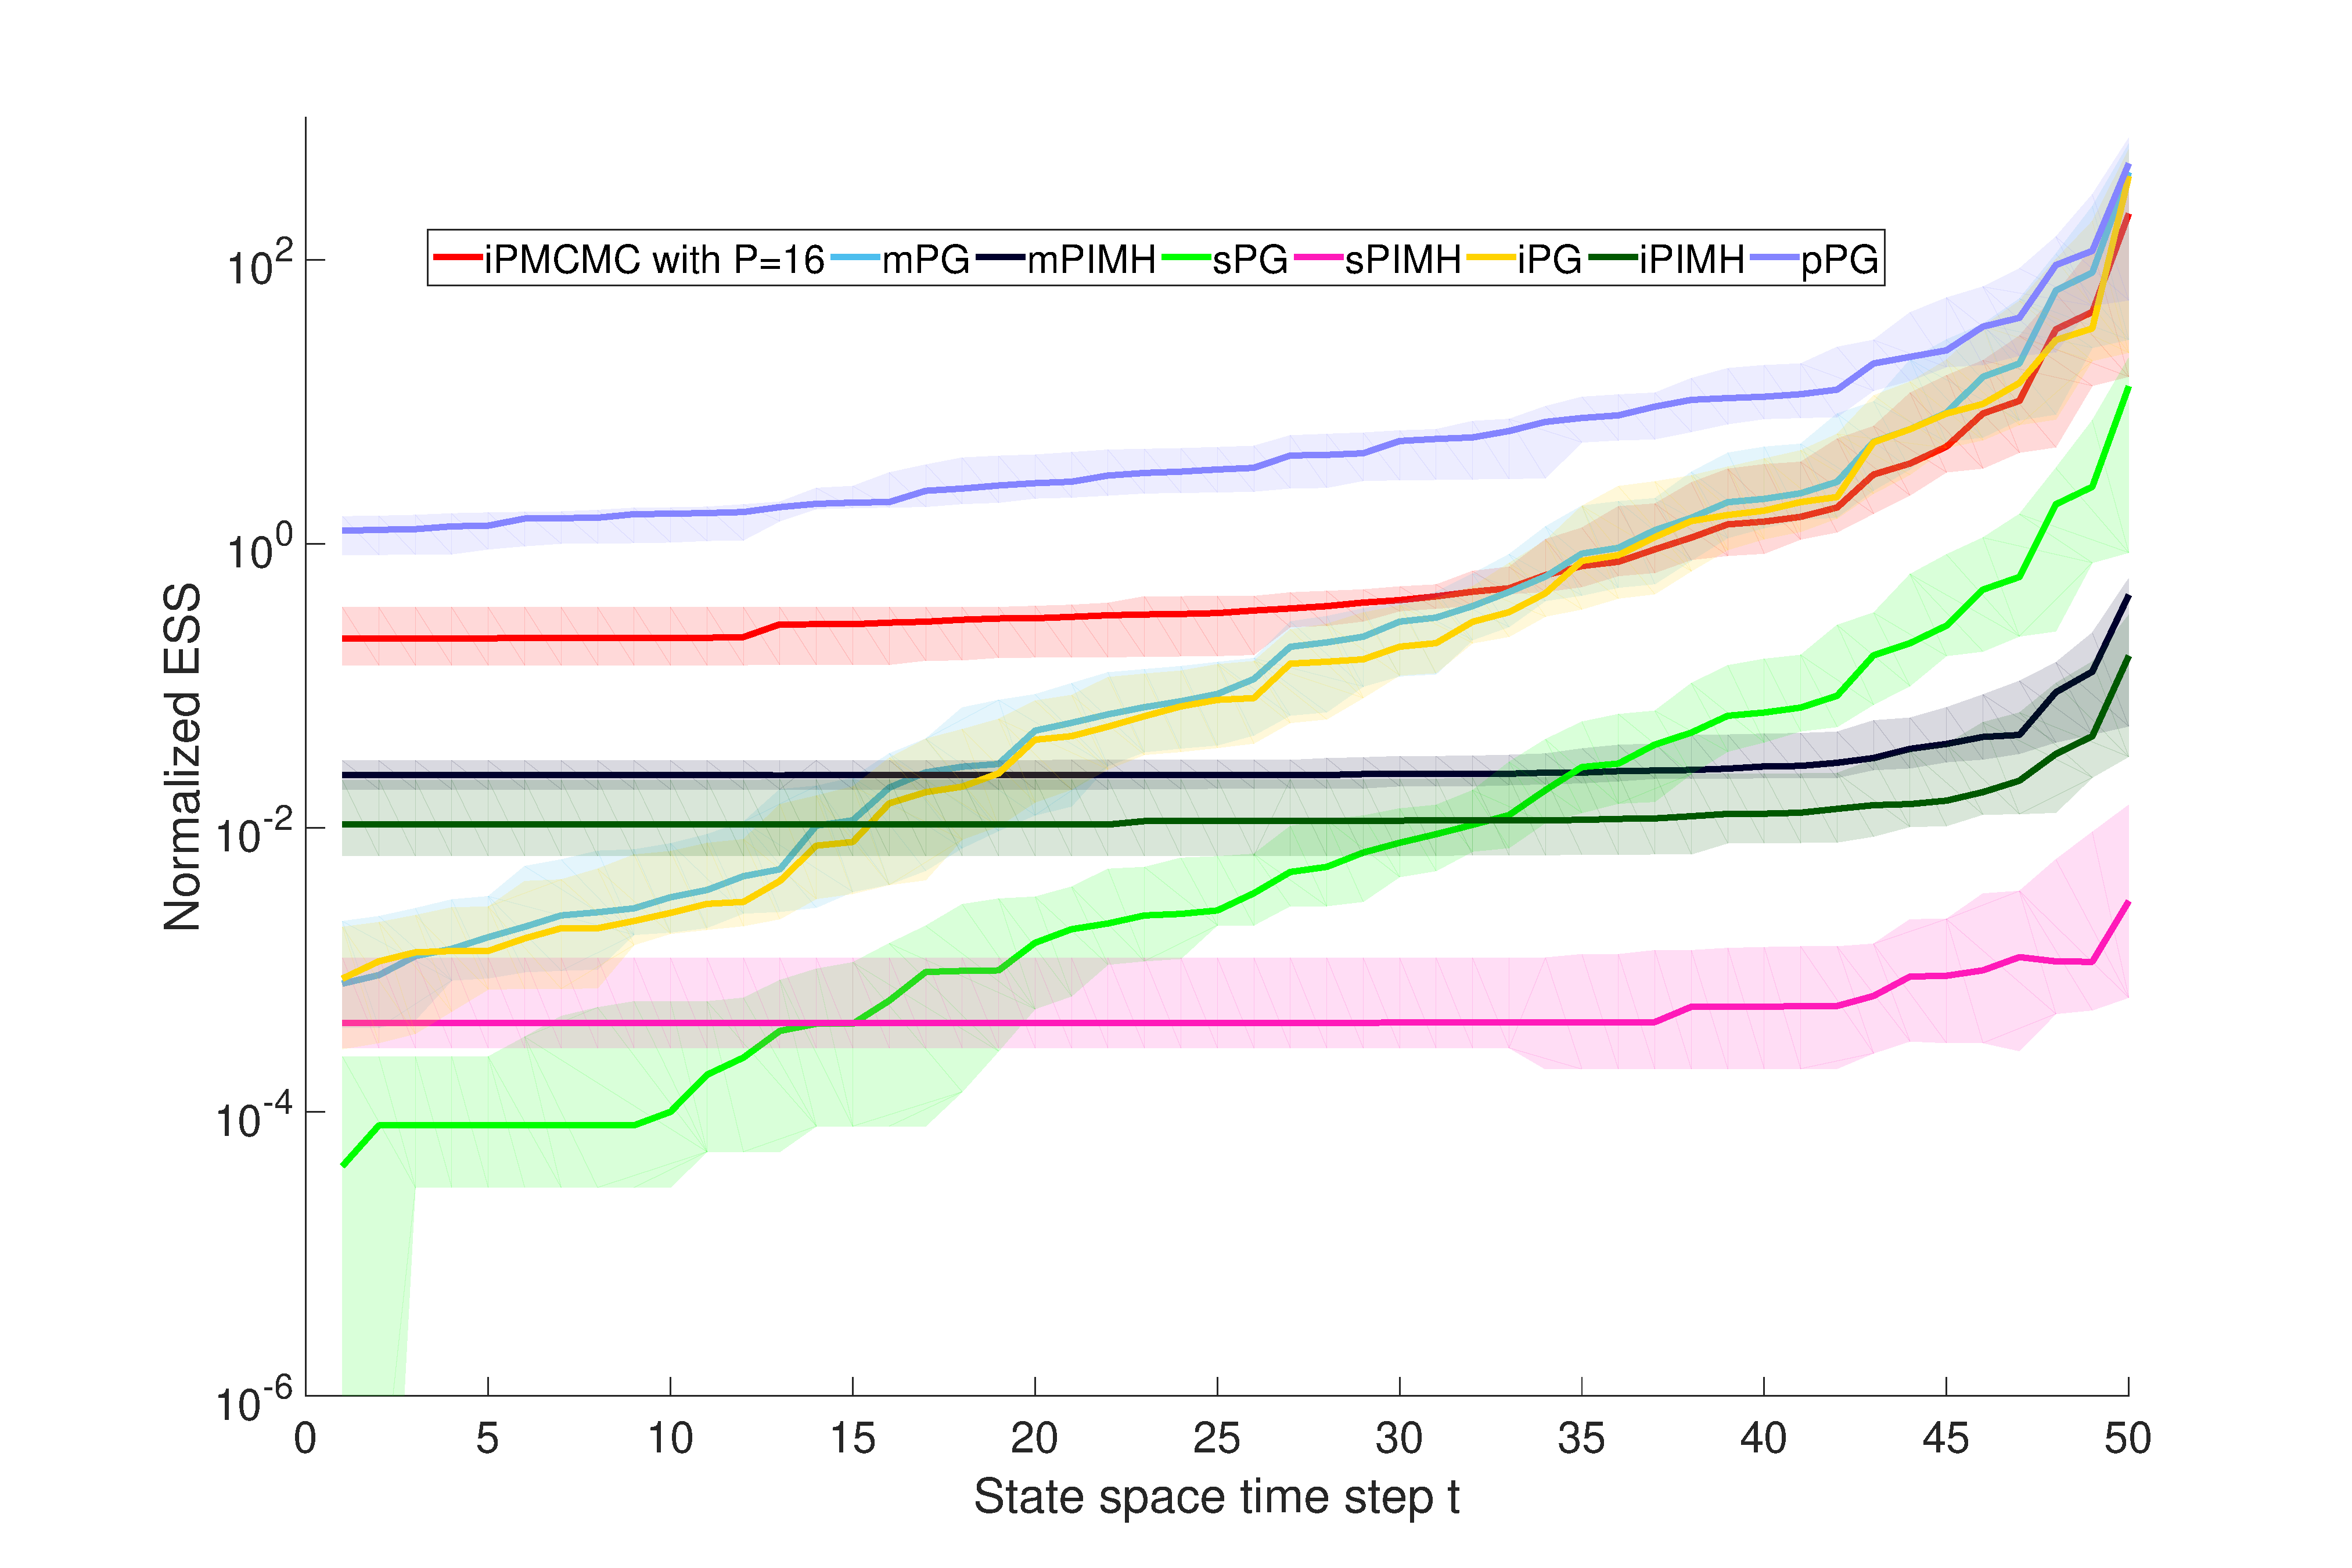
\includegraphics[width=1.1\textwidth,trim={4cm 0 5cm 0},clip]{ess_series_lss}}
		\caption{ESS comparison to series equivalents for LGSSM}
		\label{fig:supp-ESS-lss-series}
	\end{subfigure}
	~ %add desired spacing between images, e. g. ~, \quad, \qquad, \hfill etc. 
	%(or a blank line to force the subfigure onto a new line)
	\begin{subfigure}[t]{0.49\textwidth}
		\makebox[\textwidth][l]{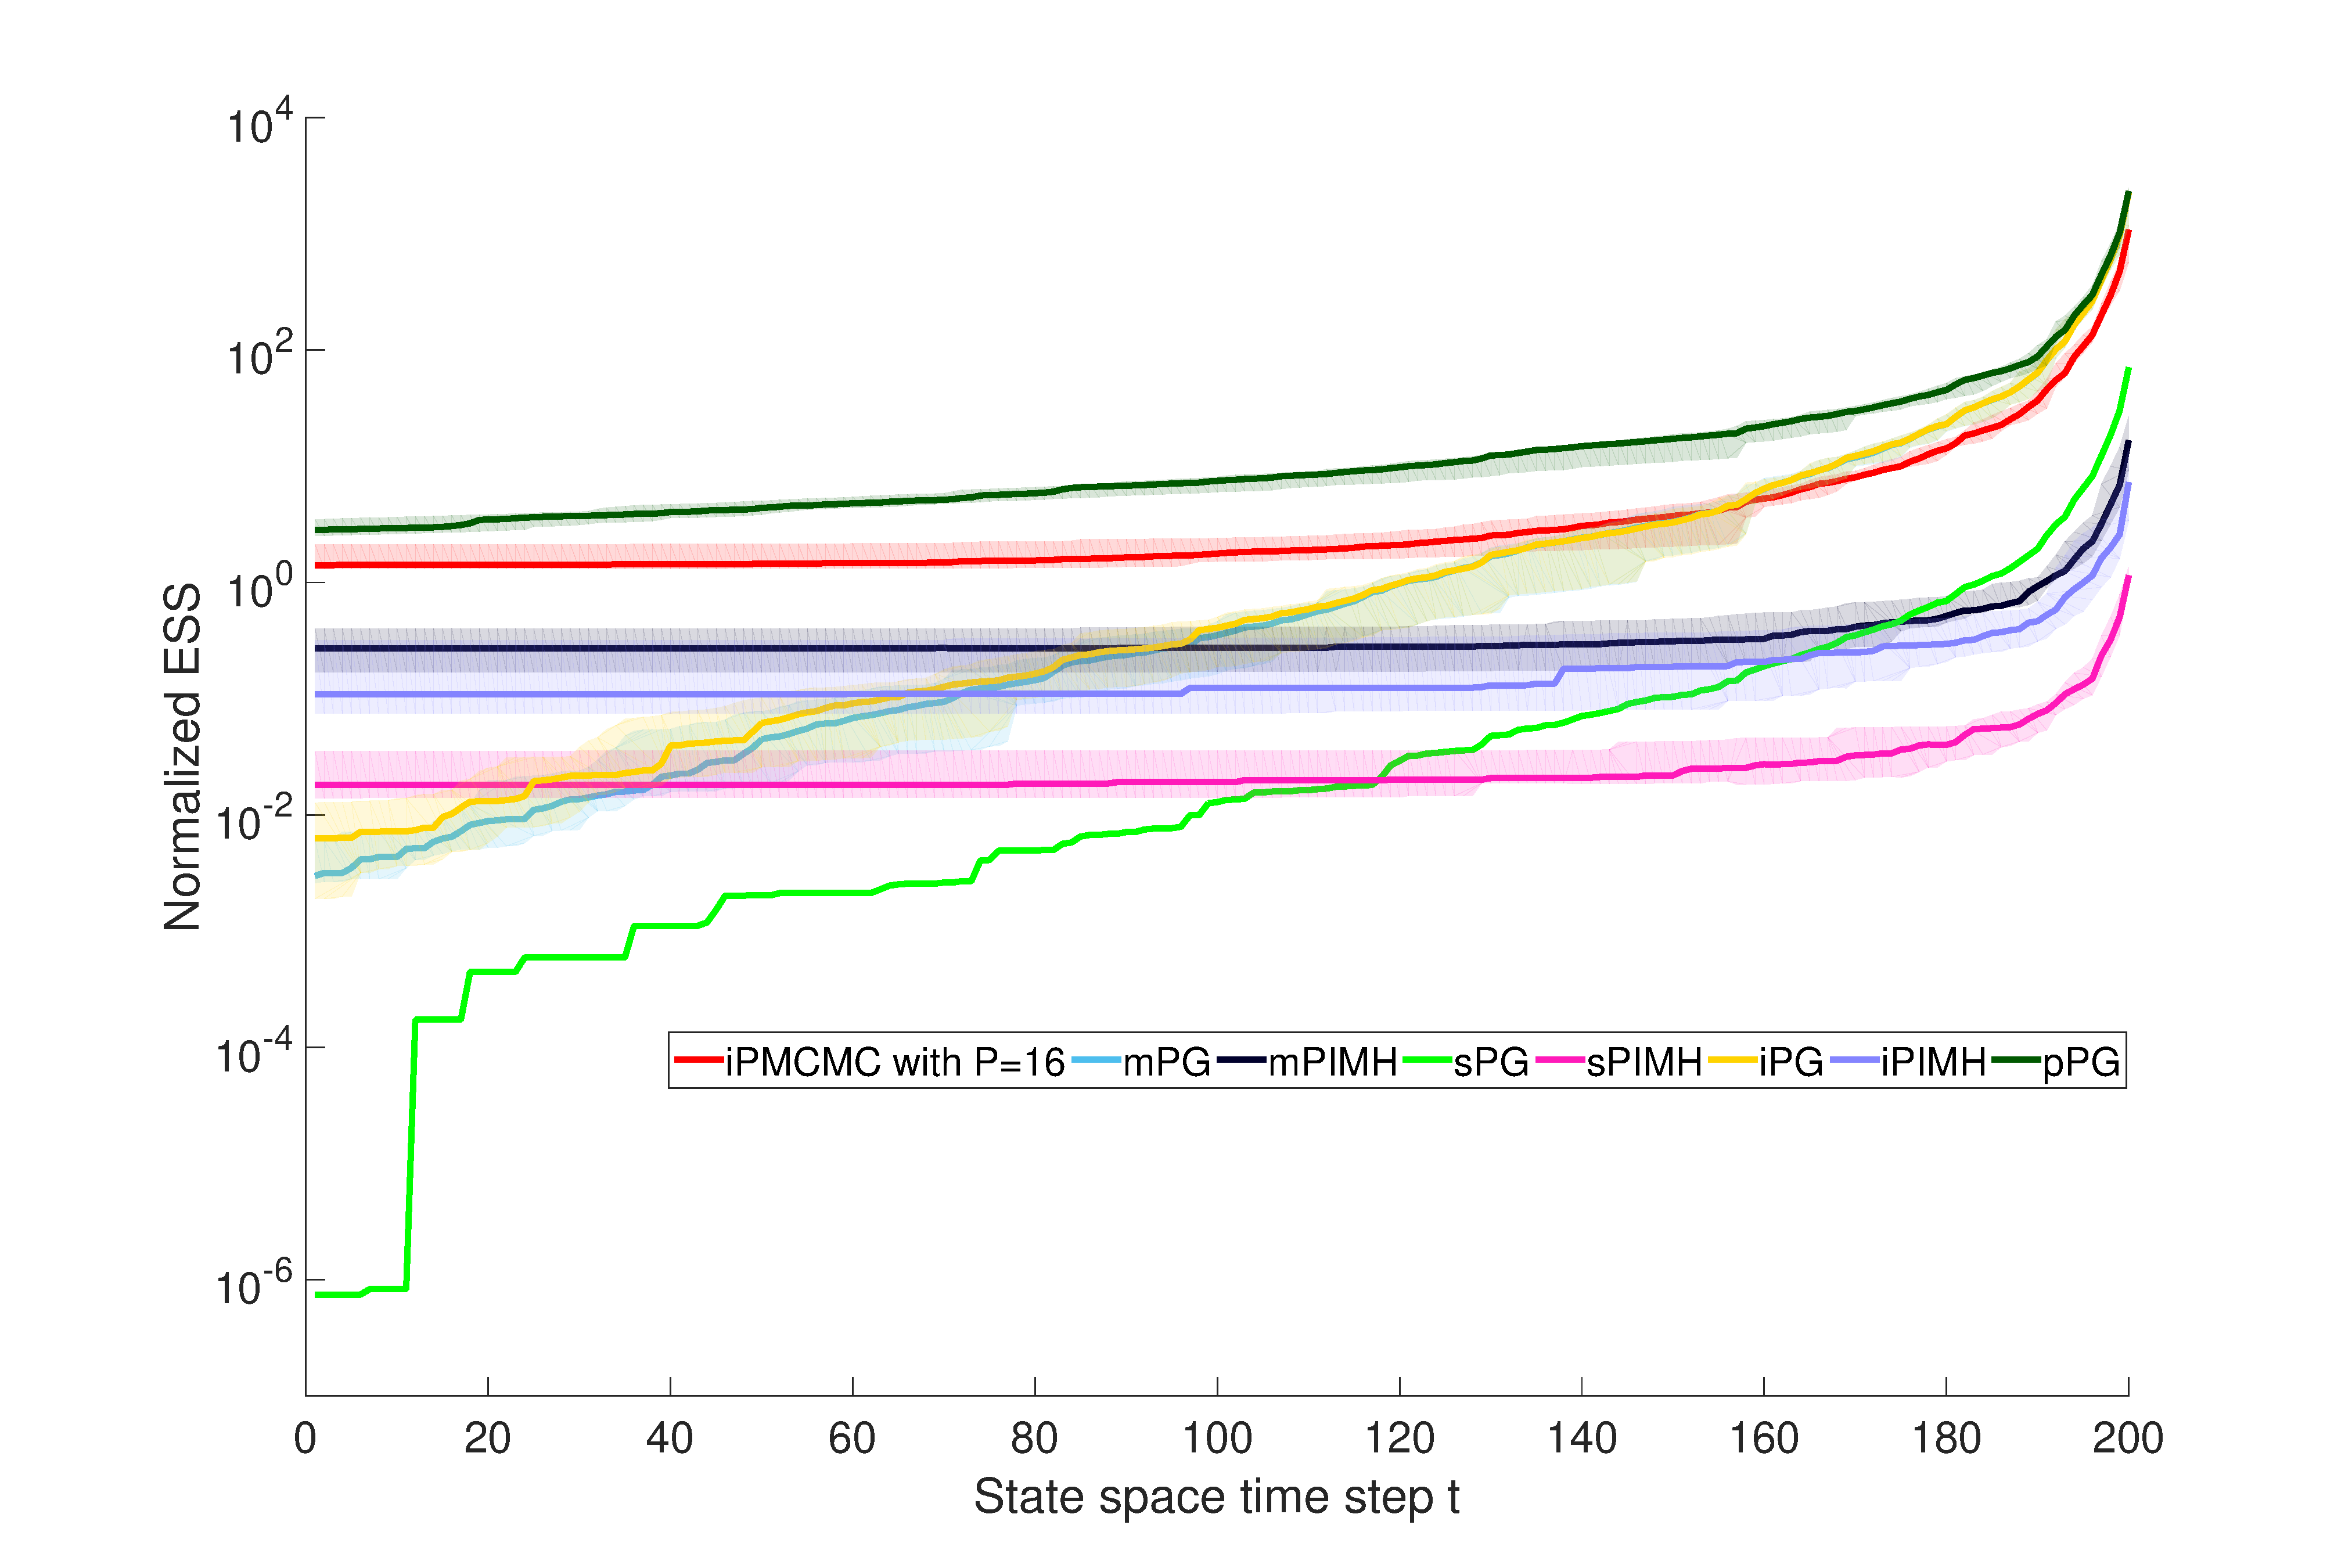
\includegraphics[width=1.1\textwidth,trim={4cm 0 5cm 0},clip]{ess_series_nlss}}
		\caption{ESS comparison to series equivalents for NLSSM}
		\label{fig:supp-ESS-nlss-series}
	\end{subfigure}	
	
	\caption{Normalized effective sample size for LGSSM (left) and NLSSM (right) for a number of distributed and series models.  Key for legends: sPG = single PG chain, sPIMH = single PIMH chain, iPG = single PG chain run 32 times longer, iPIMH = single PIMH chain run 32 times longer and pPG = single PG with 32 times more particles. \label{fig:supp-ess_extras}}
\end{figure*}
